% This file: 			Draft Compiling New Information and Analysis
% Contributors: 		Pietro Biroli, Daniela Del Boca, Linor Kiknadze,
%					Yu Kyung Koh, Sylvi Kuperman, Sidharth Moktan,
%					Chiara Pronzato, Anna Ziff
% Original date: 		10/3/16
% Project: 			Reggio Evaluation

%Style
\documentclass[12pt]{article}
\usepackage[top=1in, bottom=1in, left=1in, right=1in]{geometry}
\parindent 22pt
\usepackage{fancyhdr}

%Packages
\usepackage{adjustbox}
\usepackage{amsmath}
\usepackage{amsfonts}
\usepackage{amssymb}
\usepackage{bm}
\usepackage[table]{xcolor}
\usepackage{tabu}
\usepackage{makecell}
\usepackage{longtable}
\usepackage{multirow}
\usepackage[normalem]{ulem}
\usepackage{etoolbox}
\usepackage{graphicx}
\usepackage{tabularx}
\usepackage{ragged2e}
\usepackage{booktabs}
\usepackage{caption}
\usepackage{fixltx2e}
\usepackage[para, flushleft]{threeparttablex}
\usepackage[capposition=top]{floatrow}
\usepackage{subcaption}
\usepackage{pdfpages}
\usepackage{pdflscape}
\usepackage{natbib}
\usepackage{bibunits}
\definecolor{maroon}{HTML}{990012}
\usepackage[colorlinks=true,linkcolor=maroon,citecolor=maroon,urlcolor=maroon,anchorcolor=maroon]{hyperref}
\usepackage{marvosym}
\usepackage{makeidx}
\usepackage{tikz}
\usetikzlibrary{shapes}
\usepackage{setspace}
\usepackage{enumerate}
\usepackage{rotating}
\usepackage{epstopdf}
\usepackage[titletoc]{appendix}
\usepackage{framed}
\usepackage{comment}
\usepackage{xr}
\usepackage{titlesec}
\usepackage{footnote}
\usepackage{longtable}
\newlength{\tablewidth}
\setlength{\tablewidth}{9.3in}
\setcounter{secnumdepth}{4}

\titleformat{\paragraph}
{\normalfont\normalsize\bfseries}{\theparagraph}{1em}{}
\titlespacing*{\paragraph}
{0pt}{3.25ex plus 1ex minus .2ex}{1.5ex plus .2ex}
\makeatletter
\pretocmd\start@align
{%
  \let\everycr\CT@everycr
  \CT@start
}{}{}
\apptocmd{\endalign}{\CT@end}{}{}
\makeatother
%Watermark
\usepackage[printwatermark]{xwatermark}
\usepackage{lipsum}
\definecolor{lightgray}{RGB}{220,220,220}
%\newwatermark[allpages,color=lightgray,angle=45,scale=3,xpos=0,ypos=0]{Preliminary Draft}

%Further subsection level
\usepackage{titlesec}
\setcounter{secnumdepth}{4}
\titleformat{\paragraph}
{\normalfont\normalsize\bfseries}{\theparagraph}{1em}{}
\titlespacing*{\paragraph}
{0pt}{3.25ex plus 1ex minus .2ex}{1.5ex plus .2ex}

\setcounter{secnumdepth}{5}
\titleformat{\subparagraph}
{\normalfont\normalsize\bfseries}{\thesubparagraph}{1em}{}
\titlespacing*{\subparagraph}
{0pt}{3.25ex plus 1ex minus .2ex}{1.5ex plus .2ex}

%Functions
\DeclareMathOperator{\cov}{Cov}
\DeclareMathOperator{\var}{Var}
\DeclareMathOperator{\plim}{plim}
\DeclareMathOperator*{\argmin}{arg\,min}
\DeclareMathOperator*{\argmax}{arg\,max}

%Math Environments
\newtheorem{theorem}{Theorem}[section]
\newtheorem{claim}[theorem]{Claim}
\newtheorem{assumption}[theorem]{Assumption}
\newtheorem{definition}[theorem]{Definition}
\newtheorem{hypothesis}[theorem]{Hypothesis}
\newtheorem{property}[theorem]{Property}
\newtheorem{example}[theorem]{Example}
\newtheorem{condition}[theorem]{Condition}
\newtheorem{result}[theorem]{Result}
\newenvironment{proof}{\paragraph{Proof:}}{\hfill$\square$}

%Commands
\newcommand\independent{\protect\mathpalette{\protect\independenT}{\perp}}
\def\independenT#1#2{\mathrel{\rlap{$#1#2$}\mkern2mu{#1#2}}}
\newcommand{\overbar}[1]{\mkern 1.5mu\overline{\mkern-1.5mu#1\mkern-1.5mu}\mkern 1.5mu}
\newcommand{\equald}{\ensuremath{\overset{d}{=}}}
\captionsetup[table]{skip=10pt}
%\makeindex


\newcolumntype{L}[1]{>{\raggedright\let\newline\\\arraybackslash\hspace{0pt}}m{#1}}
\newcolumntype{C}[1]{>{\centering\let\newline\\\arraybackslash\hspace{0pt}}m{#1}}
\newcolumntype{R}[1]{>{\raggedleft\let\newline\\\arraybackslash\hspace{0pt}}m{#1}}



%Logo
%\AddToShipoutPictureBG{%
%  \AtPageUpperLeft{\raisebox{-\height}{\includegraphics[width=1.5cm]{uchicago.png}}}
%}

\newcolumntype{L}[1]{>{\raggedright\let\newline\\\arraybackslash\hspace{0pt}}m{#1}}
\newcolumntype{C}[1]{>{\centering\let\newline\\\arraybackslash\hspace{0pt}}m{#1}}
\newcolumntype{R}[1]{>{\raggedleft\let\newline\\\arraybackslash\hspace{0pt}}m{#1}} 

\newcommand{\mr}{\multirow}
\newcommand{\mc}{\multicolumn}

%\newcommand{\comment}[1]{}


\externaldocument{reggioEvaluation_appendix}

\begin{document}

\title{\Large \textbf{Evaluation of the Reggio Approach} \\ Draft}
\author{\normalsize Reggio Team}
\date{\normalsize Original version: October 3, 2016 \\ Current version: \today}
\maketitle

\textbf{[JJH: Many questions -- we are not apologists for Reggio. The \emph{ad hoc} adjustment to matching bothers me. I do not see a good justification and $\Pi$ is estimated. Let's finish. We need to: (1) Put the infant toddler outcomes in main text. We have results. The fact that they are not present in other cities is a huge advantage. (2) Report step down for each column and each table. (3) Identify in each table the group being studied. (4) In the text, we need to summarize main finding of appendix in the text.]}

\tableofcontents

\clearpage
\doublespacing

\section{Introduction}
\label{sec:introduction}
The Reggio Approach is a birth to age-6 early childhood program implemented in Reggio Emilia, Italy starting in the early 1960s. It is based on a vision of the child as an individual with rights and potential. It has been a source of inspiration for hundreds of early childhood centers around the world.\footnote{The official \href{http://www.reggiochildren.it/network/?lang=en}{Reggio Children International Network} is present in 33 countries worldwide.} Reggio Approach schools have been awarded numerous prizes.\footnote{Examples include the Danish LEGO Prize (1992), the Kohl Foundation of Chicago award (1993), the Hans Christian Anderson Prize (1994), the Mediterranean Association of International Schools award (1994), the award from the French city of Blois (2001).} Despite its widespread recognition, the Reggio Approach has never been formally evaluated and there is no rigorous empirical evidence of its effects on children's life-cycle outcomes.

This paper presents an evaluation of the Reggio Approach using non-experimental comparison groups constructed from data on individuals from five different age cohorts (three cohorts of adults, one cohort of adolescents, and one cohort of children in their first year of elementary school) in three different cities: Reggio Emilia, Parma, and Padova. Although Parma and Padova are geographically close to Reggio Emilia and similar in economic and demographic characteristics, they have somewhat different preschool systems as described below. The individuals in each city are exposed to one of four different early childhood experiences: municipal, state, religious, or none. The Reggio Approach is delivered through the municipal early childhood schools of Reggio Emilia. Our evaluation strategy consists of comparing the outcomes of those who attended municipal institutions in Reggio Emilia (treatment group) to those who experienced other preschool types (including no preschool) either in Reggio Emilia or in Parma and Padova (control groups).

Our evaluation of the Reggio Approach faces several challenges. First, the non-experimental nature of the data raises concerns about bias from self-selection of individuals into different early childhood programs. We employ a number of econometric techniques in an attempt to control for potential selection problems. Second, there is a prevalence of other high-quality childcare programs in Northern Italy that enroll many youth. In the mid-20th century, Northern Italy witnessed a rise in local early childhood programs many of which were influenced by Loris Malaguzzi as well as other respected early childhood experts \citep{OECD_2001_Italy-Country-Note}. This rise in quality of childcare alternatives was accompanied by an increase in the preschool attendance rate of Italian children aged 3-6 years from 50\% in the 1960s to 96\% in the 1990s \citep{Hohnerlein_2015_Development-and-Diffusion}. The common influences across regions in our control group pose serious problems for any analysis based on comparison groups across cities in the region.  The evidence of common preschool practices currently in place in northern Italy is consistent with two interpretations: (i) that a common influence was at work across towns; or (ii) that the Reggio program was unique, but its essential elements diffused rapidly across towns and alternative schools within the same towns. Malaguzzi was active in promoting high-quality preschool throughout northern Italy.

In this paper, we compare individuals who attended Reggio Approach programs with those who attended other center-based programs within Reggio and in our comparison cities. These estimates capture the benefits of attending the Reggio Approach programs relative to other center-based programs. They are generally small and statistically insignificant. However, when we compare individuals who attended Reggio Approach schools with those who did not attend any center-based program, we find beneficial effects.

In contextualizing our findings, it is essential to understand the heterogeneity in early childhood approaches across school types, cities, and cohorts. Towards this end, Section~\ref{sec:ece-italy} presents key findings from an extensive review of the literature as well as results from a survey we conducted to quantify differences in administrative and pedagogical components among the different school types in the three cities. The survey allows us to track the evolution of differences in approaches in early childhood across cities and across school-types within cities. It is designed to elicit the availability of preschool and infant-toddler centers to cohorts of different ages in our sample. Results from our survey show that non-Reggio-Approach schools have historically shared many of the same characteristics with Reggio Approach schools, and that the commonalities of these characteristics increase over time (across cohorts). Given the overlap in these characteristics, it is reasonable to expect that comparisons of outcomes for Reggio Approach attendees with outcomes for those who attended alternative programs produce small, possibly negligible, treatment effects.

Results differ across age cohorts and with respect to the control group used. With the exception of some non-cognitive outcomes, we do not find any consistently statistically significant positive effects of the Reggio Approach on children and adolescents. Our most favorable comparisons are for the age-40 adult cohort when we compare Reggio Approach individuals with those from Reggio Emilia who did not attend preschool. Positive and statistically significant effects are estimated for employment, non-cognitive skills, and voting behavior. We do not reject the hypothesis that attending Reggio Approach preschools improved outcomes relative to not attending preschool.

However, when we compare outcomes for Reggio Approach attendees with those who attended alternative preschools within the city, few statistically significant effects are found. If any appear, they are found for the oldest cohorts. The lack of positive and statistically significant results remains when we make comparisons with those who attended municipal programs in other cities, especially Padova.\footnote{This is consistent with historical information about the lower availability of alternative preschools at this time and the unavailability of the municipal system in Padova before the age-30 cohorts.} We do not reject the hypothesis that attending Reggio Approach preschools did not improve outcomes relative to attending other regional preschools. We reach similar conclusions for infant-toddler centers, but the data are much more sparse.

The rest of the paper is organized in the following way. Section \ref{sec:ece-italy} describes the Reggio Approach. We discuss childcare programs in our three comparison group cities drawing from historical records and a survey we constructed and administered to officials across the different areas. Section \ref{sec:data} describes the research design, including the selection of cities, the survey data collection, and the questionnaires. Section \ref{sec:methodology} presents the methods used to estimate the Reggio treatment effects. Section \ref{sec:result} presents our estimates. Section \ref{sec:discussion} discusses the results in the context of historical information on different childcare programs.



\section{Early Childhood Programs in Northern Italy}
\label{sec:ece-italy}
Our study compares individuals who experienced the Reggio Approach with those who experienced other Northern Italian early childhood programs, as well as some who undertook no program at all. In this section, we document the Reggio Approach and explore the extent to which other early childhood programs in Reggio Emilia, Parma, and Padova implemented features of the Reggio Approach at different points of time.

\subsection{Municipal Early Childhood Schools of Reggio Emilia - The Reggio Approach}

Of the municipal systems in Reggio Emilia, Parma, and Padova, the Reggio Approach is notable for creative programming \textbf{[JJH: Innovative how? Please cut the bombast.][Edited to be more precise.]}, investment in staffing, early inclusion of children with disabilities, and high rates of provision of early childhood services. Of the three, Reggio Emilia was the first to develop a municipal early childhood system. It funds and manages the largest number of municipal infant-toddler and preschool sites.\footnote{Similar to Parma and Padova, Reggio Emilia contracts with local private providers and cooperatives to offer infant-toddler and preschool slots according to municipal regulations. These ``affiliated'' programs may not follow the Reggio Approach nor the municipal approaches in Parma and Padova. Accordingly, we consider this a separate sample during analysis.} 

In 1963, Reggio Emilia constructed its first municipal preschool for children aged 3-6 years; by 1975, the municipality offered 19 preschools \citep{Hohnerlein_2009_Paradox-Public-Preschools}. In 1965, the municipality legislated funding for infant-toddler centers for children aged 3 to 36 months. The first childcare site opened in 1971, and another 10 were added by 1979 \citep{Cagliari-etal-eds_2016_BOOK_Loris-Malaguzzi}. The municipal early childhood system in Reggio Emilia thus preceded Italy's key educational reforms of 1968 and 1971 which legislated free state preschools and local provision of infant-toddler childcare. \textbf{[JJH: Can we say that Reggio actually influenced reforms? Sylvi: I don't recommend saying this because Hohnerlein, a non-Reggio scholar, credits Bruno Ciari (and not Malaguzzi) for influencing the 1968 state reforms for public preschool. By citing the 2001 OECD report authored by FPGC scholar Rebecca New, however, we can state that Malaguzzi's influence came after the early 1970s, mainly in techniques to better engage families and in pedagogy (i.e., creativity as a vehicle for learning, use of pedagogistas, arts educators). The 2016 Malaguzzi book states that Reggio Emilia hosted 2 large conferences attended by 900 educators in the early 1970s to disseminate their new approaches throughout Italy. Shall we state this?]}

The Reggio Approach is a form of progressive early childhood education shaped by Loris Malaguzzi, a psychologist and educator influenced by Dewey's model of progressive education, Vygotsky, and the psychological theories of Piaget, Erikson, Bronfenbrenner, Bruner, and Gardner \citep{Rinaldi_2006_ReggioEmilia_BOOK,Cagliari-etal-eds_2016_BOOK_Loris-Malaguzzi} \textbf{[JJH: Do we know this? Please give me a citation. Talk is cheap and people rationalize what they did, see e.g., the Perry teacher survey. Did Reggio evolve? Gardner could not have had an effect. Sylvi: Regarding program evolution, according to the 2016 Malaguzzi book, the Reggio Approach features we reference in our survey were all in place by 1972. The book further cites the influence by the scholars listed above on Malaguzzi and the Reggio Approach. While Gardner came to Reggio after 1972, he provided teacher training and supported the use of creative arts in early childhood.]} Malaguzzi was also inspired by Bruno Ciari, who implemented Dewey's model in Bologna. Together, Ciari and Malaguzzi are credited with inciting a ``municipal school revolution'' in Italy by emphasizing learning, democratic participation, and social activism in early childhood, as an alternative to the welfare model and religious programming then-offered by the Catholic Church \citep{Lazzari_2012_Euro-J-Edu,Cagliari-etal-eds_2016_BOOK_Loris-Malaguzzi}.

In 1972, under Malaguzzi's direction, Reggio Emilia officially adopted Regulations for Municipal Schools that clarified the municipality's values for early childhood education, roles of parents and community members in municipal school management, staffing, professional development, enrollment priorities, and environmental features of preschools and infant-toddler centers \citep{Giaroni_1972_Regulations-Municipal-EC-Schools}. These regulations incorporate many of Ciari's innovations.\footnote{As director of municipal schools in Bologna from 1966-1970, Ciari promoted the physical learning environment, strong teacher-family relationships, participatory committees of parents and community members, and two co-teachers per classroom \citep{Edwards-etal-eds_1998_Hundred-Languages}.} 

From its inception, the engagement of families and the community was embedded in Reggio Approach practices. For example, parents and community members participate in school management to shape policies. Parents volunteer in classrooms and community members host field trips in the city \citep{CEHD_2016_Historical-Analysis,Cagliari-etal-eds_2016_BOOK_Loris-Malaguzzi}. To accommodate the needs of working parents, preschools and infant-toddler centers remain open five full-time days per week from September through June \citep{Giudici-Nicolosi_2014_Reggio-Approach}. Many municipal sites offer programming in July, and extended day options are available throughout the school year. To support all children in the community, Reggio Approach schools prioritize admission for children with disabilities and provide occupational, physical, and speech therapy as needed \citep{Edwards-etal-eds_1998_Hundred-Languages,Giaroni_1972_Regulations-Municipal-EC-Schools}.

In preschools, incoming 3-year-old cohorts form a homogenous classroom of about 25 children. Each cohort, according to municipal guidelines, are assigned two full-time co-teachers (teacher-pupil ratios are 1:12-13). \textbf{[JJH: Seems high! Sylvi: Compared to the US, it does seem high. Compared to Italy's state and religious schools, it was lower until the 2000s. We discuss this in the State subsection.]} At least one of the two teachers remains with each cohort for three consecutive years, offering extended time for continuity of care and strong teacher-family engagement. Each preschool site is also staffed by a full-time atelierista, an instructor with a background in visual arts, who helps teachers develop creative learning activities. On a biweekly basis, a pedagogista with a minimum bachelor's degree in psychology or pedagogy \textbf{[JJH: Post-BA? Be specific! Sylvi: Confirmed.]} supports the professional development for the educational staff of approximately 4-5 municipal preschools. Auxiliary site staff, such as cooks and janitors, are considered members of the educational team and participate in the biweekly trainings.\footnote{The Reggio Approach encouraged staffing of male educators in preschools from its inception. This policy conflicted with state law until 1978 \citep{Hohnerlein_2015_Development-and-Diffusion}.}

Reggio Approach environments reflect a light-filled, open interior design, furnished with natural materials and a garden. Each preschool is equipped with an atelier, or dedicated studio laboratory, where children and educators collaborate on creative instructional activities. In-house kitchens are surrounded by glass walls, to include children in the meal preparation process, and is used daily for preparing meals \citep{Rinaldi_2006_ReggioEmilia_BOOK,Vecchi_2010_ReggioEmilia_BOOK}. 

In Reggio Approach pedagogy, there is no institutionally-prescribed content knowledge that educators convey to children to achieve a specific academic goal, such as ``school readiness''. \textbf{[Team: The preceding sentence includes minor edits for preciseness.]} Instead, curriculum is viewed as an ongoing, collaborative project between educators, children and families. Learning goals are determined by children and adults, and achieved through creative long-term projects with flexible timelines. Thus, teachers and children are jointly viewed as researchers and co-creators of knowledge. For example, adults and children collaborate to define a question or topic. Learning is then pursued following a scientific process: theories are shared, tested, and revised through socratic questions and dialogue. \textbf{[JJH: Reggio's curriculum is more method than content (in contrast to state, religious, and the other municipal programs which emphasize content). But this is not shared by other schools? How do we know? Sylvi: We asked two questions about this in our survey to evaluate exactly this. Further, the ECE scholar who collected survey data in Padova on our behalf confirmed.]} Teachers observe children's development, listen, interact with children through questions and dialogue, and provide scaffolding to extend learning. Children demonstrate their emerging knowledge through expressive art forms, with aid from the atelierista. Teachers organize each child's documented work in a portfolio that is shared with children and parents over the year to observe the child's development \citep{Rinaldi_2006_ReggioEmilia_BOOK,Giudici-Nicolosi_2014_Reggio-Approach}.

\subsection{Comparison of Early Childhood Programs in Northern Italy: 1950-2010}

Capturing lifecycle treatment effects from the Reggio Approach depends on the degree to which early childhood programs attended by comparison groups share similar practices. To the extent that these programs overlap, it is reasonable to expect lower treatment effects from comparisons of those who attend any program, than from comparisons with individuals who attended no early childhood program. 

To increase our understanding of the available early childhood systems besides the Reggio Approach, and how each evolved from 1950 through 2010, we administered an original survey to current and former educational coordinators and school administrators in Reggio Emilia, Parma, and Padova. The survey was designed to explore the extent to which the key administrative and pedagogical components of the Reggio Approach were present in each city's municipal, state, and religious early childhood programs at different points of time \citep{CEHD_2016_Historical-Analysis}. 

To confirm the results of our survey and document provision and enrollment in each of the available early childhood systems, we further collected administrative data from historical archives in Reggio Emilia and Padova. We were unsuccessful in sourcing similar records from Parma \citep{Padova-Admin-Data_1964-2011,Reggio-Admin-data_1966-2006,Reggio-Annual-Journals_1994-2011}. 

\textbf{[JJH: Earlier we say we have no historical data on Parma -- now suddenly we do. Which is correct? Sylvi: The above has been edited to clarify the distinction that Parma's municipal system DID respond to our survey as indicated in Table 1. We could not, however, retrieve administrative data from Parma's municipal archives.]}

Together, survey results and administrative data indicate that educational preschool became available to each cohort in each of the various systems as listed in Table~\ref{tab:pre}. 

\begin{table}[H]
\centering
\caption{Availability of Preschool Programs by City and School Type}\label{tab:pre}
\begin{adjustbox}{width=\textwidth}
\begin{threeparttable}
	\begin{tabular}{l l c c c c c c c c c}
\toprule
\mc{1}{c}{Cohort} & \mc{1}{c}{Years} & \mc{3}{c}{Reggio Emilia} & \mc{3}{c}{Parma} & \mc{3}{c}{Padova} \\
& & Municipal & Catholic & State & Municipal & Catholic & State & Municipal & Catholic & State \\
\midrule
Adults 50s & 1957-1965 & & \checkmark & & & \checkmark & & & \checkmark & \\
Adults 40s & 1972-1976 & \checkmark & \checkmark & & & \checkmark & & & \checkmark & \\
Adults 30s & 1983-1987 & \checkmark & \checkmark & \checkmark & \checkmark & \checkmark & \checkmark & \checkmark & \checkmark & \checkmark \\
Adolescents & 1994-2000 & \checkmark & \checkmark & \checkmark & \checkmark & \checkmark & \checkmark & \checkmark & \checkmark & \checkmark \\
Children & 2009-2014 & \checkmark & \checkmark & \checkmark & \checkmark & \checkmark & \checkmark & \checkmark & \checkmark & \checkmark \\
\bottomrule
\end{tabular}

% Caption:
% Note: This table indicates the types of educational preschool systems (defined as programs with 4 or more sites) available to parents in each city during the years each cohort was eligible for a 3-6 year old program. 
\begin{tablenotes}
Note: This table indicates the provision by system of educational preschool systems (defined as programs with 4 or more sites) available in each city during the years each cohort was eligible to attend a 3-6 year old program. 
\end{tablenotes}
\end{threeparttable}
\end{adjustbox}
\end{table}

The survey includes key pedagogical and administrative features of the Reggio Approach. Selected components were identified by published program descriptions and confirmed by scholars of the Reggio Approach and early childhood programs in Northern Italy.\footnote{See \citet{Edwards-etal-eds_1998_Hundred-Languages} and \citet{Corsaro_2008_Policy-Practice}.} The list of components includes aspects of administrative program operations such as staffing, supervision, enrollment, and funding. It also considers pedagogy and educational practices for children's learning and parental engagement. Respondents were asked to indicate whether these central features of the Reggio Approach were present in their systems during different decades. Additional questions were included to understand (i) the extent of variation between municipal programs and private providers contracted by the municipality; (ii) the extent of site-level variation within systems; (iii) the perceived variation between similar systems in other cities; (iv) the sources of program funding, and (v) the services available for immigrant families. See Appendix~\ref{sec:survey} for the full survey. 

\subsubsection{Survey Results}

Table~\ref{tab:respondents} identifies the school systems in each city that completed our survey. We acknowledge that the small sample of survey respondents may be too limited to ensure reliable reporting of representative results. Despite this, the responses are useful for presenting information that is not readily available in published literature.

\begin{table}[H]
\centering
\caption{Survey Respondents by City and School Type}\label{tab:respondents}
\begin{threeparttable}
	\begin{tabular}{lccc}
\toprule
City & Municipal & State & Religious \\
\midrule
Reggio Emilia & \checkmark & \checkmark & \\
Parma		& \checkmark & & \\
Padova & \checkmark & \checkmark & \checkmark \\
\bottomrule
\end{tabular}
\begin{tablenotes}
\footnotesize Note: This table indicates the systems represented by survey respondents. These individuals include current and former administrators and educational coordinators. One survey was administered for each system noted. Answers reflect the input of multiple people associated with the system. Responses were provided by religious systems in Reggio Emilia and Parma; we do not report them here as they are incomplete. \end{tablenotes}
\end{threeparttable}
\end{table}

\textbf{[JJH: Flatten table.][Edited]}

Overall, results from the survey indicate that early childhood education systems within Reggio Emilia, as well as in Parma and Padova, share a number of characteristics. The general trend shows that programming and practices endorsed by the municipality of Reggio Emilia are present in other early childhood systems, albeit to different degrees and at different times. 

We first compare the different programs in Figures~\ref{fig:agg-admin} and~\ref{fig:agg-ped}. We examine 14 administrative components and 16 pedagogical components (not all of the pedagogical components were present in the Reggio Approach). Using survey results, we calculate the number of administrative and pedagogical components that each program shared with the Reggio Approach by school type, city, and year. The evidence indicates that, over time, non-Reggio Approach programs increasingly implemented more of the pedagogical and administrative practices endorsed by the Reggio Approach. This is especially true for Parma's municipal program, and to a lesser extent for Padova's municipal program. State and religious systems systems report implementing more administrative practices endorsed by the Reggio Approach than pedagogical components. 

\begin{figure}[H]
\begin{center}
\begin{subfigure}[b]{0.49\textwidth}
	\caption{Number of Administrative Characteristics in Common with the Reggio Approach}\label{fig:agg-admin}
	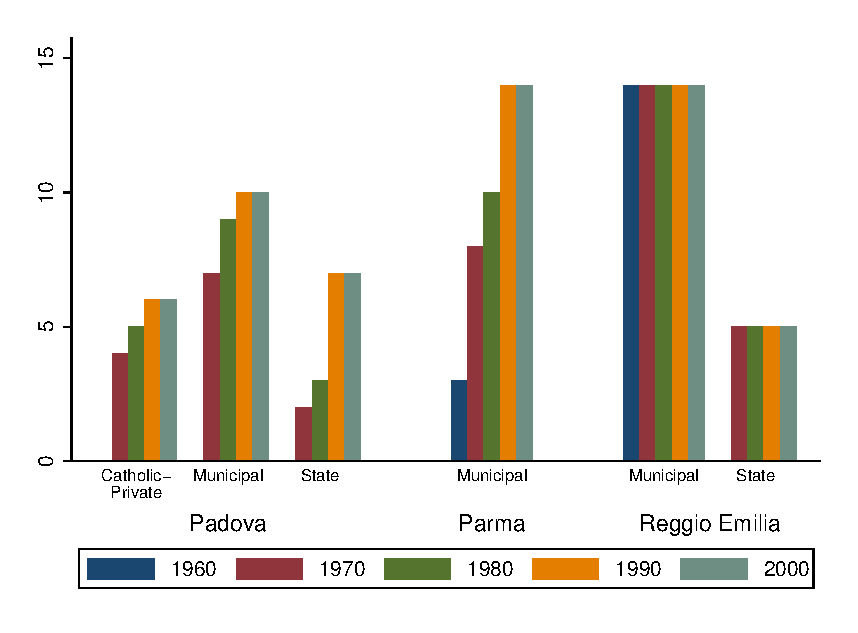
\includegraphics[width=\textwidth]{../../output/aggregateAdministrative.eps}
\end{subfigure}%
~
\begin{subfigure}[b]{0.49\textwidth}
	\caption{Number of Pedagogical Characteristics in Common with the Reggio Approach}\label{fig:agg-ped}
	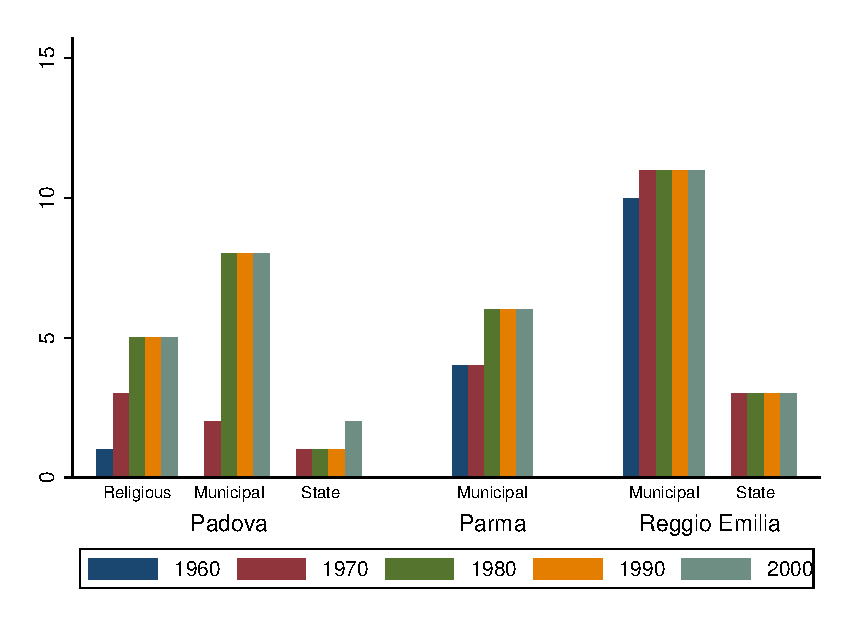
\includegraphics[width=\textwidth]{../../output/aggregatePedagogical.eps}
\end{subfigure}%
\end{center}
\raggedright \footnotesize Note: These graphs show the number of administrative and pedagogical components that each program has in common with the Reggio Approach. We consider 14 administrative components and 16 pedagogical components. Some of the pedagogical components were not present in the Reggio Approach.
\end{figure}

\textbf{[JJH: Can we put in color?] [Typist: Professor, these are currently in color. We will print you a color version tonight.]}
\textbf{[JJH: Please break out the pedagogical components --- summing conceptually different items is a meaningless exercise. Team: This is added below.]}

While the Reggio Approach remains distinctive when considering the combination of its elements, the alternative systems surveyed in our study evolved to include a substantial portion of the elements in Reggio Emilia's municipal system. To better understand which features of the Reggio Approach were adopted by other programs and how they evolved, we document key components by decade and by each system in Tables~\ref{tab:survey-data-atrisk} to~\ref{tab:survey-data-ped}. For the full set of survey items and responses, see Appendix~\ref{sec:survey}.

\begin{table}[H]
	\caption{Policies to Support At-Risk Children and Working Families}\label{tab:survey-data-atrisk}
\centering
\begin{threeparttable}
\begin{tabular}{L{4.5cm} c c c c c c c}
\toprule																	
	&		&	\mc{2}{c}{Reggio Emilia}	&	Parma &	\mc{3}{c}{Padova}	\\	
	\cmidrule(lr){3-4} \cmidrule(lr){5-5} \cmidrule(lr){6-8}
& & Municipal & State & Municipal & Municipal & State & Religious \\
\midrule
\multirow{5}{4.5cm}{Preschools are open 8 hours daily} 	&	1960	&	\checkmark	&		&	\checkmark	&		&		&		\\	
		&	1970	&	\checkmark	&	\checkmark	&	\checkmark	&	\checkmark	&	\checkmark	&	\checkmark	\\	
		&	1980	&	\checkmark	&	\checkmark	&	\checkmark	&	\checkmark	&	\checkmark	&	\checkmark	\\	
		&	1990	&	\checkmark	&	\checkmark	&	\checkmark	&	\checkmark	&	\checkmark	&	\checkmark	\\	
		&	2000	&	\checkmark	&	\checkmark	&	\checkmark	&	\checkmark	&	\checkmark	&	\checkmark	\\	\midrule
\multirow{5}{4.5cm}{Program sites offer extended hours for working families}	&	1960	&	\checkmark	&		&	\checkmark	&		&		&		\\	
		&	1970	&	\checkmark	&	\checkmark	&	\checkmark	&	\checkmark	&		&	\checkmark	\\	
		&	1980	&	\checkmark	&	\checkmark	&	\checkmark	&	\checkmark	&		&	\checkmark	\\	
		&	1990	&	\checkmark	&	\checkmark	&	\checkmark	&	\checkmark	&		&	\checkmark	\\	
		&	2000	&	\checkmark	&	\checkmark	&	\checkmark	&	\checkmark	&		&	\checkmark	\\	\midrule
\multirow{5}{4.5cm}{Priority of enrollment is given to economically disadvantaged families}	&	1960	&	\checkmark	&		&	\checkmark	&		&		&		\\	
		&	1970	&	\checkmark	&	\checkmark	&	\checkmark	&	\checkmark	&		&		\\	
		&	1980	&	\checkmark	&	\checkmark	&	\checkmark	&	\checkmark	&		&		\\	
		&	1990	&	\checkmark	&	\checkmark	&	\checkmark	&	\checkmark	&		&		\\	
		&	2000	&	\checkmark	&	\checkmark	&	\checkmark	&	\checkmark	&		&		\\	\midrule
\multirow{5}{4.5cm}{Priority of enrollment is given to children with disabilities}	&	1960	&	\checkmark	&		&		&		&		&		\\	
		&	1970	&	\checkmark	&	\checkmark	&		&	\checkmark	&	\checkmark	&		\\	
		&	1980	&	\checkmark	&	\checkmark	&		&	\checkmark	&	\checkmark	&		\\	
		&	1990	&	\checkmark	&	\checkmark	&	\checkmark	&	\checkmark	&	\checkmark	&	\checkmark	\\	
		&	2000	&	\checkmark	&	\checkmark	&	\checkmark	&	\checkmark	&	\checkmark	&	\checkmark	\\	\midrule
\multirow{5}{4.5cm}{Priority of enrollment is given to single-parent families}	&	1960	&	\checkmark	&		&		&		&		&		\\	
		&	1970	&	\checkmark	&		&		&	\checkmark	&		&		\\	
		&	1980	&	\checkmark	&		&	\checkmark	&	\checkmark	&		&		\\	
		&	1990	&	\checkmark	&		&	\checkmark	&	\checkmark	&	\checkmark	&		\\	
		&	2000	&	\checkmark	&		&	\checkmark	&	\checkmark	&	\checkmark	&		\\	
\bottomrule	
\end{tabular}	
\end{threeparttable}																
\end{table}

\begin{table}[H]
	\caption{Administrative Practices}\label{tab:survey-data-admin}
\centering
\begin{adjustbox}{width=0.9\textwidth}
\begin{threeparttable}
\begin{tabular}{L{5cm} c c c c c c c}
\toprule																	
	&		&	\mc{2}{c}{Reggio Emilia}	&	Parma &	\mc{3}{c}{Padova}	\\	
	\cmidrule(lr){3-4} \cmidrule(lr){5-5} \cmidrule(lr){6-8}
& & Municipal & State & Municipal & Municipal & State & Religious \\
\midrule
\multirow{5}{5cm}{Parental boards or advisory groups are encouraged as active participants in school culture}	&	1960	&	\checkmark	&		&		&		&		&		\\	
	&	1970	&	\checkmark	&	\checkmark	&	\checkmark	&	\checkmark	&		&	\checkmark	\\	
	&	1980	&	\checkmark	&	\checkmark	&	\checkmark	&	\checkmark	&		&	\checkmark	\\	
	&	1990	&	\checkmark	&	\checkmark	&	\checkmark	&	\checkmark	&		&	\checkmark	\\	
	&	2000	&	\checkmark	&	\checkmark	&	\checkmark	&	\checkmark	&		&	\checkmark	\\ \midrule
\multirow{5}{5cm}{Full-time, degreed Pedagogistas\footnote{In non-Reggio Approach systems, this role is referred to as Educative Coordinator. The job responsibilities of Educative Coordinators do vary across cities and ECE systems.} are hired by the system to oversee professional development for multiple program sites}	&	1960	&	\checkmark	&		&		&		&		&		\\	
	&	1970	&	\checkmark	&		&		&		&		&		\\	
	&	1980	&	\checkmark	&		&		&	\checkmark	&		&		\\	
	&	1990	&	\checkmark	&		&	\checkmark	&	\checkmark	&	\checkmark	&		\\	
	&	2000	&	\checkmark	&		&	\checkmark	&	\checkmark	&	\checkmark	&		\\	\midrule
\multirow{5}{5cm}{Professional development is provided by highly trained educational coordinators to each program site every 1-2 weeks\footnote{In Padova's religious programs, professional development is provided by a mixture of part-time and full-time Educative Coordinators.}}	&	1960	&	\checkmark	&		&		&		&		&		\\	
	&	1970	&	\checkmark	&		&		&		&		&	\checkmark	\\	
	&	1980	&	\checkmark	&		&		&		&		&	\checkmark	\\	
	&	1990	&	\checkmark	&		&	\checkmark	&		&	\checkmark	&	\checkmark	\\	
	&	2000	&	\checkmark	&		&	\checkmark	&		&	\checkmark	&	\checkmark	\\	\midrule
\multirow{5}{5cm}{Full-time Atelierista, or expert in creative visual arts, is staffed at each preschool site and collaborates with classroom teachers to design creative learning activities}
	&	1960	&	\checkmark	&		&		&		&		&		\\	
	&	1970	&	\checkmark	&		&		&		&		&		\\	
	&	1980	&	\checkmark	&		&		&	\checkmark	&		&		\\	
	&	1990	&	\checkmark	&		&		&	\checkmark	&		&		\\	
	&	2000	&	\checkmark	&		&		&	\checkmark	&		&		\\	\midrule
\multirow{5}{5cm}{Kitchen and janitorial staff join educators for professional development}	&	1960	&	\checkmark	&		&		&		&		&		\\	
	&	1970	&	\checkmark	&		&	\checkmark	&		&		&		\\	
	&	1980	&	\checkmark	&		&	\checkmark	&		&		&		\\	
	&	1990	&	\checkmark	&		&	\checkmark	&		&		&		\\	
	&	2000	&	\checkmark	&		&	\checkmark	&	\checkmark	&		&		\\	\midrule
\multirow{5}{5cm}{Scheduled work hours are set aside weekly for teachers to document children's work}	&	1960	&	\checkmark	&		&		&		&		&		\\	
	&	1970	&	\checkmark	&		&		&	\checkmark	&		&		\\	
	&	1980	&	\checkmark	&		&	\checkmark	&	\checkmark	&		&	\checkmark	\\	
	&	1990	&	\checkmark	&		&	\checkmark	&	\checkmark	&		&	\checkmark	\\	
	&	2000	&	\checkmark	&		&	\checkmark	&	\checkmark	&		&	\checkmark	\\	\midrule
\multirow{5}{5cm}{Scheduled hours are set aside weekly for teachers to engage families}	&	1960	&	\checkmark	&		&		&		&		&		\\	
	&	1970	&	\checkmark	&		&	\checkmark	&		&		&	\checkmark	\\	
	&	1980	&	\checkmark	&		&	\checkmark	&		&		&	\checkmark	\\	
	&	1990	&	\checkmark	&		&	\checkmark	&	\checkmark	&		&	\checkmark	\\	
	&	2000	&	\checkmark	&		&	\checkmark	&	\checkmark	&		&	\checkmark	\\	\midrule
\multirow{5}{5cm}{Classrooms are homogeneous in age} 	&	1960	&	\checkmark	&		&		&		&		&		\\	
	&	1970	&	\checkmark	&	\checkmark	&		&		&		&		\\	
	&	1980	&	\checkmark	&	\checkmark	&		&		&		&		\\	
	&	1990	&	\checkmark	&	\checkmark	&		&		&		&		\\	
	&	2000	&	\checkmark	&	\checkmark	&		&		&		&		\\	\midrule
\multirow{5}{5cm}{2 co-teachers for incoming cohorts of 3 year olds. At least 1 teacher stays with the cohort for the next two years to maintain continuity of care}	&	1960	&		&		&		&		&		&		\\	
	&	1970	&	\checkmark	&	\checkmark	&		&		&		&		\\	
	&	1980	&	\checkmark	&	\checkmark	&	\checkmark	&	\checkmark	&		&		\\	
	&	1990	&	\checkmark	&	\checkmark	&	\checkmark	&	\checkmark	&		&		\\	
	&	2000	&	\checkmark	&	\checkmark	&	\checkmark	&		&		&		\\	
\bottomrule
\end{tabular}
\end{threeparttable}		
\end{adjustbox}															
\end{table}

\begin{table}[H]
	\caption{Pedagogical Components}\label{tab:survey-data-ped}
\centering
\begin{adjustbox}{width=\textwidth}
\begin{threeparttable}
\begin{tabular}{L{5.5cm} c c c c c c c}
\toprule																	
	&		&	\mc{2}{c}{Reggio Emilia}	&	Parma &	\mc{3}{c}{Padova}	\\	
	\cmidrule(lr){3-4} \cmidrule(lr){5-5} \cmidrule(lr){6-8}
& & Municipal & State & Municipal & Municipal & State & Religious \\
\midrule
\multirow{5}{5.5cm}{Theories of psychology and early childhood education (e.g. Bloom, Bruner, Gardner, Piaget, Vygotsky) influenced educational approaches}	&	1960	&	\checkmark	&		&		&		&		&		\\	
		&	1970	&	\checkmark	&		&		&		&		&		\\	
		&	1980	&	\checkmark	&		&	\checkmark	&	\checkmark	&		&	\checkmark	\\	
		&	1990	&	\checkmark	&		&	\checkmark	&	\checkmark	&		&	\checkmark	\\	
		&	2000	&	\checkmark	&		&	\checkmark	&	\checkmark	&		&	\checkmark	\\	\midrule
\multirow{5}{5.5cm}{Curriculum emerges through research-based projects with unlimited timelines}	&	1960	&	\checkmark	&		&		&		&		&		\\	
		&	1970	&	\checkmark	&		&		&		&		&		\\	
		&	1980	&	\checkmark	&		&		&	\checkmark	&		&		\\	
		&	1990	&	\checkmark	&		&	\checkmark	&	\checkmark	&		&		\\	
		&	2000	&	\checkmark	&		&	\checkmark	&	\checkmark	&		&		\\	\midrule
\multirow{5}{5.5cm}{Visual arts help children learn}	&	1960	&	\checkmark	&		&	\checkmark	&		&		&	\checkmark	\\	
		&	1970	&	\checkmark	&		&	\checkmark	&		&		&	\checkmark	\\	
		&	1980	&	\checkmark	&		&	\checkmark	&		&		&	\checkmark	\\	
		&	1990	&	\checkmark	&		&	\checkmark	&		&		&	\checkmark	\\	
		&	2000	&	\checkmark	&		&	\checkmark	&		&		&	\checkmark	\\	\midrule
\multirow{5}{5.5cm}{Teachers document children's learning}	&	1960	&	\checkmark	&		&		&		&		&		\\	
		&	1970	&	\checkmark	&		&		&	\checkmark	&		&	\checkmark	\\	
		&	1980	&	\checkmark	&		&	\checkmark	&	\checkmark	&		&	\checkmark	\\	
		&	1990	&	\checkmark	&		&	\checkmark	&	\checkmark	&		&	\checkmark	\\	
		&	2000	&	\checkmark	&		&	\checkmark	&	\checkmark	&	\checkmark	&	\checkmark	\\
	\bottomrule
\end{tabular}	
\end{threeparttable}	
\end{adjustbox}															
\end{table}					

These results indicate that the main components of the Reggio Approach practiced in non-Reggio Approach programs include (i) the engagement of families in school management; (ii) administrative practices for at-risk children and working families, and; (iii) the use of highly trained educational coordinators to routinely support professional development. In general, non-Reggio Approach programs are similar to each other, and different from the Reggio Approach, in providing religious teaching and following a daily program designed to guide children in acquiring knowledge of specific concepts. 

The general trend is consistent with the explanation that common influences were operating at the onset of these programs. Additionally, survey results mildly support a spillover story of Reggio Approach features into other early childhood programs as treatment effects are found only for the oldest cohorts. We more closely examine these patterns in each of the other early childhood systems below. 

\textbf{[JJH: How can a survey reveal spillovers or not? Team: We cannot definitely state there is spillover. The text has been edited to reflect this.]} 

\subsection{State Preschools}

Over time and across cities, each cohort in our sample had access to different numbers of state preschools. Further, those who enrolled in state programs experienced varying early childhood curricula and administrative practices.

In 1968, Law 444 ensured access to a system of free, state preschool for all families that applied.\footnote{In state programs, parents pay only for meals and transportation.} Law 444 is considered a key shift in Italian policies for early childhood as it legitimized state involvement in public and private education for ages 3-6 years \citep{Hohnerlein_2009_Paradox-Public-Preschools}. \textbf{[JJH: Discuss features of the 1968 literature. Sylvi: This is added.]} By Law 444, the state was responsible for school construction, materials and equipment. Municipalities, however, were mandated to maintain state preschools and fund the salaries of an all-female teaching staff under 35 years of age, with a vocational diploma from a 3-year high school \citep{OECD_2001_Italy-Country-Note}.\footnote{Later reforms transferred constructions costs from the state to municipalities, allowed men to work as early childhood educators, and required laureate degrees.} 

By providing funds only to construct state preschools where local demand was not met by existing non-state systems such as municipal and religious schools, Law 444 resulted in disparate numbers of state preschools in Reggio Emilia, Parma, and Padova for each of the cohorts in our evaluation \citep{Hohnerlein_2009_Paradox-Public-Preschools}. Historical records indicate that state preschools first appeared in Reggio Emilia and Padova between 1973-1975 \citep{Padova-Admin-Data_1964-2011,Reggio-Admin-data_1966-2006,Reggio-Annual-Journals_1994-2011}. In contrast to other areas of Italy where the state is currently the largest provider of preschool education, enrollment in Reggio Emilia, Parma, and Padova's state preschools is historically lower than enrollment in municipal and religious preschools. Although the state does not offer infant-toddler childcare, it regulates and subsidizes these programs through regional governments per Law 1044 enacted in 1971.

\textbf{[JJH: What is municipal and what is municipal preschool? Team: we use ``system'' to indicate the network of infant-toddler and preschool sites. We have clarified the above sentence to read preschool instead of program.]}

Reports suggest that periodic policy reforms and improved guidelines for state preschools (Orientamenti) were influenced by municipal programs from the region of Emilia Romagna, including Reggio Emilia, Milan, and Pistoia \citep{OECD_2001_Italy-Country-Note}. In particular, revised mandates for lower teacher-child ratios, and higher qualifications for teacher education are proposed as key quality indicators associated with diminishing disparities in state and non-state programs by the end of the 20th century \citep{Hohnerlein_2015_Development-and-Diffusion}. For example, between 1969 and 1980 for the age-40 and age-30 cohorts, teacher-child ratios were very low ranging from 1:17-30 children aged 3-6 years, and teacher education took place in religious institutions.\footnote{In contrast, teacher-child ratios in the Reggio Approach were 2:25-30 from 1972 forward.} After 1991, attendees of state preschools in the adolescent and child cohorts experienced better physical accessibility to schools, a 1:12-13 teacher-child ratio (equivalent to that of the Reggio Approach), and teachers who were trained in universities \citep{Hohnerlein_2015_Development-and-Diffusion}. The two younger cohorts further benefitted from 1991 revisions to Orientamenti stressing the contributions of social relationships for cognitive development and the value of communication for home-school relationships \citep{OECD_2001_Italy-Country-Note}. Six content goals for early childhood education and their associated skill-sets were also outlined by the state for the first time, including (i) the body and movement; (ii) language and speech; (iii) space, order, and measure; (iv) things, time, and nature; (v) messages, forms and media, and; (vi) the self and other \citep{Orientamenti_1991_Scuola-Materna}.\footnote{In the Reggio Approach, specific skill-sets to be acquired are explicitly not stated as a requirement for early childhood education.} The methods, however, by which these concepts should be taught were not stated in order to enable autonomy and flexibility at the school-level.

In theory, mandated administrative operations and policies for state preschools should be consistent throughout Italy. Indeed, survey results indicate that administrative operations for state preschools in Padova are similar to state preschools in Reggio Emilia, with two interesting exceptions. In Padova, parents must pay for extras such as field trips, whereas in Reggio Emilia, field trips for children in state preschools are funded by the municipality. Padova's state preschools report staffing full-time educational coordinators to provide professional development for state teachers from the 1990s forward, which is a feature of the Reggio Approach. In Reggio Emilia, however, state preschools do not report the hiring of full-time educational coordinators. 

Survey results indicate that several administrative features of state preschools are different from the Reggio Approach (and from municipal programs in Parma and Padova). State preschools do not hire a full-time expert in the creative arts and do not set aside time for teachers to engage families. State preschools do not offer extended hours to working families. And, at 30 hours per week, state teachers work 6 hours less than their municipal counterparts. With reduced teaching hours and reduced full-time staff, children in state preschools spend more hours with only one teacher than do children in Reggio Approach preschools (see Appendix Table \ref{tab:programoperation}). 

In support of a spillover argument, state preschools in Reggio Emilia implement two Reggio Approach practices that are not offered in Padova's state preschools. These practices include the use of homogeneous-aged classrooms and the focus on continuity of care for children and families by keeping at least one teacher with each cohort for three years. Overall, however, pedagogy in state preschools of both Reggio Emilia and Padova  supports children's learning differently than in the Reggio Approach. State preschools (like religious preschools in all three cities) emphasize moral development, national patriotism and family values. Survey results further indicate that teaching in state preschools (like municipal schools in Parma and Padova), is influenced by different academic theories, includes religious teaching, and use programmed daily activities to guide children in learning of specific concepts (see Appendix Tables~\ref{tab:programoperation} to \ref{tab:environ-features}). 

Our study evaluated whether these additional features of Reggio have any benefits. They appear not to. \textbf{[Team: We propose the following revision: Our study evaluated whether features of the Reggio Approach not employed by state preschools were effective in benefitting individuals sufficiently to cause significant improvement in outcomes relative to individuals who did not receive the Reggio Approach. They appear not to.]}

\subsection{Religious Early Childhood Programs}

The Catholic Church is the oldest early childhood provider in Italy, offering both religious training and charitable social services for disadvantaged children since the 19th century \citep{OECD_2001_Italy-Country-Note}. All five cohorts in our evaluation had access to religious programming for ages 3-6 years; of the three cities, Padova offers the largest number of religious preschools. Until the 1990s, religious sites in Reggio Emilia, Parma, and Padova did not offer educational infant-toddler programs. At some sites in each municipality, the adolescent cohort had access to several months of transitional programming for children over 24 months of age; from 12 months of age, the child cohort had access to infant-toddler childcare \citep{Malizia-Cicatelli_2011_BOOK_Catholic-School,CEHD_2016_Historical-Analysis}.

To provide administrative support for independent religious schools, local federations began to assemble throughout Italy in the mid-1970s. Religious preschools within the cities of Reggio Emilia, Parma, and Padova could join a city-level federation that supported administrative operations. \textbf{[JJH: Churches? What's a site? Church? Sylvi: Correct. JJH: What is the content of the program? Sylvi: We revised the text below to reflect educational goals for equitable religious schools for cohorts after 1997-2000. Before then, none are reported in the literature nor in our survey. For all of our cohorts, however, there is no stated pedagogical approach to achieve these stated goals that we can ascribe to individual religious sites nor to local federations such as the use of project-based active-child learning or teacher-initiated activities.]} In contrast to the Reggio Approach, however, religious schools within the same local federation are not mandated to implement a unified pedagogy for preschool education; in this sense, the Church supports the autonomy of individual religious sites to determine their own methodologies \citep{Malizia-Cicatelli_2011_BOOK_Catholic-School}. 

Following a 1997 policy that enabled state funding for non-state programs meeting national guidelines for early childhood, the Catholic Church undertook significant efforts to quantify and achieve equitable program quality in religious schools for all ages. At some time after 1997, we can expect that policies and educational goals in religious preschools seeking equitable status began to reflect state laws and guidelines. Indeed, after 2000, the Church reports efforts throughout Italy to replace religious educators with secular teachers trained in higher institutions and reducing teacher-child ratios to reflect national standards \citep{Malizia-Cicatelli_2011_BOOK_Catholic-School}. Religious programs that succeeded in achieving equitable status would thus, like state preschools, reflect the influence of municipal systems in the Province of Emilia Romagna, including Reggio Emilia \citep{Hohnerlein_2009_Paradox-Public-Preschools,OECD_2001_Italy-Country-Note}. 

Our study does not collect site-level data that would confirm which religious early childhood programs achieved equitable status nor the timing of such a shift; we cannot thus determine the extent to which adolescents and children in our evaluation may have attended equitable religious schools. Survey results indicate that the majority of religious sites in all three municipalities achieved equitable status during the 2000s. We thus estimate that the child cohort likely had access to equitable religious preschools; those children who enrolled experienced a program of similar quality as children who enrolled in state preschools. We further note that parents of the youngest cohort who chose equitable religious preschools were eligible for subsidized tuition on a sliding-scale basis; prior to 2000, tuition and fees for religious preschool in all three cities was more expensive than the cost of attending municipal and state preschools.

Survey results for religious preschools are available for Reggio Emilia for the 2000s, reflecting only the experience of the child cohort in our study. In support of a spillover story, religious preschools in Reggio Emilia are the only other system we survey that do not implement daily activities to guide children in acquiring specific content knowledge. Religious preschools in Reggio Emilia, further like the Reggio Approach and unlike religious preschools in Padova, hire full-time educational coordinators, keep at least one of two co-teachers with each cohort for three years to ensure continuity of care, and maintain homogenous-aged classrooms.\footnote{Survey results indicate that homogenous-aged classrooms are only practiced in Reggio Emilia; all systems in Parma and Padova maintain mixed-age classrooms.} Religious preschools in Reggio Emilia, like the Reggio Approach, also offer extended hours for working families; include an atelier, in-house kitchen, and emphasize natural materials and open spaces; encourage parents to serve on school boards; hire full-time educational coordinators to oversee professional development; are influenced by the same academic theories; employ project-based learning with flexible timelines; set weekly hours for teachers to engage families and document children's work; and incorporate fine arts to support children's learning. 

Of all the systems we survey, only Padova's religious early childhood system reports that Malaguzzi's educational practices shaped their daily program; this influence is reported only for some religious sites starting in the 2000s. Regardless, survey evidence suggests that religious preschools in Padova share the following practices with the Reggio Approach: from the 1970s, schools were open 8 hours and extended hours were available for working parents; parents were encouraged to serve on school boards and weekly time was set aside for teachers to engage families. From the 1980s, teachers began to document children's work and school environments included an atelier. From the 1990s, Padova's religious schools prioritized enrollment for children with disabilities. 

Unlike the Reggio Approach, pedagogy in both systems include religious teaching; an emphasis on moral development, national patriotism and family values, and; the influence of Agazzi, Froebl and Montessori. Only Padova's religious preschools follow a daily program to guide children in learning specific concepts (see Appendix Table \ref{tab:educ-program}). Municipal archives from 1970 indicate that children aged 3-6 years enrolled in Padova's religious preschools experienced one teacher for 34-44 children \citep{Padova-Admin-Data_1964-2011}. 

Unlike the Reggio Approach, religious preschools in Reggio Emilia and Padova do not prioritize the enrollment of children from economically disadvantaged families (see Appendix Table \ref{tab:administrative-atrisk}).  In Reggio Emilia only, religious preschools are not open 8 hours daily; do not hire full-time atelieristas; do not include cooks and janitors in teacher trainings, and; do not provide teachers with supervision and training on a biweekly basis. These components appear to have no effects for the outcomes that we study.

\subsection{Municipal Early Childhood Systems in Parma and Padova}

\textbf{[JJH: This section is very weak and hurts the paper. Sylvi: The following section has been revised.]}

Survey results, reports, and interviews indicate that the municipal systems in Parma and Padova both grow more similar over time to the Reggio Approach. From their inception, the three municipal systems share many features including a strong emphasis on the provision of high quality programming for infant-toddler centers \citep{Ghedini_2001_Ital-Natl-Policy}. From the 1970s forward, each city invested in staffing municipal schools for 8 hours daily, extended hours for working families, and prioritized enrollment for low-income families. Each city emphasized family participation in school management. From the 1980s forward, all three municipal school environments featured an atelier, in-house kitchens, open spaces, and the use of natural lighting and materials. Furthermore, educational approaches were influenced by the same academic theories of psychology and education. From the 1990s forward, all cities prioritized enrollment for children with disabilities \footnote{In Padova, prioritized enrollment for children with disabilities began in the 1970s.} and included project-based learning as a teaching method.

Of the two cities, Parma's municipal system is more similar in policy and administration to that of Reggio Emilia, sharing the same approach from the 1990s. For example, Parma reports that administrative operations, weekly scheduled hours to engage families, and professional development for teachers began to appear in the mid-late 1970s.\footnote{In Padova, professional development for municipal early childhood staff began in the mid-1980s \citep{Becchi-Ferrari_1990_Pub-Inf-Centres-Italy}.} From the mid-late 1980s, Parma focused on improving management of infant-toddler centers to support the varying needs of working parents. 

From a pedagogical perspective, however, survey results suggest that off all the programs we study, municipal preschools in Padova is more consistently similar to the Reggio Approach. In Padova, teachers began to document children's learning in the 1970s. By the 1980s, fine arts specialists were hired to support creative learning activities. 
\textbf{[JJH: It is only in the 2000s. What is the evidence? Sylvi: We have added content from earlier decades.]} 

Where the Reggio Approach and the municipal systems in Parma and Padova differ is in the application of psychological theories to pedagogical methods. In both Parma and Padova's municipal systems, classrooms are heterogenous in age and religious instruction is provided. In contrast to the progressive Reggio Approach where content knowledge is secondary to creative expression, daily activities in the municipal preschools of Parma and Padova follow a program to guide children in learning specific concepts such as communication, culture, order, measure, space, time, nature, self, and other. In Padova, cognitive development is emphasized, teaching includes direct-instruction, and children complete worksheets as a learning activity \citep{CEHD_2016_Historical-Analysis}. 

\textbf{[JJH: Such as? Sylvi: The program concepts are intentionally vague in order to be actualized at the individual school-level, similar to Head Start. (In contrast, in Reggio, chosen concepts are not pre-determined but follow the child's lead.)]} \textbf{[JJH: Why inconsistent?] [Sylvi: Apologies, I'm unsure what inconsistency you refer to.] [JJH: This has to stop. It's obvious what I said. Knowing order, space, time, etc. is not inconsistent with Reggio. There is no head to head comparison. It looks like Sylvi swallowed Reggio propaganda hook, line, and sinker. Sylvi: I have revised the text throughout and in the summary below to better clarify the progressive model implemented in Reggio as reported by many visiting scholars since the 1970s. I fully agree that knowing specific concepts is not inconsistent with Reggio, and predict that any child who wanted to learn them would be supported. I value your feedback on the revisions.]}.

Overall, relative to Reggio Emilia, investment in municipal early childhood programs and services for ages 0-6 by Parma and Padova occurred approximately 10 years and 15 years later, respectively. In considering selection into different systems by families in each city, we note that Parma and Padova each provided fewer municipal infant-toddler centers and preschools from the 1960s forward. We further note that enrollment is highest in the municipal preschools of Reggio Emilia and Parma, whereas in Padova, it is secondary to enrollment in religious preschools \citep{Padova-Admin-Data_1964-2011,Reggio-Admin-data_1966-2006,Reggio-Annual-Journals_1994-2011}. 

For additional information, see (see Appendix Tables~\ref{tab:programoperation} to \ref{tab:environ-features}). 

\subsection{Summary}

As a whole, the Reggio Approach is not unique compared to other early childhood systems in Reggio Emilia and in neighboring cities of Northern Italy. It appears, however, that the state, religious, and municipal programs we study do not incorporate Reggio Approach practices that reflect Dewey's progressive model. This theory of education prioritizes the process of learning over the learning of specific content. Accordingly, the Reggio Approach explicitly does not define skills that children must acquire and demonstrate during early childhood. Instead, Reggio Emilia's municipal model of progressive early childhood education endorses community activism, creativity, and expression by using language and fine arts as mechanisms for learning. 
%Add cite for no empirical evaluations of Dewey's model? Waiting for Carolyn Edwards...

The evidence presented here supports the finding of more significant outcomes for the age-40 cohort than the age-30 cohort, and fewer differences for adolescents and children in comparisons between programs. 


\section{Research Design}
\label{sec:data}
\subsection{The Selection of Cities}

We survey cohorts of individuals educated in Parma, Padova, and Reggio Emilia. Parma and Padova are similar to Reggio Emilia in terms of geography, population, and socio-economic structure, but they do not have the full Reggio Approach available.\footnote{Other Italian cities were also considered, notably Brescia, Livorno, Modena, Perugia, Piacenza, Prato, and Ravenna. Parma and Padova were the two cities that had social and economic characteristics most similar to Reggio Emilia and were geographically close.}

The cities are in close geographic proximity with Reggio Emilia, which may contribute to the plausibility of spillover effects. Parma is in the same administrative region of Emilia-Romanga. They have similar populations as seen in Figure~\ref{fig:population}. Although the population in Padova is larger than in Parma and Reggio Emilia, the trends are similar across time. The similarity in trends can also be seen in comparing the migration rates among the three cities (Figure~\ref{fig:emigr-immigr}). Although emigration rate is highest in Padova and net migration rate is highest in Reggio Emilia for most of the years, general trends in emigration and immigration are similar in all cities. Levels of foreign immigration are almost identical in the three cities.

The similarities between the cities are also seen in economic terms. Reggio Emilia has an average per-capita income of 25,226 euros, Parma of 28,437, and Padova of 29,915 in 2011 \citep{Comuni-Italiani_2017_Redditi-Ipref-per-Regione-2011}. Other economic information, such as unemployment, is similar across the cities as well. We present additional information on the three cities in Appendix~\ref{sec:data-app}.

\begin{figure}[H]
      \begin{center}
        \begin{subfigure}[t]{0.49\textwidth}
          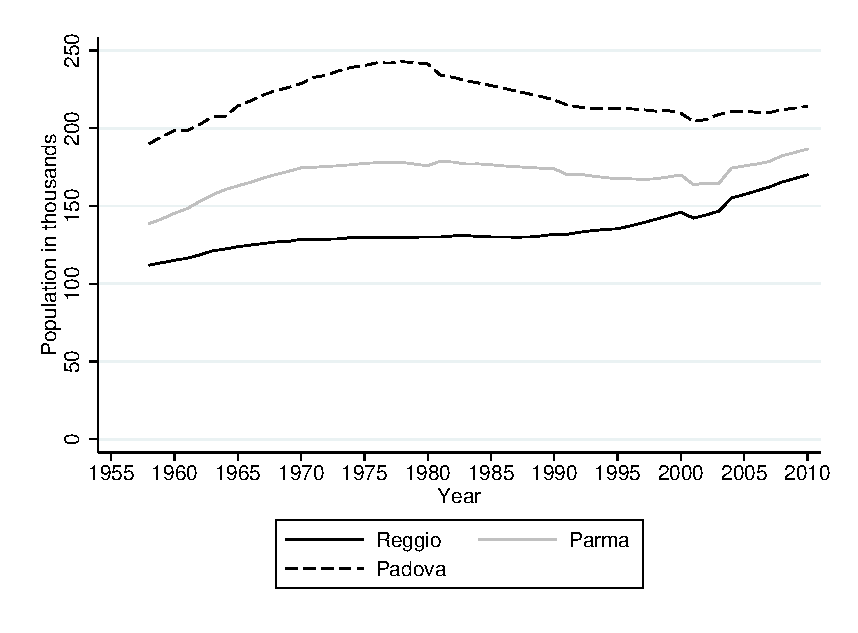
\includegraphics[width=\textwidth]{../../output/image/population.eps}
\caption{Population}
        \end{subfigure}
        \begin{subfigure}[t]{0.49\textwidth}
          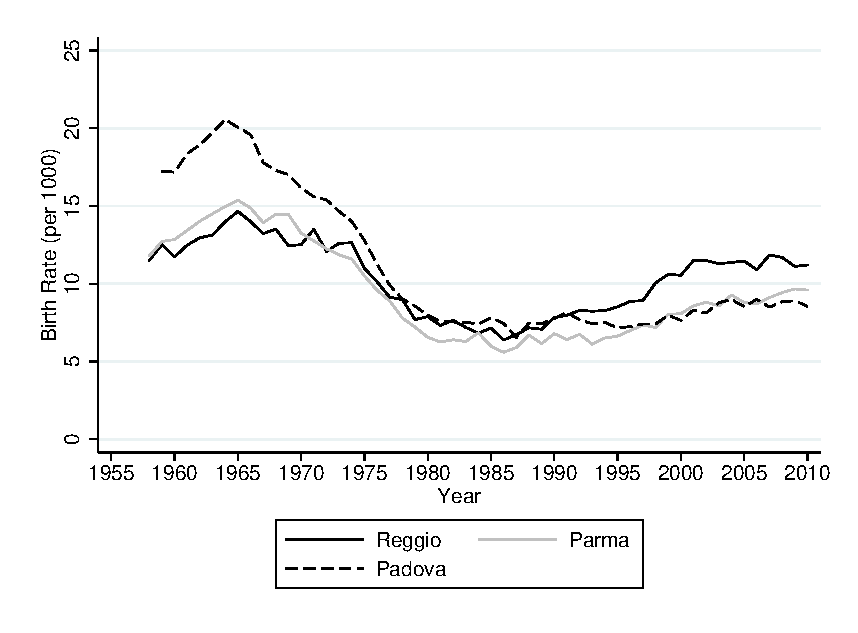
\includegraphics[width=\textwidth]{../../output/image/birth_rate.eps}
 \caption{Birth Rate}
        \end{subfigure}
        \begin{subfigure}[t]{0.49\textwidth}
          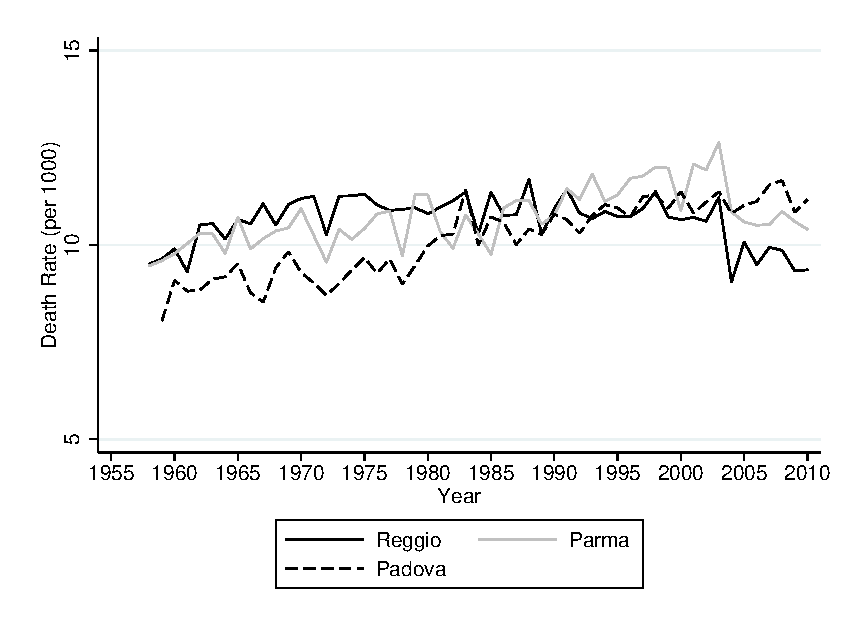
\includegraphics[width=\textwidth]{../../output/image/death_rate.eps}
        \caption{Death Rate}
        \end{subfigure}
        \begin{subfigure}[t]{0.49\textwidth}
          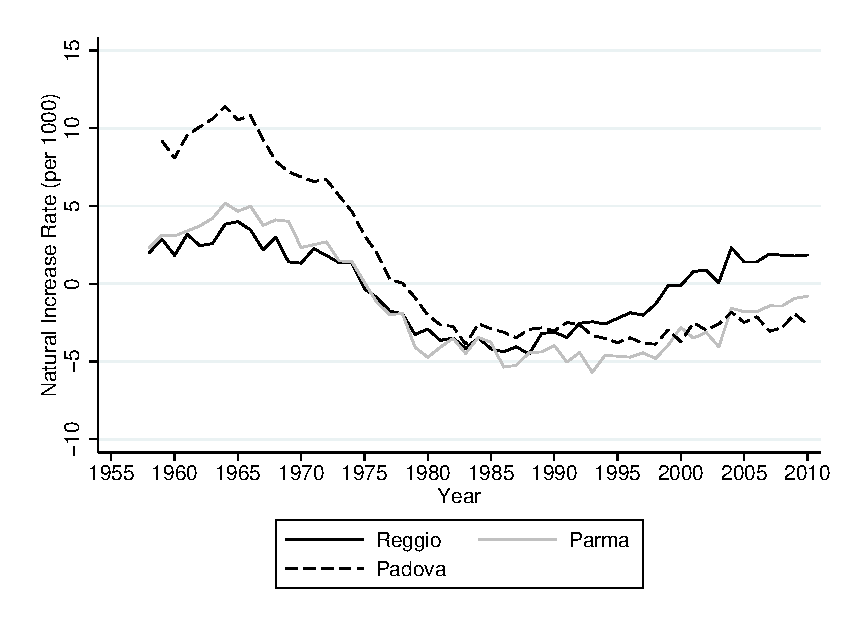
\includegraphics[width=\textwidth]{../../output/image/naturalinc_rate.eps}
            \caption{Natural Rate of Increase}
        \end{subfigure}
      \caption{Population Statistics}  \label{fig:population}
      \end{center}
      \raggedright Note: See Appendix~\ref{sec:data-app} for more information on these data and the sources.
    \end{figure}

\begin{figure}[H]
      \begin{center}
        \begin{subfigure}[t]{0.49\textwidth}
          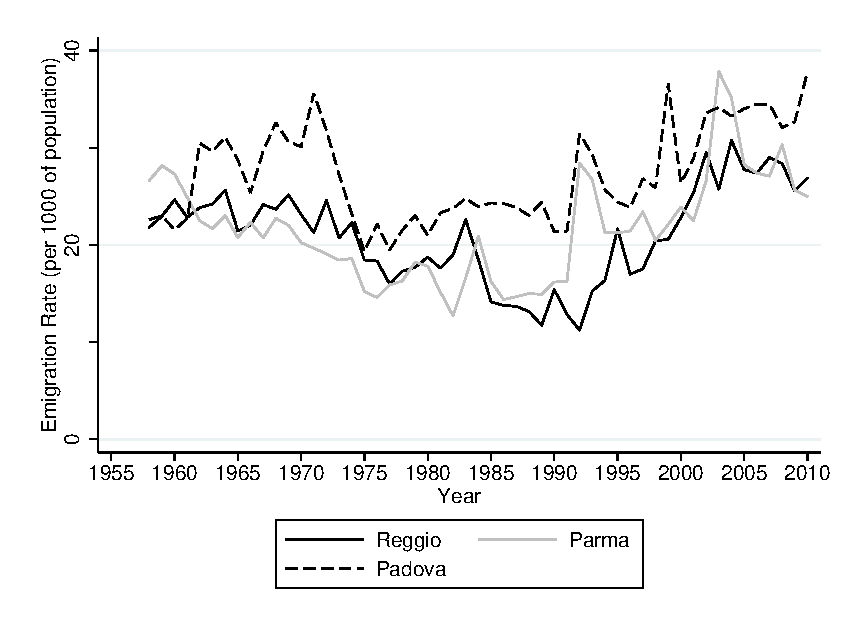
\includegraphics[width=\textwidth]{../../output/image/emigration.eps}
            \caption{Emigration}
        \end{subfigure}
      \begin{subfigure}[t]{0.49\textwidth}
        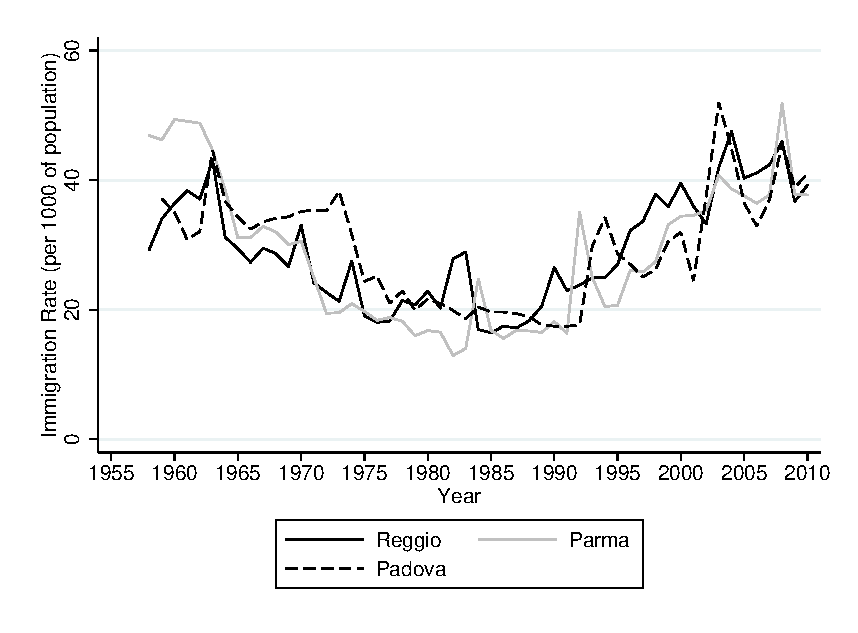
\includegraphics[width=\textwidth]{../../output/image/immigration.eps}
        \caption{Immigration}
      \end{subfigure}
	 \begin{subfigure}[t]{0.49\textwidth}
          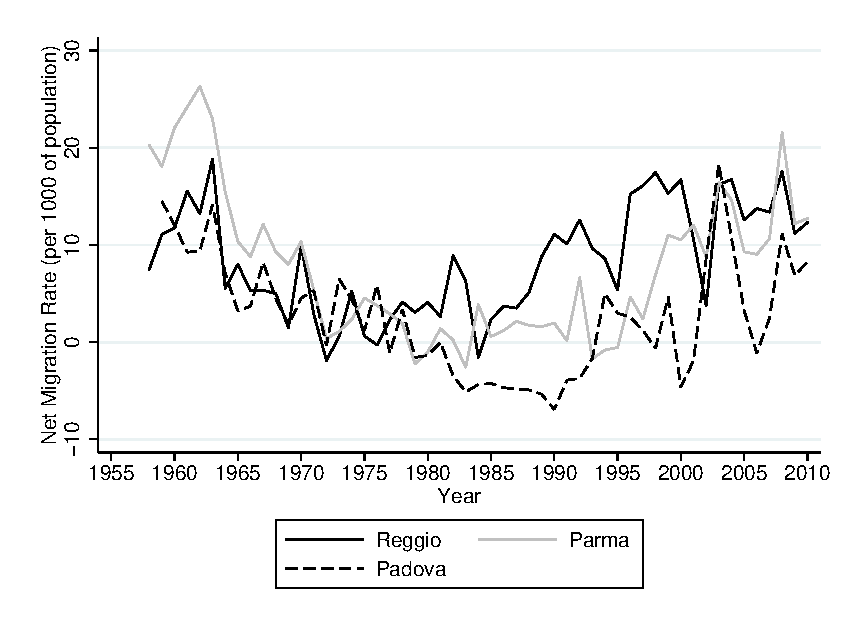
\includegraphics[width=\textwidth]{../../output/image/netmigration.eps}
\caption{Net Migration}
        \end{subfigure}
        \begin{subfigure}[t]{0.49\textwidth}
          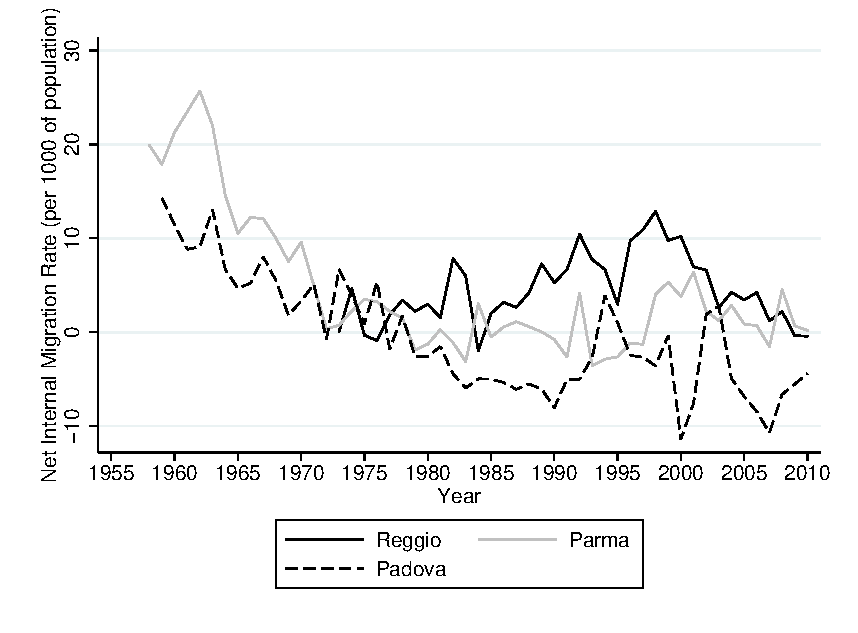
\includegraphics[width=\textwidth]{../../output/image/netinternalmig.eps}
 \caption{Net Internal Migration}
        \end{subfigure}
        \begin{subfigure}[ht]{0.48\textwidth}
          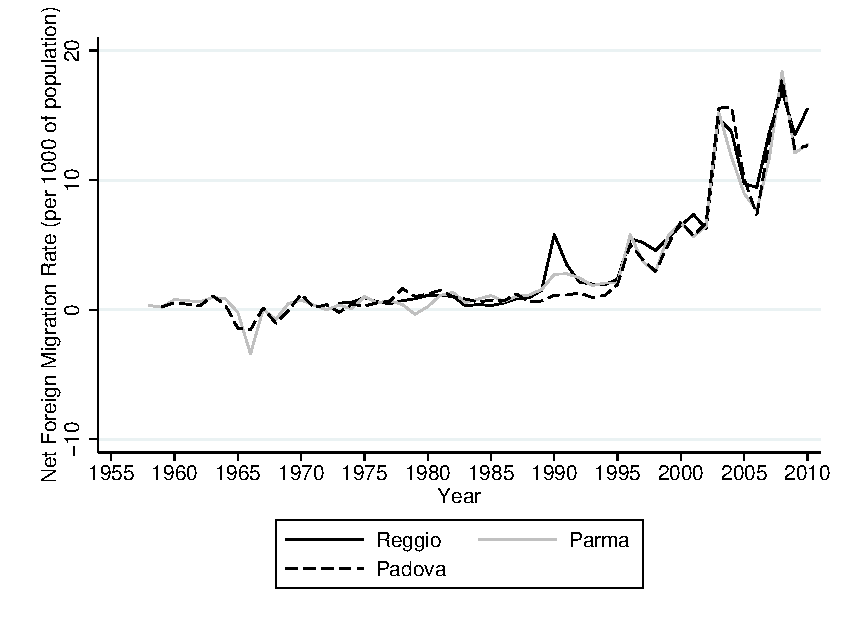
\includegraphics[width=\textwidth]{../../output/image/netforeignmig.eps}
        \caption{Net Foreign Migration}
        \end{subfigure}
      \caption{Migration Statistics}  \label{fig:emigr-immigr}
      \end{center}
         \raggedright  Note: See Appendix~\ref{sec:data-app} for more information on these data and the sources.
    \end{figure}

We summarize the main population statistics in Table~\ref{tab:pop-summary-stat} in which we present the mean and standard deviations of the population, birth rate, death rate, and net migration across years. We compare the means in Parma and Padova to those in Reggio Emilia. Parma and Padova have significantly larger populations.

    \begin{table}[H]
    \centering
    \caption{Summarizing Population Statistics Across Years} \label{tab:pop-summary-stat}
    \begin{threeparttable}
	
	\begin{tabular}{l c c c}
\toprule
&	Reggio Emilia & Parma & Padova \\
\midrule
Population	& 134,459.6 &   \textbf{170,335} &  \textbf{219,161.2}   \\
			& (13,413.67) & (10,104.85)& (13,474.66)   \\
Birth rate & 		10.38 &9.36  & 	11.08 \\
	(per 1,000)	&		(2.33) & (3.02) & (4.55) \\
Death rate &  10.62 &  10.74 & \textbf{10.13} \\
	(per 1,000)	& (0.63) & (0.74) & (095) \\
Net migration & 8.40 &  7.38 & \textbf{2.68} \\
	(per 1,000)		& (5.63) & (7.36) & (5.96) \\
\bottomrule
\end{tabular}


\begin{tablenotes}
\item \footnotesize Note: This table summarizes the average of population statistics across available years by city. A bolded mean indicates that it is significantly different from Reggio Emilia at least at the 0.05 level. Standard deviations are reported in parentheses. See Appendix~\ref{sec:data-app} for more information on these data and the sources.
\end{tablenotes}
\end{threeparttable}
\end{table}

Although the three cities are similar, Parma has more in common with Reggio Emilia than does Padova. This is the case for population indicators, such as those in Table~\ref{tab:pop-summary-stat}, but also for indicators of social setting. An example of this is seen in Appendix~\ref{sec:data-app} which has the proportion of votes for different parties between 1953 and 1993. In both Reggio Emilia and Parma, more votes went towards the Communist Party, whereas Padova had a higher proportion of votes going towards the Christian Democrats.

The proximity and comparability of the three cities are useful for standardizing on background variables. However, it may compromise sharp comparisons of the effectiveness of alternative school systems given the similarities in preschool features and commonality of cultural influences.
	

\subsection{The Survey Data Collection}

Respondents were sampled from the population registries of the cities based on their year of birth. The sample was then restricted to those individuals living in the same city in which they were raised. All cohorts, except the youngest one, are restricted to individuals who are Italian citizens. In contrast, the youngest cohort includes an oversampling of immigrant children.\footnote{In the adult cohorts there was no immigrant who was preschool age in the same school in which they live. In the adolescent cohort, the number was immigrant born was extremely small.} The sample from Reggio Emilia, across all cohorts, includes an oversampling of those who attended municipal schools, as this is our treatment group.

Of the reference sample, 7,176 individuals were randomly selected. Of these, 4,019 completed interviews, resulting in a response rate of 56\%.\footnote{We have very limited information on those who refused. Thus, we are unable to adjust for this high non-responsive rate.} Table~\ref{tab:sample-response} provides an overview of the birth years for the different cohorts, the counts of the full sample, and the response rate. The most common reasons for non-response were that nobody was home when the surveying agency solicited and sharp refusals.

\begin{table}[H]
\centering
\begin{threeparttable}
	\caption{Description of the Full Sample and Response Rates}\label{tab:sample-response}
	\begin{tabular}{l c c c c c c}
\toprule
Cohort & Birth year(s) & Age at interview & Reggio Emilia & Parma & Padova & \textbf{Total} \\			
\midrule
\textbf{Children} &  &  &  & &  &  \\ 
\quad Italians & 2006 & 7 & 311 & 291& 278 & 880 \\
			&&	& \textit{50.0\%} &  \textit{62.7\%} &  \textit{50.0\%} &  \textit{53.6\%} \\
\quad Migrants & 2006 & 7 & 110 & 58 & 113 & 281 \\
			&& 	&  \textit{53.1\%} &  \textit{49.2\%} &  \textit{63.1\%} &  \textit{55.8\%} \\
\textbf{Adolescents} & 1994 & 19 & 300 & 254 & 282 & 836 \\
			&& 	&  \textit{57.1\%} &  \textit{58.5\%} &  \textit{55.5\%} &  \textit{57.0\%} \\
\textbf{Adults 30s} & 1980-1981 & 32 & 280 & 251 & 251 & 782 \\
			&& 	&  \textit{58.3\%} &  \textit{58.2\%} &  \textit{57.4\%} &  \textit{57.9\%} \\
\textbf{Adults 40s} & 1969-1970 & 43 & 285 & 254 & 252 & 791 \\
			&& 	&  \textit{59.3\%} &  \textit{56.3\%} &  \textit{53.8\%} &  \textit{56.0\%}\\
\textbf{Adults 50s} & 1954-1959 & 54-60 & 200 & 103 & 146 & 449 \\
			&& 	&  \textit{52.2\%} &  \textit{63.6\%} &  \textit{55.6\%}  &  \textit{55.6\%}\\
\midrule
\textbf{Total}	& 				& & 1,486 & 1,211 & 1,322 & 4,019 \\
			&&				& \textit{55.1\%} &  \textit{58.8\%} &  \textit{55.0\%} & \textit{56.0\%} \\
\bottomrule
\end{tabular}

\begin{tablenotes}
\footnotesize
Note: The response rates for each city and cohort are in italics. They are the the ratio of interviews to total valid contacts. Valid contacts are the sum of: completed interviews, sharp refusal, no person present, talked with a relative, left paper questionnaire but never returned, interview began but not completed. The age at interview is an approximation given there is some variation in the interview date and birth year within each cohort. In analysis, we combine the Italian and migrant subsamples of the child cohort and control for migrant status.
\end{tablenotes}
\end{threeparttable}
\end{table}

Tables~\ref{tab:sample-asilo} and \ref{tab:sample} provide a detailed tabulation of the sample by city, cohort, and school type for both infant-toddler care and preschool attendance. They show that the number of people who do not attend any preschool and infant-toddler center decreases over time. Whereas the majority of individuals from the age-50 cohort did not attend any infant-toddler care or preschool, there are few such cases in the child and adolescent cohorts. These tables also show that the proportion of individuals attending municipal infant-toddler centers and preschools is higher in Reggio Emilia than in the other cities.\footnote{This is due to the construction of the sample.} Note that the Reggio Approach preschools were not available for the age-50 cohort. \textbf{[JJH: We need a definition of muni-affiliated -- not previously discussed or defined.][Team: We added the definition of muni-affiliated in the background section.]}

\begin{table}[H]
\centering
\scalebox{0.85}{
\begin{threeparttable}
	\caption{Tabulation of Infant-Toddler Care Attendance by Cohort, City, and School Type}\label{tab:sample-asilo}
	\begin{tabular}{l*{7}{c}}
\toprule
		&	\mc{6}{c}{Reggio Emilia: 1,486}													\\	\midrule
		&	None	&	Muni	&	Reli	&	Priv	&	Muni-Affi	&	Other	\\	\midrule		
\textbf{Children	}&		&		&		&		&		&		\\	
\quad Italians	&	115	&	109	&	28	&	6	&	51	&	0	\\			
\quad Migrants		&	58	&	24	&	2	&	0	&	20	&	3	\\			
\textbf{Adolescents}		&	129	&	112	&	10	&	3	&	36	&	3	\\			
\textbf{Adults 30s}		&	210	&	53	&	2	&	3	&	1	&	7	\\			
\textbf{Adults 40s}		&	241	&	31	&	0	&	0	&	0	&	5	\\			
\textbf{Adults 50s}		&	194	&	0	&	1	&	0	&	0	&	1	\\	\midrule		
		&	\mc{6}{c}{ Parma: 1,211}											\\	\midrule		
		&	None	&	Muni	&	Reli	&	Priv	&	Muni-Affi	&	Other	\\	\midrule	
\textbf{Children}&		&		&		&		&		&		\\		
\quad Italians		&	98	&	99	&	7	&	15	&	48	&	21	\\			
\quad Migrants		&	24	&	23	&	1	&	0	&	9	&	1	\\			
\textbf{Adolescents}		&	126	&	74	&	10	&	11	&	25	&	2	\\			
\textbf{Adults 30s}		&	187	&	31	&	8	&	6	&	11	&	4	\\			
\textbf{Adults 40s}		&	222	&	0	&	2	&	0	&	10	&	16	\\			
\textbf{Adults 50s}		&	85	&	0	&	4	&	0	&	0	&	13	\\	\midrule		
		&	\mc{6}{c}{Padova: 1,322}											\\	\midrule		
		&	None	&	Muni	&	Reli	&	Priv	&	Muni-Affi	&	Other	\\	\midrule		
\textbf{Children}&		&		&		&		&		&		\\		
\quad Italians		&	143	&	48	&	26	&	40	&	19	&	1	\\			
\quad Migrants		&	57	&	44	&	3	&	5	&	0	&	1	\\			
\textbf{Adolescents}		&	209	&	52	&	8	&	0	&	6	&	1	\\			
\textbf{Adults 30s}		&	220	&	19	&	5	&	3	&	0	&	0	\\			
\textbf{Adults 40s}		&	225	&	0	&	7	&	0	&	1	&	17	\\			
\textbf{Adults 50s}		&	133	&	0	&	6	&	0	&	0	&	0	\\			


\bottomrule
\end{tabular}


\begin{tablenotes}
Note: This table shows the sample size by city, cohort, and school type. We separate migrants and children for clarity in this table even though they are in the same birth cohort (year of birth: 2006). None: did not enroll in formal childcare; Muni.: municipal preschool; Relig.: religious preschool; Priv.: private preschool. Muni-Affi: municipal-affiliated preschool; Other: uncategorized preschool.
\end{tablenotes}
\end{threeparttable}
}
\end{table}

\begin{table}[H]
\centering
\scalebox{0.85}{
\begin{threeparttable}
	\caption{Tabulation of Preschool Attendence by Cohort, City, and School Type}\label{tab:sample}
	\begin{tabular}{l*{8}{c}}
\toprule
	&	\mc{7}{c}{Reggio Emilia: 1,486}													\\	\midrule
	&	None	&	Muni	&	State	&	Reli	&	Priv	&	Muni-Affi	&	Other	\\	\midrule
Children	&	2	&	159	&	44	&	92	&	5	&	7	&	1	\\	
Migrants	&	4	&	47	&	38	&	14	&	1	&	3	&	1	\\	
Adolescents	&	7	&	151	&	22	&	98	&	6	&	13	&	0	\\	
Adults 30s	&	57	&	138	&	31	&	40	&	1	&	4	&	8	\\	
Adults 40s	&	80	&	87	&	14	&	52	&	5	&	1	&	43	\\	
Adults 50s	&	147	&	0	&	0	&	29	&	2	&	0	&	20	\\	\midrule
	&	\mc{7}{c}{ Parma: 1,211}													\\	\midrule
	&	None	&	Muni	&	State	&	Reli	&	Priv	&	Muni-Affi	&	Other	\\	\midrule
Children	&	5	&	105	&	42	&	74	&	8	&	52	&	0	\\	
Migrants	&	4	&	25	&	12	&	3	&	6	&	7	&	0	\\	
Adolescents	&	4	&	100	&	52	&	77	&	6	&	5	&	2	\\	
Adults 30s	&	44	&	85	&	56	&	51	&	5	&	4	&	3	\\	
Adults 40s	&	116	&	0	&	0	&	55	&	1	&	4	&	73	\\	
Adults 50s	&	72	&	0	&	0	&	11	&	0	&	10	&	9	\\	\midrule
	&	\mc{7}{c}{Padova: 1,322}													\\	\midrule
	&	None	&	Muni	&	State	&	Reli	&	Priv	&	Muni-Affi	&	Other	\\	\midrule
Children	&	2	&	58	&	45	&	141	&	12	&	19	&	0	\\	
Migrants	&	5	&	33	&	46	&	23	&	1	&	0	&	4	\\	
Adolescents	&	1	&	84	&	46	&	132	&	6	&	7	&	2	\\	
Adults 30s	&	47	&	27	&	27	&	140	&	1	&	7	&	0	\\	
Adults 40s	&	75	&	0	&	0	&	126	&	0	&	10	&	39	\\	
Adults 50s	&	57	&	0	&	0	&	72	&	2	&	6	&	3	\\	

\bottomrule
\end{tabular}


\begin{tablenotes}
Note: This table shows the sample size by city, cohort, and school type. We separate migrants and children for clarity in this table even though they are in the same birth cohort (year of birth: 2006). None: no preschool; Muni.: municipal preschool;  State: state preschool; Relig.: religious preschool; Priv.: private preschool. Muni-Affi: municipal-affiliated preschool; Other: uncategorized preschool.
\end{tablenotes}
\end{threeparttable}
}
\end{table}

The structure of the cohorts allows us to study the effects of the Reggio Approach at different stages throughout the life cycle. The children in the youngest cohort were interviewed when they entered primary school, the adolescent cohort was interviewed when they complete compulsory schooling, and the adult cohorts capture different points of adulthood to measure key outcomes such as engagement in the labor market, health, and family decisions. Although this cohort structure allows us to study the evolution of the program, the other preschools also evolved making it challenging to compare the outcomes from the Reggio Approach with those from a stable control group. Our investigation in Section~\ref{sec:ece-italy} of the early childhood education landscape helps characterize the comparison group over time.

Restricting the sample to individuals living in the same city in which they were raised is necessary in order to compare individuals who had the \textit{opportunity} to attend the different types of preschool. Table~\ref{tab:immigration}, based on population registry data, presents the proportion of the population who were born in Italy, of Italian citizenship, and still resident in that town of birth. For all cohorts, the immigration rates are very similar for all three cities. Both treatment and control cities share a similar economic and labor market history. Nonetheless, it is worth noting that embedded in our sample selection is the potential bias due to the fact that one of the effects of preschool might be a higher propensity to emigrate.\footnote{\citet{Gertler_Heckman_etal_2014_Science} show that one important benefit of the Jamaica early childhood intervention was on emigration to more prosperous countries.} In general, higher skilled individuals are more mobile. This does not necessarily bias treatment effects because migration patterns are uniform across regions.

\begin{table}[H]
\centering
\begin{threeparttable}
	\caption{Percentage of People Living in the Same City Since Birth}\label{tab:immigration}
	\begin{table}[ht!]
\caption{\textbf{Percentage of people living in the same city since birth, by cohort}}
\label{tab:SameCity}
\vspace{-5mm}
\begin{center}
\begin{tabular}{ l c c c c }
\hline\hline
\textbf{Cohort} & \textbf{Reggio (\%)} & \textbf{Parma (\%)} & \textbf{Padova (\%)} & \textbf{Total (\%)}\\
\hline
Italian Children born in 2006 (Cohort V)   & 61.3  & 70.2  & 65.1  & 65.2 \\[0.2em]
Adolescents born in 1994 (Cohort IV)       & 58.1  & 63.0  & 64.4  & 61.9 \\[0.2em]
Adults born in 1980-81 (Cohort III)        & 26.5  & 27.5  & 32.6  & 29.0 \\[0.2em]
Adults born in 1969-70 (Cohort II)         & 27.9  & 31.6  & 31.9  & 30.6 \\[0.2em]
Adults born in 1954-59 (Cohort I)          & 28.8  & 27.9  & 31.4  & 29.5 \\[0.2em]
\hline
\textit{Total}         & \textit{32.3\%}  & \textit{32.5\%}  & \textit{35.2\%} & \textit{33.5\%} \\
\hline
\end{tabular}
\end{center}
\footnotesize{{\bfseries Notes:} Reference sample who satisfied the selection criteria (born in the city of residence and of Italian citizenship) as a percentage of the total number of names given by the population registries, broken down by City and Cohort. Source: authors calculations on data provided by the population registries.}
\end{table}

\begin{tablenotes}
\footnotesize
Note: This table presents the percentage of people living in same city since birth. This  shows the reference sample who satified the selection criteria (born in the city of residence and of Italian citizenship) as a percentage of the total number of names given by the population registries.
\end{tablenotes}
\end{threeparttable}
\end{table}

%\subsection{The Questionnaire Design}

In order to evaluate the effect of the Reggio Approach on a broad set of domains, we designed a questionnaire surveying various outcomes and dimensions of life success. Respondents were asked about family composition, fertility, labor force participation, income, schooling, cognitive ability, social and emotional skills, health and healthy habits, social capital, interpersonal ties, as well as attitudes on migrants. Three age-specific questionnaires were designed, piloted, and fielded: one for the Italian and immigrant child cohorts, one for the adolescent cohort, and one for the adult cohorts. The parents of the children and adolescents were also administered a questionnaire.\footnote{The questionnaire was piloted in the city of Bergamo with a sample from every cohort. A second pilot was conducted in Reggio Emilia, Parma, and Padova on a subsample of adults. The questionnaires were subsequently tested and refined to the final version, which lasts approximately 40 minutes for the adults, and 1 hour for the children and the adolescents.} 


\section{Analysis}
\label{sec:methodology}
%
Because there are two stages of early childhood interventions, (i) ages 0-3 and (ii) ages 3-6, it is important to consider both when estimating treatment effects of either intervention on later outcomes. Table~\ref{tab:cases-treat} shows the possible cases of receiving early childhood intervention in our data, where 0 indicates not attending and 1 indicates attending. At this stage, we limit the type of infant-toddler centers and preschools to municipal only. 

\begin{table}[H]
\caption{Possible Cases of Treatment} \label{tab:cases-treat}
\begin{tabular}{C{1.8cm} R{0.7cm} C{2cm} C{2cm}}
  
		& & \multicolumn{2}{c}{Preschool (Ages 3-6)} \\
		& & 0 & 1 \\ \cline{3-4}            
        								 &  & \multicolumn{1}{|c|}{} & \multicolumn{1}{c|}{} \\
        							& 0 & \multicolumn{1}{|c|}{(0,0)} & \multicolumn{1}{c|}{(0,1)} \\ 
        				ITC				&  & \multicolumn{1}{|c|}{} & \multicolumn{1}{c|}{} \\ \cline{3-4}
                        (Age 0-3)  		&  & \multicolumn{1}{|c|}{} & \multicolumn{1}{c|}{} \\
        								& 1 & \multicolumn{1}{|c|}{(1,0)} & \multicolumn{1}{c|}{(1,1)} \\ 
        								&  & \multicolumn{1}{|c|}{} & \multicolumn{1}{c|}{} \\ \cline{3-4}
\end{tabular}
\begin{flushleft}
\footnotesize{Note:} We only consider municipal ITCs (infant-toddler-centers, ages 0-3) and preschools (ages 3-6). (0,0): did not attend any municipal school for both ages 0-3 and 3-6; (1,0): attended a municipal school for ages 0-3 but did \textit{not} attend for ages 3-6; (0,1): did \textit{not} attend a municipal school for ages 0-3 but did attend for ages 3-6; (1,1): attended a municipal school for both ages 0-3 and 3-6.
\end{flushleft}
\end{table}

\subsection{Estimating Effects of Infant-Toddler Centers}
There are two main methods to test the effect of attending infant-toddler centers. The first is to compare people who did not attend infant-toddler care or preschool with people who only attended municipal infant-toddler care. Using the notation in Table~\ref{tab:cases-treat}, this comparison is between (0,0) and (1,0). The second method is to compare people who only attended municipal preschool with people who attended both municipal infant-toddler centers and preschools. That is, to compare (0,1) and (1,1). The hypotheses are formally written as
\begin{eqnarray}
H_1: &  Y_{0,0} = Y_{1,0} \\ 
H_2: &  Y_{0,1} = Y_{1,1} 
\end{eqnarray}
\noindent where $Y_{i,j}$ is the outcome of the individuals who attended $i \in \{0,1\}$ infant-toddler care and $j \in \{0,1\}$ preschool.

A possible estimation strategy is to limit the sample to a specific city and a specific cohort constrained to the comparison groups needed according to the hypotheses above. To test $H_1$, we estimate the following regression equation:
\begin{eqnarray}
Y_{i}^{c,h} & = & \alpha + \beta_{0}R_i^{ITC} + \mathbf{X}_i\gamma + \varepsilon_{i}^{c,h}, \\ \nonumber
& \forall & i \in \text{ \{People in city $c$ and cohort $h$ and in group (0,0) or (1,0)\}}
\end{eqnarray}
where $R_i^{ITC}$ is the indicator for attending municipal infant-toddler center and $\mathbf{X_i}$ is the vector of baseline variables for individual $i$. Likewise, to test $H_2$:
\begin{eqnarray}
Y_{i}^{c,h} & = & \alpha + \beta_{0}R_i^{ITC} + \mathbf{X}_i\gamma + \varepsilon_{i}^{c,h}, \\ \nonumber
& \forall & i \in \text{ \{People in city $c$ and cohort $h$ and in group (0,1) or (1,1)\}.}
\end{eqnarray}

One caveat of this analysis is that it uses a limited sample size. In our data, these hypotheses cannot be tested under this strategy for many groups. Table~\ref{tab:num-group} shows the number of individuals available for each group necessary for analysis using this strategy. It is impossible to test $H_1$ in our data, because there are almost no people who attended municipal infant-toddler care without attending preschool (the group (1,0)). While it is possible to test $H_2$ for several groups, the number of observations for the group (1,1) is small for the adult cohorts. 

In Table \ref{tab:num-group}, the groups subject to our estimation are highlighted. Based on the available number of individuals in each cell and the history of the foundation date of municipal infant-toddler care for each city, we decide to test $H_2$ for the highlighted groups.

\begin{table}[H] \caption{Number of Individuals in Each Group} \label{tab:num-group}
\scalebox{0.77}{
\begin{tabular}{l|ccccc|ccccc|ccccc}
\toprule
			& 		\multicolumn{5}{c}{\textbf{Reggio}}		& 	\multicolumn{5}{|c|}{\textbf{Parma}}	& 			\multicolumn{5}{c}{\textbf{Padova}}				\\
			& (0,0) & (1,0) & (0,1) & (1,1) & Total & (0,0) & (1,0) & (0,1) & (1,1) & Total  & (0,0) & (1,0) & (0,1) & (1,1) & Total \\ \midrule
Child		& 2 & 0 & \cellcolor{blue!25}46 & \cellcolor{blue!25}117 & \textbf{311} & 5 & 1 & \cellcolor{blue!25}35 & \cellcolor{blue!25}100 & \textbf{291} & 2 & 0 & \cellcolor{blue!25}31 & \cellcolor{blue!25}36 & \textbf{278} \\
Migrant		& 4 & 0	& 24 & 26 & \textbf{110} & 4 & 0 & 12 & 23 & \textbf{58} & 5 & 0 & 18 & 16 & \textbf{113} \\
Adolescent 	& 7 & 0 & \cellcolor{blue!25}45 &	\cellcolor{blue!25}116 & \textbf{300} & 4 & 0 & \cellcolor{blue!25}49 & \cellcolor{blue!25}61 & \textbf{254} & 1 & 0 & \cellcolor{blue!25}55 & \cellcolor{blue!25}37 & \textbf{282} \\
Age-30		& 57 & 0 & \cellcolor{blue!25}95 &	\cellcolor{blue!25}53 & \textbf{280} & 43 & 0 & \cellcolor{blue!25}64 & \cellcolor{blue!25}29 & \textbf{251} & 47 & 0 & 25 & 9 & \textbf{251} \\
Age-40		& 80 & 0 & \cellcolor{blue!25}97 &	\cellcolor{blue!25}28 & \textbf{285} & 115 & 1 & 35 & 16 & \textbf{254} & 75 & 0 & 25 & 2 & \textbf{252} \\
Age-50		& 146 & 0 &	8 & 0 & \textbf{200} & 71 & 0 & 4 & 8 & \textbf{103} & 55 & 0 & 11 & 0 & \textbf{146} \\ \bottomrule
\end{tabular}}
\end{table}


\subsection{Estimating Effects of Preschools}
\subsubsection{Baseline OLS}
We perform several comparisons using a baseline OLS model. We compare individuals from Reggio Emilia who attended a Reggio Approach preschool to those in Reggio Emilia who attended (i) any type of preschool, (ii) no preschool, (iii) state preschool, (iv) religious preschool, and (v) no preschool. In the main paper, we only present estimates of the first comparison. Estimates from the other comparisons are reported in Appendices~\ref{appendix:no-preschool} through~\ref{appendix:religious}. We exclude the cohort of adults in their 50s because the Reggio Approach was not available at that time. We also exclude individuals in Parma and Padova from this analysis.

Let $i$ index individuals in Reggio Emilia and let $R_i^{P}$ indicate whether that individual attended a municipal preschool. Given we restrict this model to those in Reggio Emilia, $R_i^{P} = 1$ implies the individual attended the Reggio Approach. We select a vector, $\bm{X}_i$, of baseline control variables with the lowest BIC to account for family background.\footnote{These variables are: gender, whether the individual took the computer-assisted (CAPI), number of siblings, an indicator if the mother's maximum education was middle school, an indicator if the father's maximum education is university, and two indicators for the number of siblings (one indicating having two or more siblings, the other indicating having three or more siblings).} For both cohorts, we estimate $\beta$ in the simple model

\begin{equation}
	Y_i = \alpha_0 + \alpha_1 R_i^{P} + \bm{X}_i\gamma + \varepsilon_i
	\label{eq:ra-v-none}
\end{equation}

\noindent where we assume $\varepsilon_i$ to be a random disturbance. 

\subsubsection{Difference-in-Difference}
Although the baseline OLS allows for a basic understanding of the relationship between the Reggio Approach and relevant outcomes, it does not include any city-level effect. This difference-in-difference model accounts for city-level effects by comparing the difference in outcomes across cities for different preschool types after fixing the cohort. 

We restrict the analysis to individuals in the age-30 and age-40 cohorts. We present comparisons to specific school types in Appendices~\ref{appendix:no-preschool} through~\ref{appendix:religious}. In the main paper, we present comparisons between municipal schools and all other types of preschools pooled together.

As an example, we only consider age-30 individuals from Reggio Emilia and Parma who either attended municipal preschool or did not attend any preschool. We can write the estimation equation for this group as:
\begin{eqnarray}  \label{eq:specific2}
Y_i & = \beta_0 + \beta_1 Reggio_i + \beta_2 R_i^P + \beta_3 Reggio_i * R_i^P + \bm{X}_i\delta + \epsilon_i 
\end{eqnarray}
where $Reggio_i$ is the indicator for $i$ living in Reggio Emilia. In this regression, $\beta_3$ has an interpretation of (Reggio Municipal - Parma Municipal) - (Reggio None - Parma None). The first difference shows the difference between outcomes of those who attended municipal preschools in Reggio Emilia and those who attended municipal preschools in Parma. However, there can be inherent differences between individuals in Reggio Emilia and those in Parma for the age-30 cohort. The second difference is intended to capture the inherent difference in outcomes between two cities and to eliminate the city effect. An analogous interpretation is applied to difference-in-difference comparisons between Reggio Emilia and Padova and considering individuals in the age-40 cohort. 


\subsubsection{Augemented IPW}

The baseline OLS and difference-in-difference models do not account for selection into the Reggio Approach. We estimate an Augmented Inverse Propensity Weighted (AIPW) estimator in order to account for this.   

To begin, consider the following two treatment statuses,

\begin{equation}\label{eq:cases-d}
D_i = \quad
\begin{cases}
1 \quad if \quad &  R_i = 1\text{\quad 		(Attended Reggio Municipal)} \\
0 \quad if \quad &  R_i \neq 0 \text{\quad 	(Did not attend Reggio Municipal)} \\
\end{cases}
\end{equation}
~\\
Let $Y_{1,i}$ and $Y_{0,i}$ represent counterfactual outcomes for individual, $i$, where treatment status is fixed to $D_i=1$ and $D_i=0$ respectively. Under this framework, the realized outcome $Y_i$ is summarized by,
\begin{equation}\label{eq:roy}
Y_i = (1-D_i)Y_{0,i} + D_iY_{1,i}.
\end{equation}

Next, assume that individuals select into treatment status $D_i$ based on a a set of observed baseline characteristics $\boldsymbol{X}$. Under the assumption of strongly ignorable selection into treatment given $\boldsymbol{X}$, and the existence of an estimated propensity score $\hat{\pi({\boldsymbol{X_i}})} = Pr(D=1|\boldsymbol{X_i})$ such that $0<\hat{\pi({\boldsymbol{X_i}})}<1$, we can use standard Inverse Propensity of Treatment Weighting (IPTW) to estimate the average treatment effect $E[Y(1)-Y(0)]$,

\begin{equation}\label{eq:IPW}
\widehat{E[Y(1)-Y(0)]_{IPW}} = \frac{1}{n} \sum_{i=1}^{n} \left \{\frac{D_i Y_i}{\hat{\pi(\boldsymbol{X_i})}} - \frac{(1-D_i)Y_i}{1-\hat{\pi(\boldsymbol{X_i})}}\right \}
\end{equation}

\noindent Where $\hat{\pi({\boldsymbol{X_i}})} = Pr(D=1|\boldsymbol{X_i})$ is predicted for each individual $i$ using the estimated coefficients obtained from a probit model.

In calculating $\widehat{E[Y(1)]}$, the IPTW estimator assigns a higher weight to individuals with characteristics $\boldsymbol{X_i}$ if these individuals are less likely to have been in treatment group $D = 1$. Analogously, in calculating $\widehat{E[Y(0)]}$,  the IPTW estimator assigns a higher weight to individuals with characteristics $\boldsymbol{X_i}$ if these individuals are less likely to have been in treatment group $D = 0$. In this sense, the estimator adjusts for selection on observables by \textit{balancing} the estimation of expected outcomes on $\boldsymbol{X}$.

An issue with the simple IPTW estimator is that the estimates become unstable as the estimated propensities, $\hat{\pi(\boldsymbol{X_i})}$, tend to 0 or 1. We use the following Augmented IPW (AIPW) estimator to correct for this issue. 
\begin{align}\label{eq:AIPW}
E[\widehat{Y(1)-Y(0)]}_{AIPW} = \frac{1}{n} \sum_{i=1}^{n} \bigg \{ \bigg[ & \overbrace{\frac{D_i Y_i}{\hat{\pi(\boldsymbol{X_i})}} - \frac{(1-D_i)Y_i}{1-\hat{\pi(\boldsymbol{X_i})}}}^{IPTW} \bigg]- \frac{D_i - \hat{\pi}(\boldsymbol{X_i})}{\hat{\pi}(\boldsymbol{X_i}) (1-\hat{\pi}(\boldsymbol{X_i}))} \nonumber \\[10pt]
& \bigg[ (1-\hat{\pi}(\boldsymbol{X_i})) E[\hat{Y_i}|D_i=1,\boldsymbol{X_i}] + \hat{\pi}(\boldsymbol{X_i})) E[\hat{Y_i}|D_i=0,\boldsymbol{X_i}] \bigg] \bigg \}
\end{align}

The AIPW estimator in Equation (\ref{eq:AIPW}) addresses the problem of instability associated with the IPTW estimator near $\hat{\pi(\boldsymbol{X_i})} = 0$ or $1$, by adjusting the weighted estimator with a weighted average of $\hat{Y_i}$ obtained from an OLS regression. For $D_i = 0$, as the IPTW estimate becomes large and negative near $\hat{\pi(\boldsymbol{X_i})} = 1$, the adjustment term becomes large and positive, thereby, \textit{stabilizing} the estimator at these values. Analogously, for $D = 1$, as the IPTW estimate becomes large and positive near $\hat{\pi(\boldsymbol{X_i})} = 0$, the adjustment term becomes large and negative.

\subsubsection{Next Steps: AIPW using multinomial control selection model}
An issue with the AIPW estimator in Equation (\ref{eq:AIPW}) is that the control group, $D_i=0$, includes all individuals who did not attend Reggio Municipal schools. As a result, we are unable to account for potential heterogeneity in treatment effects with respect to control group individuals who attended different types of preschools. In the rest of this subsection, we present a preliminary framework for capturing this heterogeneity of effects. \textbf{The work is preliminary and we haven't tested the estimators for properties including unbiasedness.}

To account for this heterogeneity, we can start by defining a new variable for treatment status,

\begin{equation}
T_i = \quad
\begin{cases}
0 \quad \text{if \quad (\textit{i} attended Reggio Municipal)} \\
1 \quad  \text{if \quad (\textit{i} attended no pre-school)} \\
2 \quad \text{if \quad (\textit{i} attended Reggio State)}  \\
3 \quad \text{if \quad (\textit{i} attended Reggio Religious)}  \\
\end{cases}
\end{equation}
~\\ ~\\
Let $Y_{j,i}$ denote the counterfactual outcome for individual $i$ when treatment status $T_i$ is fixed to $j$ $\forall \,  j \, \in \{0,1,2,3\}$. Under this framework, individual $i$'s potential outcomes can be represented as,
\begin{equation}
Y_i = \sum_{j=0}^{3}(\mathbb{1}_{T_i = j}) Y_{j,i}
\end{equation}
\noindent Where $\mathbb{1}_{T_i=j}$ is an indicator that equals one if the treatment status of individual $i$ is set to $j$.

\noindent The average treatment effect with respect to each control group, $j$, can be defined,
\begin{equation}
ATE_j = Y(0) - Y(j) \quad \forall j \in \{1,2,3\}
\end{equation}
Thus, the IPW estimator of the treatment effect with respect to each control group, $j$, can be defined as, 

\begin{equation}\label{eq:IPWmulti}
\widehat{IPW}_j=\widehat{E[Y(0)-Y(j)]}_{IPW} = \frac{1}{n} \sum_{i=1}^{n} \left \{\frac{(\mathbb{1}_{T_i=0}) Y_i}{\hat{\Pi_0}(\boldsymbol{X_i})} - \frac{(\mathbb{1}_{T_i=j})Y_i}{\hat{\Pi_j}(\boldsymbol{X_i})}\right \}
\end{equation}
~\\
\noindent Where $\hat{\Pi_j}(\boldsymbol{X_i}) = Pr(T_i=j|\boldsymbol{X_i}) \quad \forall \, j \in \{0,1,2,3\}$, is predicted for each individual, $i$, using the estimated coefficients obtained from a multinomial logit model. 

Similarly, we may define the AIPW estimator of the treatment effect with respect to each control group, $j$, as,

\begin{align}\label{eq:AIPWmulti}
\widehat{AIPW_{j}} = E[\widehat{Y(1)-Y(j)]}_{AIPW} =& \frac{1}{n} \sum_{i=1}^{n}\bigg \{ \bigg[ \overbrace{ \frac{(\mathbb{1}_{T_i=0}) Y_i}{\hat{\Pi_0}(\boldsymbol{X_i})} - \frac{(\mathbb{1}_{T_i=j})Y_i}{\hat{\Pi_j}(\boldsymbol{X_i})}}^{IPTW}  \bigg]- \frac{(\mathbb{1}_{T_i=0}) \hat{\Pi}_0(\boldsymbol{X_i}) - (\mathbb{1}_{T_i=j}) \hat{\Pi}_j(\boldsymbol{X_i})}{\hat{\Pi}_0(\boldsymbol{X_i}) \, \hat{\Pi}_j(\boldsymbol{X_i})} \nonumber \\[10pt]
& \bigg[ \hat{\Pi}_j(\boldsymbol{X_i}) \cdot E[\hat{Y_i}|T_i=0,\boldsymbol{X_i}] +\hat{\Pi}_0(\boldsymbol{X_i}) \cdot E[\hat{Y_i}|T_i=j,\boldsymbol{X_i}] \bigg] \bigg \}
\end{align}
The challenges confronting the evaluation of the Reggio approach are formidable. We do not have access to data from a randomized control trial. Using the comparison groups we have collected, we show in Section~\ref{sec:ece-italy} that there is a lot of commonality in the features of the preschools in Reggio with those in the comparison group cities. Such comparisons do not evaluate the benefit of the Reggio approach compared to non-participation in any program. Instead, they estimate the effect of the Reggio approach compared to other approaches. The best we can hope to learn from such comparisons is whether the additional features of Reggio enhance treatment effects.

In addition, parents choose to send their children to different preschools and this has potential consequences for selection bias on estimated outcomes. The response rate of the survey is low (56\%) and restriction of the survey to non-emigrant populations likely biases downward the mean levels of outcomes observed, although the effects on treatment effects for comparisons across cities is far from obvious and may be negligible. Our analysis addresses the issue of selection bias in terms of parental choices. However, due to data limitations, it does not address other sources of selection bias.

Since no single analytic approach is best, we consider several methodologies to evaluate the effect of the Reggio Approach using the survey data just described. These methodologies invoke different identifying assumptions and leverage different control groups. Any treatment effect robustly estimated across these methodologies provides strong evidence in favor of the validity of the assumption of no selection bias.

We make two types of comparisons. First, we compare the Reggio Approach with other childcare systems within the city of Reggio Emilia, including the default value of no childcare at all. Section~\ref{sec:within-city-analysis} presents various methodologies used to estimate the treatment effects of the Reggio Approach with a restriction of the sample to individuals within the city of Reggio Emilia. Second, we estimate the effect of the Reggio Approach relative to other childcare systems across cities. Section~\ref{sec:across-city-analysis} presents methodologies used for the across-city analysis.

The Reggio Approach includes interventions at two different age ranges: (i) infant-toddler centers between ages 0-3, and (ii) preschool between ages 3--6. Our analysis of the infant-toddler centers is limited compared to our preschool analysis because attendance of infant-toddler centers was very low in the adult cohorts, even in Reggio Emilia. However, the differential provision of infant-toddler centers outside of the Reggio Emilia Approach affords us with a clean control group which we exploit. Infant-toddler centers in Parma and Padova had relatively poorer provision for the older cohorts.\footnote{Among adults in Padova and Parma, only the age 30 cohorts were exposed to municipal infant-toddler centers.} We next describe our methodology.

\subsection{Within-City Analysis} \label{sec:within-city-analysis}

\subsubsection{Framework to Evaluate Preschool}
\label{subsubsection:OLS-Preschool}

We perform within-Reggio Emilia comparisons using OLS and matching models. We compare individuals from Reggio Emilia who attended a Reggio Approach preschool to those in Reggio Emilia who attended (i) any other type of preschool (state, religious, municipal-affiliated, and other), (ii) no preschool at all, (iii) state preschool, and (iv) religious preschool. We focus on estimates of the first two comparisons in the main paper to focus on the main hypotheses of the effectiveness of the Reggio Approach. The estimates of comparisons to specific school types are reported in Appendix~\ref{app:comparison-reli-stat} and summarized in Section~\ref{sec:result}. For the children cohort (age 5), it is not possible to compare Reggio Approach preschools with no preschool because the sample of individuals who did not attend preschool is so small (See Table~\ref{tab:sample}).

Our OLS model takes the form for outcome $Y$ for individual $i$,
\begin{equation}\label{eq:ra-v-none}
Y_i = \alpha_0 + \alpha_1 D_i + \bm{X}_i \bm{\gamma} + \varepsilon_i
\end{equation}
where $i$ indexes individuals, $D_i$ is an indicator for whether individual $i$ attended municipal preschool, $\bm{X}_i$ is a vector of baseline control variables, and $\varepsilon_i$ is a random disturbance. Estimates from three specifications for $\bm{X}_i$ are reported: (i) no baseline control, (ii) baseline variables selected by the Bayesian Information Criterion (BIC),\footnote{Since the set of baseline variables are different for child, adolescent, and adult cohorts, we use separate model selections. For the \emph{child cohort}, the \emph{a priori} designated control variables are male, CAPI  (computer-assisted personal interview), infant-toddler center attendance, and migrant indicators, and the BIC-selected variables are (i) mother graduated university, (2) family owns house, and (3) family income 10,000--25,000. For the \emph{adolescent cohort}, the fixed variables are male, CAPI, infant-toddler center attendance indicators and BIC-selected variables are (i) high school is father's maximum education, (ii) university is father's maximum education, and (iii) caregiver is catholic and faithful. For \emph{adult cohorts}, the fixed variables are male and CAPI indicators, and BIC-selected variables are (i) university is father's maximum education and (ii) number of siblings.} and (iii) the full set of available baseline variables. In Equation~\eqref{eq:ra-v-none}, $\alpha_1$ represents the mean differences in outcomes between the Reggio Approach and the other preschool types in Reggio Emilia, controlling for $\bm{X}$. Under the assumption that, conditional on $\bm{X}$, there is no systematic selection of individuals into the treatment $D_i$, this parameter estimates the causal treatment effect of the Reggio Approach on outcome $Y$.

In order to complement the OLS analysis, we also estimate two matching models: (i) a propensity score matching model that implements nearest-neighbor matching on an estimated propensity score based on a BIC-selected set of observed baseline characteristics $\boldsymbol{X}_i$ and (ii) a  matching model using Epanechnikov kernel weight and $\boldsymbol{X}_i$. These matching models are versions of non-parametric OLS and condition on the same set of $\bm{X}$ variables as OLS. These approaches match people who attended Reggio Approach preschools with people who did not attend Reggio Approach preschools based on similarities in observed baseline characteristics.

The average treatment effect (ATE) under the assumption for propensity score matching is written as:
\begin{equation} \label{eq:ATE-PSM}
E[Y(1)-Y(0)] = E\bigg[E\big[Y_i|D_i=1, \pi(\boldsymbol{X}_i)\big] - E\big[Y_i|D_i=0, \pi(\boldsymbol{X}_i)\big]\bigg].
\end{equation}
where the propensity score $\pi(\boldsymbol{X}_i) = Pr(D_i=1|\boldsymbol{X}_i)$ (the probability of selection) is predicted for each individual $i$ using the estimated coefficients obtained from a probit model. We average over sample $\bm{X}$ to evaluate the average treatment effect.

The $k$-nearest neighbor matching estimator is defined as
\begin{equation} \label{eq:PSM-estimator}
\widehat{E[Y(1)-Y(0)]_{PSM}} = \frac{1}{n} \sum_{i=1}^{n} (2D_i -1)(Y_i - \frac{1}{M}\sum_{j \in \mathcal{J}_M(i)}Y_j )
\end{equation}
where $M$ is a fixed number of matches per individual based on the propensity score and $\mathcal{J}_M(i)$ is a set of matches for individual $i$.\footnote{We specify $M = 3$ in our analysis.} The kernel matching estimator constructs a match for each treated individual using the weighted average over multiple people in the comparison group based on Mahalanobis distance and Epanechnikov kernel weight. The standard errors for both nearest neighbor matching estimator and the kernel matching estimator are derived by \cite{Abadie_Imbens_2006_Econometrica} and we apply their analysis. We examine the robustness of the estimates across methods in the results section.

\subsubsection{Framework to Evaluate Infant-Toddler Care}
\label{subsubsection:itc}

We analyze the effectiveness of Reggio Approach infant-toddler care within the city of Reggio Emilia accounting for subsequent preschool experiences. Table~\ref{tab:cases-treat} shows the four possible combinations of interventions that a child could receive, where 1 indicates attending the designated category and 0 indicates non-attendance.

\begin{table}[H]
\caption{Possible Cases of Treatment} \label{tab:cases-treat}
\begin{tabular}{C{1.8cm} R{0.7cm} C{2cm} C{2cm}}

		& & \multicolumn{2}{c}{Preschool (Ages 3-6)} \\
		& & 0 & 1 \\ \cline{3-4}
        								 &  & \multicolumn{1}{|c|}{} & \multicolumn{1}{c|}{} \\
        							& 0 & \multicolumn{1}{|c|}{(0,0)} & \multicolumn{1}{c|}{(0,1)} \\
        				ITC				&  & \multicolumn{1}{|c|}{} & \multicolumn{1}{c|}{} \\ \cline{3-4}
                        (Age 0-3)  		&  & \multicolumn{1}{|c|}{} & \multicolumn{1}{c|}{} \\
        								& 1 & \multicolumn{1}{|c|}{(1,0)} & \multicolumn{1}{c|}{(1,1)} \\
        								&  & \multicolumn{1}{|c|}{} & \multicolumn{1}{c|}{} \\ \cline{3-4}
\end{tabular}
\begin{flushleft}
\footnotesize{Note:} We only consider municipal infant-toddler-centers (ages 0-3) and preschools (ages 3-6). (0,0): did not attend any municipal school for both ages 0-3 and 3-6; (1,0): attended a municipal school for ages 0-3 but did \textit{not} attend for ages 3-6; (0,1): did \textit{not} attend a municipal school for ages 0-3 but did attend for ages 3-6; (1,1): attended a municipal school for both ages 0-3 and 3-6.
\end{flushleft}
\end{table}

There are two main methods for testing the effect of attending infant-toddler centers. The first is to compare people who did not attend infant-toddler care or preschool with people who only attended municipal infant-toddler care. Using the notation in Table~\ref{tab:cases-treat}, this comparison is between (0,0) and (1,0). The second method is to compare people who only attended municipal preschool with people who attended both municipal infant-toddler centers and preschools. That is, to compare (0,1) and (1,1). The hypotheses are formally written as
\begin{eqnarray}
H_1: &  Y_{0,0} = Y_{1,0} &\text{\quad Effect of infant-toddler care with no subsequent preschool}\\
H_2: &  Y_{0,1} = Y_{1,1} &\text{\quad Effect of infant-toddler care with subsequent preschool}
\end{eqnarray}
\noindent where $Y_{i,j}$ is the outcome of the individuals who attended $i \in \{0,1\}$ infant-toddler care and $j \in \{0,1\}$ preschool.

For each of the two hypotheses above, we limit the sample to include only those individuals from Reggio Emilia who received the treatment combinations that are relevant to testing the hypothesis in question. Furthermore, we restrict the sample to include only one cohort at a time to see if treatment effects change over cohorts. To test these hypotheses, we estimate $\beta_{0}$ in the following equation:
\begin{equation}
Y_{i}^{c,h} = \alpha + \beta_{0}R_i^{ITC,h} + \mathbf{X}_i \bm{\gamma} + \varepsilon_{i}^{Reggio,h}
\end{equation}
where $R_i^{ITC,h}$ is an indicator for attending municipal infant-toddler center for members of cohort $h$ and $\mathbf{X}_i$ is the vector of baseline variables for individual $i$. To test $H_1$, we estimate $\beta_0$ on a sample consisting of all individuals from cohort $h$ in Reggio Emilia who received either the (0,0) or (1,0) combination of childcare. We remind the reader that (0,0) and (1,0) is composed of those individuals who did not attend preschool. To test $H_2$, we would estimate $\beta_0$ for all cohort-$h$ individuals in Reggio Emilia who were in groups (0,1) or (1,1).

The samples are small. As a result, these hypotheses cannot be tested for many groups. Table~\ref{tab:num-group-2} shows the number of individuals available in each group necessary for this strategy. It is impossible to test $H_1$ in our data, because there are almost no individuals who attended municipal infant-toddler care without attending preschool (group (1,0)). While it is possible to test $H_2$ for several groups, the number of observations for the group (1,1) is small for the adult cohorts. The shaded regions of Table~\ref{tab:num-group-2} highlight the groups that we use for estimation.


\begin{table}[H] \caption{Number of Individuals in Each Group} \label{tab:num-group-2}
\scalebox{0.77}{
\begin{tabular}{l|ccccc|ccccc|ccccc}
\toprule
			& 		\multicolumn{5}{c}{\textbf{Reggio}}		& 	\multicolumn{5}{|c|}{\textbf{Parma}}	& 			\multicolumn{5}{c}{\textbf{Padova}}				\\
			& (0,0) & (1,0) & (0,1) & (1,1) & Total & (0,0) & (1,0) & (0,1) & (1,1) & Total  & (0,0) & (1,0) & (0,1) & (1,1) & Total \\ \midrule
Child		& 6 & 0 & \cellcolor{blue!25}66 & \cellcolor{blue!25}94 & \textbf{419} & 5 & 1 & \cellcolor{blue!25}26 & \cellcolor{blue!25}52 & \textbf{291} & 2 & 0 & \cellcolor{blue!25}27 & \cellcolor{blue!25}22 & \textbf{278} \\
Adolescent 	& 7 & 0 & \cellcolor{blue!25}45 &	\cellcolor{blue!25}116 & \textbf{300} & 4 & 0 & \cellcolor{blue!25}40 & \cellcolor{blue!25}39 & \textbf{254} & 1 & 0 & \cellcolor{blue!25}52 & \cellcolor{blue!25}32 & \textbf{282} \\
Age-30		& 57 & 0 & \cellcolor{blue!25}95 &	\cellcolor{blue!25}53 & \textbf{280} & 43 & 0 & \cellcolor{blue!25}58 & \cellcolor{blue!25}23 & \textbf{251} & 47 & 0 & 19 & 10 & \textbf{251} \\
Age-40		& 80 & 0 & \cellcolor{blue!25}97 &	\cellcolor{blue!25}28 & \textbf{285} & 115 & 0 & 0 & 0 & \textbf{254} & 75 & 0 & 0 & 0 & \textbf{252} \\ \bottomrule
\end{tabular}}
\begin{flushleft}
\footnotesize{Note:} We only consider municipal infant-toddler-centers (ages 0-3) and preschools (ages 3-6). (0,0): did not attend any preschool for both ages 0-3 and 3-6; (1,0): attended a municipal school for ages 0-3 but did \textit{not} attend preschool for ages 3-6; (0,1): did \textit{not} attend a municipal school for ages 0-3 but did attend for ages 3-6; (1,1): attended a municipal school for both ages 0-3 and 3-6. Column ``Total" shows the total number of people in specified city and cohort.
\end{flushleft}
\end{table}

Analogous to what we do in Section~\ref{subsubsection:OLS-Preschool}, we also estimate (i) a propensity score matching model that implements nearest-neighbor matching on an estimated propensity score based on a BIC-selected set of observed baseline characteristics $\boldsymbol{X}_i$ and (ii) a matching model using Epanechnikov kernel weight and $\boldsymbol{X}_i$, in addition to OLS analysis for infant-toddler centers.

%\subsubsection{Propensity Score Matching}  \label{subsubsection:psm}

%In order to complement the OLS analysis, we also estimate a propensity score matching model that implements nearest-neighbor matching on an estimated propensity score based on a BIC-selected set of observed baseline characteristics $\boldsymbol{X}_i$. Propensity score analysis is a version of non-parametric OLS and conditions on the same set of $\bm{X}$ variables as OLS. This approach is based on the assumption that two individuals with a very similar propensity score have the same level of unobservable characteristics, so that selection into treatment is determined solely by the estimated propensity score. \textbf{[Team: Our discussion of effects on outcomes in the results and discussion sections only takes into account outcomes that are robust across different regressions.  We have added text in the results section to make this more explicit.] [JJH: What does ``robust'' mean? OLS and propensity score should have the same outcomes.][Yes, we use the same outcomes. We highlight the robustness of the estimates across methods in the results section and have included kernel density matching for additional robustness checking.]}

\subsection{Across-City Comparisons} \label{sec:across-city-analysis}
\subsubsection{Difference-in-Differences}  \label{subsubsection:DID}

We first estimate a difference-in-differences (DiD) model that allows for cross-city comparisons of municipal preschools while controlling for permanent differences in characteristics across cities. We estimate the parameters separately for each cohort. We present comparisons between municipal schools and (i) all other types of preschools pooled together, and (ii) no preschool. We present comparisons to specific school types in Appendix~\ref{app:comparison-reli-stat} and summarize the results in Section~\ref{sec:result}.

For the age-40 cohort, we compare individuals who attended Reggio Approach preschools with those in Parma or Padova who attended any type of preschool. This is because municipal childcare systems were not available in Parma and Padova for the age-40 cohort.

To illustrate, we present the comparison between between Reggio Emilia and Parma for those who either attended municipal preschool or no preschool at all. The estimation equation for this case as follows:
\begin{eqnarray}\label{eq:specific2}
Y_i & = \beta_0 + \beta_1 Reggio_i + \beta_2 D_i + \beta_3 Reggio_i * D_i + \bm{X}_i \bm{\delta} + \epsilon_i\footnotemark
\end{eqnarray}
\footnotetext{We tested the significance on interaction terms with $D$, but most of them were not significant. Moreover, there is no consistent trend on interaction terms across different outcome variables and comparison group specification.}
\hspace{-1.25mm}where $Reggio_i$ is the indicator for individual $i$ having attended preschool in Reggio Emilia and $D_i$ is the indicator for attending municipal preschool. $\beta_3$ is interpreted as the difference that remains between individuals from Reggio Emilia who attended municipal schools and those from the city who didn't attend any preschool after adjusting for city-invariant differences in characteristics of individuals who received the different early childhood experiences. In other words, $\beta_3$ is the DiD treatment effect estimator that amounts to (Reggio Emilia municipal - Reggio Emilia none) - (Parma municipal - Parma none), where the first difference captures the unadjusted difference between individuals who attended municipal and no preschool in Reggio Emilia, and the second difference captures city-invariant differences in characteristics of individuals who attended municipal and no preschool. Analogous interpretations are applied to DiD comparisons between Reggio Emilia and Padova and comparisons between municipal schools and other school types. This approach is valid under the assumption that individuals select into early childhood experiences in a manner that is comparable across the three cities, and that the difference in the outcomes between municipal and non-municipal schools would have been the same in all three cities in the absence of the Reggio Approach.

For cross-city comparisons of municipal infant-toddler care across cities, we compare people who did not attend any infant-toddler care centers but attended municipal preschool with people who attended both municipal infant-toddler care centers and preschools across Reggio and Parma or Padova. We estimate the DiD models for infant-toddler care using the highlighted group in Table \ref{tab:num-group-2}.

\subsubsection{Matching}

The DiD model presented in Section \ref{subsubsection:DID} estimates the effect of municipal preschools relative to other types of preschool or no preschool across cities. However, selection into municipal preschools in Parma and Padova may not be analogous to selection into Reggio Approach preschools. In order to complement the DiD analysis, we estimate a propensity score matching model and a kernel matching model using Epanechnikov kernel weight to match people who attended the Reggio Approach preschools with people in Parma or Padova who attended (i) all types of preschools pooled together, including municipal preschools, or (ii) no preschool. Following \cite{Heckman_Ichimura_etal_1998_Econometrica}, we also do difference in differences matching.

To illustrate, the comparison group for the matching models is limited to (i) people in Reggio who attended Reggio Approach preschools and (ii) people in Parma who attended any preschool. The purpose is to match Reggio Approach people with people who have similar propensity scores but have attended preschool in Parma. We assume that the latter group is similar to the Reggio Approach people except that they are not exposed to the Reggio Approach. By comparing the outcomes across the matches, the propensity score matching model estimates the effect of the Reggio Approach. Analogous interpretations are applied to comparisons for different control group specifications, including people in Padova.\footnote{We attempted IV and selection bias corrections but the instruments were too weak to be effective. See the discussion in Appendix~\ref{sec:iv}.}

For cross-city comparisons of infant-toddler care, we compare individuals who attended municipal preschool and municipal infant-toddler care in Reggio Emilia against individuals from Parma and Padova who attended municipal preschool but did not attend infant-toddler care. As above, we report estimates from both a propensity score matching model and a kernel matching model using Epanechnikov kernel weights.

\subsubsection{Difference-in-Differences Matching} \label{subsubsection:matchedDID}
In our final cross-city comparison strategy, we use the difference-in-differences matching estimator developed in \cite{Heckman_Ichimura_etal_1998_Econometrica}. Specifically, we use the repeated cross-section version of the estimator that is also explicitly specified in \cite{Smith_Todd_2005_JOE}. To illustrate, we present the comparison between Reggio Emilia and Parma for those who either attended municipal preschool or no preschool at all. The analysis involves estimating the following estimator:
\begin{align} \label{eq:kernelDID}
\widehat{ATE}_{DID-Kernel} = \underbrace{\frac{1}{n_{RM}} \cdot \sum_{i \in RM} \bigg\{ Y_i - \sum_{j \in RN} W(i,j) \cdot Y_j \bigg\}}_{\bm{A}} - \overbrace{\frac{1}{n_{PM}} \cdot \sum_{k \in PN} \bigg\{ Y_k - \sum_{l \in PN} W(k,l) \cdot Y_l \bigg\}}^{\bm{B}}
\end{align}
where the subscripts $RM$, $RN$, $PM$, and $PN$ correspond to Reggio Emilia municipal, Reggio Emilia none, Parma municipal, and Parma none respectively; \textit{n} represents the sample size for the indexed group; and $W(\cdot,\cdot)$ are Epanechnikov kernel weights based on the Mahalanobis distance between the indexed individuals constructed using baseline characteristics $\bm{X}$. The first matched-difference, $\bm{A}$, captures the difference in outcomes between individuals from Reggio Emilia who attended municipal preschool and those from the city who did not attend any preschool. The second matched-difference, $\bm{B}$, captures the analogous difference in Parma. This strategy assumes that conditional on baseline characteristics $\bm{X}$, the second matched-difference $\bm{B}$ captures average city-invariant differences between individuals who attended municipal preschool and those who didn't attend any preschool. To the extent that this assumption holds, subtracting $\bm{B}$ from the matched-difference in Reggio Emilia, $\bm{A}$, removes the bias stemming from city-invariant differences in characteristics of individuals across preschool treatment categories. This allows us to interpret the DiD-Matching estimate as capturing the effect of attending Reggio Approach schools relative to not attending any preschool. Analogous interpretations are applied to comparisons between Reggio Emilia and Padova and comparisons between municipal schools and other school types.


\section{Results}
\label{sec:result}
We present the estimates of the methods described above for a handful of key outcomes.\footnote{We choose outcomes that are economically significant,  outcomes that have limited missing values, and outcomes with sufficient variation across individuals. Results on the full set of outcomes are reported in Appendix~\ref{appsec:extended-outcome}.}\footnote{A brief description of the outcomes is as follows: We rescale non-cognitive outcomes, including SDQ (Strengths and Difficulties Questionnaire) score, Locus of Control, and Depression score, so that the higher value has a more socially positive meaning; SDQ Composite - Child is reported by mother, and SDQ Composite is self-reported; IQ Score is measured using Raven's Progressive Matrices; How Much Child Likes School is a single question with three answers, where 1 means ``A little'', 2 means ``So so'', and 3 means ``A lot''; High School Grade has the maximum scoring of 100; since the mean and variance is not always the same, we standardize the high school grade for each city, cohort, and high school type based on our data to have mean zero and unit variance; All the other measures reported in the estimation results are binary indicators.} In addition to unadjusted p-values, we report step-down p-values for each set of estimates to account for the potential problem that arises from arbitrarily selecting ``significant'' results from a set of possible outcomes. We first present the results from the analysis of infant-toddler care. The results are not consistently statistically significant with some negative effects appearing for the older cohorts. We then present the results from our analysis of the preschool data. Although these results are stronger than those from the infant-toddler care, very few outcomes show statistically significant treatment effects that are robust across different estimation procedures. The strongest results are from the comparison of Reggio Approach preschool against no preschool for the age-40 cohort.

\subsection{Infant-Toddler Care}

Tables~\ref{ols-M-child-reg-nopres-asilo} to~\ref{ols-M-adult40-reg-nopres-asilo} show estimates of the treatment effect of Reggio Approach infant-toddler care compared to no treatment. The results that are robustly significant across different methods are as follows. In the child cohort, Reggio Approach infant-toddler centers had significantly positive effect on IQ, obesity, and number of friends relative to no infant-toddler care in Reggio Emilia. However, the effect on IQ does not persist when compared to people who had municipal infant-toddler care in Parma or Padova. The effect on number of friends persists in a comparison to Parma children. In the adolescent cohort, Reggio Approach infant-toddler care had significantly positive effect on number of friends, which persists even compared to Parma adolescents, but did not have a clear effect relative to no infant-toddler care on all other outcomes. In the age-30 cohort, Reggio Approach infant-toddler care had a significantly negative effect on IQ, high school grade, university graduation, volunteer behavior, number of friends, and trust score. However, Reggio Approach infant-toddler centers had a significantly positive effect on employment status, hours worked per week, obesity,  marriage, obesity, and voting behaviors. In the age-40 cohort, Reggio Approach also had a significantly negative effect on IQ, volunteer behavior, and number of friends. A positive effect was found for employment and hours worked.

To summarize, we have a mixed positive and negative effects of Reggio Approach infant-toddler centers that are generally different for younger and older cohorts. Reggio Approach infant-toddler centers generally have positive effect on IQ and number of friends for younger cohorts. However, Reggio Approach infant-toddler center have a negative effect on IQ and number of friends for older cohorts, whereas they generally have an increasing effect on employment and hours worked for those cohorts. Accounting for multiple hypothesis testing weakens the inference further.

\begin{table}[H] \caption{Estimation Results for Main Outcomes, Comparison to No Infant-Toddler Care, Child Cohort} \label{ols-M-child-reg-nopres-asilo}
\scalebox{0.6}{\begin{tabular}{l c c c c c c c}
\toprule
 & None & BIC & Full & PSM & KM & DidPm & DidPv \\
\midrule
IQ Factor & 0.55 & 0.47 & 0.35 & 0.25 & 0.31 & 0.34 & -0.57 \\
\quad \textit{Unadjusted P-Value} & (0.00)*** & (0.01)*** & (0.06)** & (0.12)* & (0.18) & (0.20) & (0.10)** \\
\quad \textit{Stepdown P-Value} & (0.01)*** & (0.05)*** & (0.29) & (0.56) & (0.76) & (0.79) & (0.50) \\
SDQ Composite - Child & 0.55 & 1.04 & 0.95 & 1.02 & 1.24 & 1.19 & 0.26 \\
\quad \textit{Unadjusted P-Value} & (0.50) & (0.20) & (0.28) & (0.23) & (0.17) & (0.35) & (0.86) \\
\quad \textit{Stepdown P-Value} & (0.84) & (0.82) & (0.72) & (0.76) & (0.76) & (0.89) & (0.98) \\
Not Obese & 0.29 & 0.22 & 0.10 & 0.14 & 0.17 & 0.15 & -0.13 \\
\quad \textit{Unadjusted P-Value} & (0.00)*** & (0.02)*** & (0.33) & (0.08)** & (0.12)* & (0.27) & (0.44) \\
\quad \textit{Stepdown P-Value} & (0.00)*** & (0.11) & (0.72) & (0.47) & (0.64) & (0.82) & (0.91) \\
Not Overweight & -0.06 & -0.02 & 0.02 & -0.02 & -0.05 & 0.10 & -0.13 \\
\quad \textit{Unadjusted P-Value} & (0.30) & (0.69) & (0.80) & (0.73) & (0.38) & (0.29) & (0.09)** \\
\quad \textit{Stepdown P-Value} & (0.78) & (0.92) & (0.93) & (0.87) & (0.83) & (0.89) & (0.71) \\
Health is Good & -0.11 & -0.06 & -0.08 & -0.08 & -0.13 & -0.01 & -0.02 \\
\quad \textit{Unadjusted P-Value} & (0.20) & (0.45) & (0.48) & (0.40) & (0.18) & (0.96) & (0.92) \\
\quad \textit{Stepdown P-Value} & (0.71) & (0.88) & (0.72) & (0.83) & (0.76) & (0.94) & (0.98) \\
Not Excited to Learn & 0.00 & -0.01 & 0.01 & -0.02 & 0.01 & -0.07 & 0.11 \\
\quad \textit{Unadjusted P-Value} & (0.95) & (0.71) & (0.73) & (0.65) & (0.79) & (0.11)* & (0.09)** \\
\quad \textit{Stepdown P-Value} & (0.96) & (0.92) & (0.93) & (0.87) & (0.93) & (0.79) & (0.50) \\
Problems Sitting Still & -0.10 & -0.07 & -0.12 & -0.04 & -0.04 & -0.19 & -0.27 \\
\quad \textit{Unadjusted P-Value} & (0.15) & (0.30) & (0.12)* & (0.48) & (0.61) & (0.08)** & (0.05)*** \\
\quad \textit{Stepdown P-Value} & (0.54) & (0.84) & (0.33) & (0.86) & (0.92) & (0.56) & (0.18) \\
How Much Child Likes School & 0.11 & 0.08 & 0.01 & 0.09 & -0.02 & 0.15 & 0.20 \\
\quad \textit{Unadjusted P-Value} & (0.25) & (0.38) & (0.95) & (0.35) & (0.86) & (0.31) & (0.38) \\
\quad \textit{Stepdown P-Value} & (0.73) & (0.88) & (0.96) & (0.83) & (0.93) & (0.89) & (0.85) \\
Num. of Friends & 0.86 & 0.79 & 0.70 & 0.88 & 0.87 & 1.40 & 0.38 \\
\quad \textit{Unadjusted P-Value} & (0.01)*** & (0.02)*** & (0.12)* & (0.02)*** & (0.01)*** & (0.04)*** & (0.78) \\
\quad \textit{Stepdown P-Value} & (0.12) & (0.23) & (0.43) & (0.16) & (0.07)** & (0.35) & (0.97) \\
Candy Game: Willing to Share Candies & 0.01 & 0.06 & 0.00 & 0.09 & 0.08 & 0.09 & -0.05 \\
\quad \textit{Unadjusted P-Value} & (0.84) & (0.31) & (0.96) & (0.29) & (0.30) & (0.27) & (0.62) \\
\quad \textit{Stepdown P-Value} & (0.96) & (0.88) & (0.98) & (0.78) & (0.79) & (0.89) & (0.97) \\
\bottomrule
\end{tabular}
}
\vspace{1ex} \\
\footnotesize\raggedright{\underline{Note 1:} This table shows the estimates of the coefficient for attending Reggio Approach infant-toddler centers from multiple methods. We compare people who attended both municipal infant-toddler centers and preschools (1,1) with people who only attended municipal preschools and no infant-toddler center (0,1). As in Section Column title indicates the corresponding control set and and model.  \textbf{None} = within-Reggio Emilia OLS estimate with no control variables. \textbf{BIC} = within-Reggio Emilia OLS estimate with controls selected by Bayesian Information Criterion (BIC) and additional controls for male indicator and ITC attendance indicator. \textbf{Full} = within-Reggio Emilia OLS estimate with the full set of controls. \textbf{PSM} =  within-Reggio Emilia propensity score matching estimation. \textbf{KM} =  within-Reggio Emilia Epanechnikov kernel matching estimation. \textbf{DidPm} = difference-in-difference estimates of (Reggio (1,1) - Reggio (0,1)) - (Parma (1,1) - Parma (0,1)). \textbf{PSMPm} =  propensity score matching estimation between Reggio (1,1) and Parma (0,1). \textbf{KMPm} =  Epanechnikov kernel matching estimation between Reggio (1,1) and Parma (0,1).   \textbf{DidPv} = difference-in-difference estimates of (Reggio (1,1) - Reggio (0,1)) - (Padova (1,1) - Padova (0,1)). \textbf{PSMPv} =  propensity score matching estimation between Reggio (1,1) and Padova (0,1). \textbf{KMPv} =  Epanechnikov kernel matching estimation between Reggio (1,1) and Padova (0,1).}

\footnotesize\raggedright{\underline{Note 2:} Both unadjusted p-value and stepdown p-value are reported. ***, **, and * indicate significance of the coefficients at the 15\%, 10\%, and 5\% levels respectively. Empty cells show that the estimation cannot be carried out for that outcome.}
\end{table}

\begin{table}[H] \caption{Estimation Results for Main Outcomes, Comparison to No Infant-Toddler Care, Adolescent Cohort} \label{ols-M-adol-reg-nopres-asilo}
\scalebox{0.62}{\begin{tabular}{l c c c c c c c}
\toprule
 & None & BIC & Full & PSM & KM & DidPm & DidPv \\
\midrule
IQ Factor & 0.20 & 0.22 & 0.12 & 0.27 & 0.27 & 0.27 & -0.07 \\
\quad \textit{Unadjusted P-Value} & (0.30) & (0.22) & (0.52) & (0.13)* & (0.21) & (0.30) & (0.81) \\
\quad \textit{Stepdown P-Value} & (0.98) & (0.90) & (0.94) & (0.80) & (0.91) & (0.98) & (0.99) \\
SDQ Composite - Child & 1.35 & 0.89 & 1.71 & 0.82 & 1.04 & 0.52 & 0.41 \\
\quad \textit{Unadjusted P-Value} & (0.11)* & (0.32) & (0.07)** & (0.44) & (0.26) & (0.72) & (0.74) \\
\quad \textit{Stepdown P-Value} & (0.72) & (0.91) & (0.32) & (0.96) & (0.94) & (0.99) & (0.99) \\
SDQ Composite & -0.69 & -1.15 & -0.66 & 0.09 & -0.71 & -1.20 & -1.42 \\
\quad \textit{Unadjusted P-Value} & (0.48) & (0.24) & (0.53) & (0.93) & (0.51) & (0.42) & (0.34) \\
\quad \textit{Stepdown P-Value} & (0.99) & (0.91) & (0.94) & (0.99) & (0.94) & (0.99) & (0.98) \\
Depression Score - positive & -0.90 & -1.46 & -1.67 & -1.52 & -1.62 & -1.52 & -1.59 \\
\quad \textit{Unadjusted P-Value} & (0.46) & (0.23) & (0.17) & (0.18) & (0.23) & (0.37) & (0.40) \\
\quad \textit{Stepdown P-Value} & (0.99) & (0.91) & (0.82) & (0.89) & (0.93) & (0.99) & (0.99) \\
Locus of Control - positive & -0.13 & -0.17 & -0.16 & -0.19 & -0.23 & 0.02 & -0.59 \\
\quad \textit{Unadjusted P-Value} & (0.33) & (0.21) & (0.22) & (0.24) & (0.12)* & (0.91) & (0.00)*** \\
\quad \textit{Stepdown P-Value} & (0.99) & (0.90) & (0.86) & (0.89) & (0.82) & (0.99) & (0.08)** \\
Not Obese & 0.05 & 0.10 & 0.08 & 0.11 & 0.09 & -0.03 & 0.02 \\
\quad \textit{Unadjusted P-Value} & (0.55) & (0.16) & (0.27) & (0.20) & (0.29) & (0.80) & (0.87) \\
\quad \textit{Stepdown P-Value} & (0.99) & (0.86) & (0.86) & (0.89) & (0.94) & (0.99) & (0.99) \\
Not Overweight & 0.07 & 0.07 & 0.07 & 0.06 & 0.05 & 0.04 & 0.06 \\
\quad \textit{Unadjusted P-Value} & (0.14)* & (0.11)* & (0.14)* & (0.10)* & (0.34) & (0.63) & (0.22) \\
\quad \textit{Stepdown P-Value} & (0.43) & (0.44) & (0.25) & (0.76) & (0.94) & (0.99) & (0.88) \\
Health is Good & 0.03 & -0.01 & -0.00 & -0.03 & -0.03 & 0.02 & 0.14 \\
\quad \textit{Unadjusted P-Value} & (0.72) & (0.94) & (0.97) & (0.71) & (0.74) & (0.88) & (0.34) \\
\quad \textit{Stepdown P-Value} & (0.99) & (0.97) & (0.97) & (0.99) & (0.94) & (0.99) & (0.98) \\
Go To School & 0.03 & 0.02 & -0.01 & 0.01 & 0.02 & 0.07 & 0.03 \\
\quad \textit{Unadjusted P-Value} & (0.44) & (0.63) & (0.73) & (0.84) & (0.61) & (0.15)* & (0.62) \\
\quad \textit{Stepdown P-Value} & (0.99) & (0.97) & (0.94) & (0.99) & (0.94) & (0.85) & (0.99) \\
How Much Child Likes School & -0.06 & -0.10 & -0.13 & 0.01 & -0.17 & -0.37 & -0.30 \\
\quad \textit{Unadjusted P-Value} & (0.75) & (0.62) & (0.56) & (0.95) & (0.41) & (0.16) & (0.29) \\
\quad \textit{Stepdown P-Value} & (0.99) & (0.97) & (0.94) & (0.99) & (0.94) & (0.92) & (0.98) \\
Days of Sport (Weekly) & 0.29 & 0.26 & 0.45 & 0.18 & 0.21 & 0.19 & -1.00 \\
\quad \textit{Unadjusted P-Value} & (0.46) & (0.50) & (0.27) & (0.62) & (0.65) & (0.72) & (0.09)** \\
\quad \textit{Stepdown P-Value} & (0.99) & (0.97) & (0.86) & (0.99) & (0.94) & (0.99) & (0.71) \\
Num. of Friends & 4.70 & 4.77 & 4.43 & 4.57 & 4.37 & 8.07 & 0.82 \\
\quad \textit{Unadjusted P-Value} & (0.00)*** & (0.00)*** & (0.01)*** & (0.00)*** & (0.01)*** & (0.01)*** & (0.84) \\
\quad \textit{Stepdown P-Value} & (0.03)*** & (0.05)*** & (0.14) & (0.04)*** & (0.09)** & (0.09)** & (0.99) \\
Volunteers & 0.09 & 0.07 & 0.06 & 0.10 & 0.11 & 0.10 & -0.09 \\
\quad \textit{Unadjusted P-Value} & (0.35) & (0.39) & (0.53) & (0.26) & (0.26) & (0.47) & (0.51) \\
\quad \textit{Stepdown P-Value} & (0.99) & (0.97) & (0.94) & (0.89) & (0.94) & (0.99) & (0.99) \\
Trust Score & 0.00 & 0.08 & 0.09 & 0.42 & 0.31 & 0.42 & -0.48 \\
\quad \textit{Unadjusted P-Value} & (0.99) & (0.77) & (0.78) & (0.18) & (0.30) & (0.32) & (0.29) \\
\quad \textit{Stepdown P-Value} & (0.99) & (0.97) & (0.94) & (0.89) & (0.94) & (0.98) & (0.97) \\
\bottomrule
\end{tabular}
}
\vspace{1ex} \\
\footnotesize\raggedright{\underline{Note 1:} This table shows the estimates of the coefficient for attending Reggio Approach infant-toddler centers from multiple methods. We compare people who attended both municipal infant-toddler centers and preschools (1,1) with people who only attended municipal preschools and no infant-toddler center (0,1). As in Section Column title indicates the corresponding control set and and model.  \textbf{None} = within-Reggio Emilia OLS estimate with no control variables. \textbf{BIC} = within-Reggio Emilia OLS estimate with controls selected by Bayesian Information Criterion (BIC) and additional controls for male indicator and ITC attendance indicator. \textbf{Full} = within-Reggio Emilia OLS estimate with the full set of controls. \textbf{PSM} =  within-Reggio Emilia propensity score matching estimation. \textbf{KM} =  within-Reggio Emilia Epanechnikov kernel matching estimation. \textbf{DidPm} = difference-in-difference estimates of (Reggio (1,1) - Reggio (0,1)) - (Parma (1,1) - Parma (0,1)). \textbf{PSMPm} =  propensity score matching estimation between Reggio (1,1) and Parma (0,1). \textbf{KMPm} =  Epanechnikov kernel matching estimation between Reggio (1,1) and Parma (0,1). \textbf{DidPv} = difference-in-difference estimates of (Reggio (1,1) - Reggio (0,1)) - (Padova (1,1) - Padova (0,1)). \textbf{PSMPv} =  propensity score matching estimation between Reggio (1,1) and Padova (0,1). \textbf{KMPv} =  Epanechnikov kernel matching estimation between Reggio (1,1) and Padova (0,1).}

\footnotesize\raggedright{\underline{Note 2:} Both unadjusted p-value and stepdown p-value are reported. ***, **, and * indicate significance of the coefficients at the 15\%, 10\%, and 5\% levels respectively. Empty cells show that the estimation cannot be carried out for that outcome.}
\end{table}

\begin{table}[H] \caption{Estimation Results for Main Outcomes, Comparison to No Infant-Toddler Care, Age-30 Cohort} \label{ols-M-adult30-reg-nopres-asilo}
\scalebox{0.60}{\begin{tabular}{l c c c c c c c}
\toprule
 & None & BIC & Full & PSM & KM & DidPm & DidPv \\
\midrule
IQ Factor & -0.20 & -0.25 & -0.29 & -0.16 & 0.27 & 0.24 & -0.27 \\
\quad \textit{Unadjusted P-Value} & (0.13)* & (0.07)** & (0.04)*** & (0.24) & (0.21) & (0.29) & (0.45) \\
\quad \textit{Stepdown P-Value} & (0.63) & (0.56) & (0.24) & (0.71) & (0.95) & (0.96) & (0.99) \\
Graduate from High School & 0.01 & -0.03 & -0.06 & -0.04 & & -0.16 & -0.01 \\
\quad \textit{Unadjusted P-Value} & (0.92) & (0.55) & (0.29) & (0.45) & & (0.10)* & (0.93) \\
\quad \textit{Stepdown P-Value} & (0.96) & (0.90) & (0.73) & (0.84) & & (0.80) & (0.99) \\
High School Grade & -3.06 & -3.48 & -3.18 & -3.03 & & 6.34 & -1.64 \\
\quad \textit{Unadjusted P-Value} & (0.05)** & (0.04)*** & (0.07)** & (0.06)** & & (0.31) & (0.77) \\
\quad \textit{Stepdown P-Value} & (0.45) & (0.37) & (0.22) & (0.40) & & (0.84) & (0.99) \\
High School Grade (Standardized) & -2.88 & -3.67 & -3.00 & -3.38 & & 3.41 & 0.30 \\
\quad \textit{Unadjusted P-Value} & (0.15) & (0.07)** & (0.15)* & (0.09)** & & (0.44) & (0.96) \\
\quad \textit{Stepdown P-Value} & (0.58) & (0.52) & (0.43) & (0.54) & & (0.96) & (0.99) \\
Max Edu: University & -0.14 & -0.16 & -0.19 & -0.15 & & -0.25 & -0.64 \\
\quad \textit{Unadjusted P-Value} & (0.01)*** & (0.00)*** & (0.00)*** & (0.02)*** & & (0.05)*** & (0.00)*** \\
\quad \textit{Stepdown P-Value} & (0.24) & (0.14) & (0.08)** & (0.22) & & (0.53) & (0.01)*** \\
Employed & 0.06 & 0.06 & 0.07 & 0.06 & & -0.04 & -0.04 \\
\quad \textit{Unadjusted P-Value} & (0.01)*** & (0.01)*** & (0.02)*** & (0.01)*** & & (0.64) & (0.61) \\
\quad \textit{Stepdown P-Value} & (0.50) & (0.56) & (0.27) & (0.10)** & & (0.99) & (0.99) \\
Hours Worked Per Week & 4.75 & 5.54 & 5.70 & 5.41 & & 1.79 & 2.62 \\
\quad \textit{Unadjusted P-Value} & (0.00)*** & (0.00)*** & (0.00)*** & (0.00)*** & & (0.67) & (0.64) \\
\quad \textit{Stepdown P-Value} & (0.21) & (0.08)** & (0.07)** & (0.02)*** & & (0.99) & (0.99) \\
Married or Cohabitating & 0.14 & 0.13 & 0.14 & 0.11 & & 0.05 & 0.12 \\
\quad \textit{Unadjusted P-Value} & (0.10)* & (0.13)* & (0.12)* & (0.22) & & (0.74) & (0.54) \\
\quad \textit{Stepdown P-Value} & (0.52) & (0.56) & (0.36) & (0.71) & & (0.99) & (0.99) \\
Not Obese & 0.15 & 0.12 & 0.09 & 0.14 & 0.09 & 0.19 & -0.10 \\
\quad \textit{Unadjusted P-Value} & (0.01)*** & (0.05)*** & (0.12)* & (0.03)*** & (0.29) & (0.18) & (0.46) \\
\quad \textit{Stepdown P-Value} & (0.28) & (0.49) & (0.49) & (0.27) & (0.78) & (0.82) & (0.99) \\
Not Overweight & 0.07 & 0.04 & 0.02 & 0.04 & 0.05 & -0.03 & -0.09 \\
\quad \textit{Unadjusted P-Value} & (0.31) & (0.58) & (0.75) & (0.50) & (0.34) & (0.83) & (0.51) \\
\quad \textit{Stepdown P-Value} & (0.73) & (0.90) & (0.95) & (0.84) & (0.79) & (0.99) & (0.99) \\
Locus of Control - positive & -0.03 & -0.02 & 0.01 & 0.02 & -0.23 & 0.12 & 0.09 \\
\quad \textit{Unadjusted P-Value} & (0.77) & (0.88) & (0.90) & (0.84) & (0.12)* & (0.66) & (0.81) \\
\quad \textit{Stepdown P-Value} & (0.96) & (0.90) & (0.98) & (0.84) & (0.82) & (0.99) & (0.99) \\
Depression Score - positive & -1.26 & -1.31 & -1.70 & -1.28 & -1.62 & -5.21 & 2.21 \\
\quad \textit{Unadjusted P-Value} & (0.16) & (0.14)* & (0.06)** & (0.16) & (0.23) & (0.00)*** & (0.39) \\
\quad \textit{Stepdown P-Value} & (0.63) & (0.56) & (0.18) & (0.67) & (0.95) & (0.03)*** & (0.99) \\
Volunteers & -0.09 & -0.08 & -0.06 & -0.10 & 0.11 & 0.12 & 0.12 \\
\quad \textit{Unadjusted P-Value} & (0.02)*** & (0.03)*** & (0.13)* & (0.00)*** & (0.26) & (0.29) & (0.42) \\
\quad \textit{Stepdown P-Value} & (0.50) & (0.56) & (0.58) & (0.06)** & (0.59) & (0.94) & (0.99) \\
Ever Voted for Municipal & 0.23 & 0.18 & 0.11 & 0.22 & & 0.13 & -0.16 \\
\quad \textit{Unadjusted P-Value} & (0.01)*** & (0.02)*** & (0.17) & (0.01)*** & & (0.26) & (0.47) \\
\quad \textit{Stepdown P-Value} & (0.11) & (0.17) & (0.40) & (0.10)** & & (0.94) & (0.99) \\
Ever Voted for Regional & 0.23 & 0.20 & 0.15 & 0.23 & & 0.17 & -0.29 \\
\quad \textit{Unadjusted P-Value} & (0.01)*** & (0.01)*** & (0.06)** & (0.01)*** & & (0.12)* & (0.14)* \\
\quad \textit{Stepdown P-Value} & (0.11) & (0.14) & (0.16) & (0.09)** & & (0.84) & (0.86) \\
Num. of Friends & -3.62 & -3.70 & -4.22 & -4.15 & 4.37 & -7.73 & -2.35 \\
\quad \textit{Unadjusted P-Value} & (0.00)*** & (0.00)*** & (0.00)*** & (0.00)*** & (0.01)*** & (0.08)** & (0.43) \\
\quad \textit{Stepdown P-Value} & (0.08)** & (0.07)** & (0.04)*** & (0.00)*** & (0.02)*** & (0.13) & (0.99) \\
Trust Score & -1.15 & -1.16 & -1.14 & -1.24 & 0.31 & -1.64 & -0.76 \\
\quad \textit{Unadjusted P-Value} & (0.00)*** & (0.00)*** & (0.00)*** & (0.00)*** & (0.30) & (0.00)*** & (0.23) \\
\quad \textit{Stepdown P-Value} & (0.00)*** & (0.00)*** & (0.04)*** & (0.00)*** & (0.92) & (0.01)*** & (0.94) \\
\bottomrule
\end{tabular}
}
\vspace{1ex} \\
\footnotesize\raggedright{\underline{Note 1:} This table shows the estimates of the coefficient for attending Reggio Approach infant-toddler centers from multiple methods. We compare people who attended both municipal infant-toddler centers and preschools (1,1) with people who only attended municipal preschools and no infant-toddler center (0,1). As in Section Column title indicates the corresponding control set and and model.  \textbf{None} = within-Reggio Emilia OLS estimate with no control variables. \textbf{BIC} = within-Reggio Emilia OLS estimate with controls selected by Bayesian Information Criterion (BIC) and additional controls for male indicator and ITC attendance indicator. \textbf{Full} = within-Reggio Emilia OLS estimate with the full set of controls. \textbf{PSM} =  within-Reggio Emilia propensity score matching estimation. \textbf{KM} =  within-Reggio Emilia Epanechnikov kernel matching estimation. \textbf{DidPm} = difference-in-difference estimates of (Reggio (1,1) - Reggio (0,1)) - (Parma (1,1) - Parma (0,1)). \textbf{PSMPm} =  propensity score matching estimation between Reggio (1,1) and Parma (0,1). \textbf{KMPm} =  Epanechnikov kernel matching estimation between Reggio (1,1) and Parma (0,1). \textbf{DidPv} = difference-in-difference estimates of (Reggio (1,1) - Reggio (0,1)) - (Padova (1,1) - Padova (0,1)). \textbf{PSMPv} =  propensity score matching estimation between Reggio (1,1) and Padova (0,1). \textbf{KMPv} =  Epanechnikov kernel matching estimation between Reggio (1,1) and Padova (0,1).}

\footnotesize\raggedright{\underline{Note 2:} Both unadjusted p-value and stepdown p-value are reported. ***, **, and * indicate significance of the coefficients at the 15\%, 10\%, and 5\% levels respectively. Empty cells show that the estimation cannot be carried out for that outcome.}
\end{table}

\begin{table}[H] \caption{Estimation Results for Main Outcomes, Comparison to No Infant-Toddler Care, Age-40 Cohort} \label{ols-M-adult40-reg-nopres-asilo}
\scalebox{0.63}{\begin{tabular}{l c c c c c}
\toprule
&  \\
 & None & BIC & Full & PSM & \\
\midrule
IQ Factor & -0.45 & -0.52 & -0.50 & -0.57 & \\
\quad \textit{Unadjusted P-Value} & (0.00)*** & (0.00)*** & (0.00)*** & (0.34) & \\
\quad \textit{Stepdown P-Value} & (0.10) & (0.09)** & (0.15) & (0.63) & \\
Graduate from High School & -0.29 & -0.20 & -0.14 & -0.09 & \\
\quad \textit{Unadjusted P-Value} & (0.01)*** & (0.07)** & (0.24) & (0.25) & \\
\quad \textit{Stepdown P-Value} & (0.02)*** & (0.39) & (0.44) & (0.59) & \\
High School Grade & 1.41 & 1.70 & 3.97 & 1.77 & \\
\quad \textit{Unadjusted P-Value} & (0.39) & (0.31) & (0.05)** & (0.51) & \\
\quad \textit{Stepdown P-Value} & (0.96) & (0.98) & (0.39) & (0.76) & \\
High School Grade (Standardized) & 0.53 & 0.35 & 2.34 & 1.23 & \\
\quad \textit{Unadjusted P-Value} & (0.77) & (0.84) & (0.31) & (0.02)*** & \\
\quad \textit{Stepdown P-Value} & (0.98) & (0.99) & (0.79) & (0.10)** & \\
Max Edu: University & -0.11 & -0.04 & -0.03 & 0.06 & \\
\quad \textit{Unadjusted P-Value} & (0.08)** & (0.51) & (0.58) & (0.78) & \\
\quad \textit{Stepdown P-Value} & (0.78) & (0.98) & (0.93) & (0.92) & \\
Employed & 0.03 & 0.05 & 0.09 & 0.05 & \\
\quad \textit{Unadjusted P-Value} & (0.08)** & (0.10)* & (0.09)** & (0.06)** & \\
\quad \textit{Stepdown P-Value} & (0.96) & (0.93) & (0.22) & (0.25) & \\
Hours Worked Per Week & 4.85 & 6.31 & 7.82 & 4.70 & \\
\quad \textit{Unadjusted P-Value} & (0.02)*** & (0.01)*** & (0.01)*** & (0.01)*** & \\
\quad \textit{Stepdown P-Value} & (0.43) & (0.22) & (0.12) & (0.08)** & \\
Married or Cohabitating & -0.06 & -0.10 & -0.10 & -0.00 & \\
\quad \textit{Unadjusted P-Value} & (0.53) & (0.35) & (0.38) & (0.97) & \\
\quad \textit{Stepdown P-Value} & (0.96) & (0.98) & (0.67) & (0.98) & \\
Not Obese & 0.23 & 0.13 & 0.08 & 0.05 & \\
\quad \textit{Unadjusted P-Value} & (0.00)*** & (0.10)* & (0.32) & (0.83) & \\
\quad \textit{Stepdown P-Value} & (0.20) & (0.93) & (0.71) & (0.92) & \\
Not Overweight & 0.08 & 0.13 & 0.17 & 0.19 & \\
\quad \textit{Unadjusted P-Value} & (0.36) & (0.18) & (0.11)* & (0.00)*** & \\
\quad \textit{Stepdown P-Value} & (0.96) & (0.93) & (0.33) & (0.02)*** & \\
Locus of Control - positive & 0.16 & 0.18 & 0.16 & 0.41 & \\
\quad \textit{Unadjusted P-Value} & (0.32) & (0.29) & (0.41) & (0.00)*** & \\
\quad \textit{Stepdown P-Value} & (0.96) & (0.98) & (0.73) & (0.02)*** & \\
Depression Score - positive & 1.05 & -0.16 & -0.69 & 1.24 & \\
\quad \textit{Unadjusted P-Value} & (0.37) & (0.90) & (0.61) & (0.13)* & \\
\quad \textit{Stepdown P-Value} & (0.96) & (0.99) & (0.87) & (0.43) & \\
Volunteers & -0.11 & -0.05 & -0.05 & -0.10 & \\
\quad \textit{Unadjusted P-Value} & (0.00)*** & (0.09)** & (0.19) & (0.00)*** & \\
\quad \textit{Stepdown P-Value} & (0.50) & (0.98) & (0.74) & (0.02)*** & \\
Ever Voted for Municipal & 0.32 & 0.07 & 0.11 & 0.07 & \\
\quad \textit{Unadjusted P-Value} & (0.00)*** & (0.36) & (0.14)* & (0.76) & \\
\quad \textit{Stepdown P-Value} & (0.02)*** & (0.98) & (0.50) & (0.92) & \\
Ever Voted for Regional & 0.32 & 0.07 & 0.09 & 0.06 & \\
\quad \textit{Unadjusted P-Value} & (0.00)*** & (0.27) & (0.20) & (0.79) & \\
\quad \textit{Stepdown P-Value} & (0.02)*** & (0.98) & (0.58) & (0.92) & \\
Num. of Friends & -4.79 & -3.35 & -2.60 & & \\
\quad \textit{Unadjusted P-Value} & (0.00)*** & (0.00)*** & (0.00)*** & & \\
\quad \textit{Stepdown P-Value} & (0.01)*** & (0.29) & (0.30) & & \\
Trust Score & -0.04 & 0.08 & 0.09 & -0.52 & \\
\quad \textit{Unadjusted P-Value} & (0.88) & (0.79) & (0.78) & (0.01)*** & \\
\quad \textit{Stepdown P-Value} & (0.98) & (0.99) & (0.96) & (0.04)*** & \\
\bottomrule
\end{tabular}
}
\vspace{1ex} \\
\footnotesize\raggedright{\underline{Note 1:} This table shows the estimates of the coefficient for attending Reggio Approach infant-toddler centers from multiple methods. We compare people who attended both Reggio Approach infant-toddler centers and preschools with people who only attended Reggio Approach preschools. Column title indicates the corresponding control set and and model.  \textbf{None} = OLS estimate with no control variables. \textbf{BIC} = OLS estimate with controls selected by Bayesian Information Criterion (BIC) and additional controls for male indicator and ITC attendance indicator. \textbf{Full} = OLS estimate with the full set of controls. \textbf{PSM} =  propensity score matching estimation.}

\footnotesize\raggedright{\underline{Note 2:} Both unadjusted p-value and stepdown p-value are reported. ***, **, and * indicate significance of the coefficients at the 15\%, 10\%, and 5\% levels respectively. Empty cells show that the estimation cannot be carried out for that outcome.}
\end{table}

\subsection{Preschool}

\subsubsection{Results for the Child Cohort}

We next discuss the results that are robust across methods from the analysis of preschool.\footnote{Appendix~\ref{sec:results} includes more estimates including comparisons to specific school types and additional outcomes.} In the child cohort (Table \ref{ols-M-child-reg-pres}), the Reggio Approach increased the SDQ (Strengths and Difficulties Questionnaire) scores when compared to children who attended other preschools within Reggio Emilia\footnote{The SDQ is a widely-used scale inquiring about emotional symptoms, conduct problems, hyperactivity/inattention, peer relationships problems, and pro-social behavior \citep{Goodman_1997_JCPP}. For ease of interpretation, we have converted the SDQ score such that higher values correspond to more positive outcomes.}. This result becomes more positive after controlling for more background characteristics. However, significantly positive effects for SDQ score are not found when compared with people in Parma and Padova. When we consider the sub-scales of the SDQ as outcomes, the results are positive and significant for the emotional symptoms, positive conduct, and pro-social tests while not significant on the hyperactivity and peer problems tests (see Table~\ref{combined_child_CN_Other}). The Reggio Approach significantly decreased IQ when compared to comparison children groups in all three cities, and significantly increased how child likes school when compared to comparison groups in Reggio Emilia and Padova. The other main outcomes do not show significant effects.

When we compare the Reggio Approach individuals in the child cohort to those who attended religious schools (Table~\ref{ols-M-child-reg-reli}), the Reggio Approach individuals had lower IQ scores and were more obese both within Reggio Emilia and in comparison to the other cities. Compared with the state schools (Table~\ref{ols-M-child-reg-stat}), Reggio Approach children had higher IQ scores except in comparison to Parma. The SDQ score was positive when compared with Padova, but not as positive for within Reggio Emilia as was seen when comparing to all non-Reggio Approach schools. Adjusting for multiple hypothesis testing weakens the inference further.

\begin{table}[H] \caption{Estimation Results for Main Outcomes, Comparison to Non-RA Preschools, Child Cohort} \label{ols-M-child-reg-pres}
\scalebox{0.59}{\begin{tabular}{l c c c c c c c}
\toprule
 & None & BIC & Full & PSM & DidPm & DidPv \\
\midrule
IQ Factor & -0.05 & -0.09 & -0.09 & -0.06 & 0.05 & 0.09 \\
\quad \textit{Unadjusted P-Value} & (0.62) & (0.38) & (0.38) & (0.54) & (0.68) & (0.55) \\
\quad \textit{Stepdown P-Value} & (0.98) & (0.94) & (0.98) & (0.99) & (0.99) & (0.94) \\
SDQ Composite - Child & \textbf{ 0.76 } & \textbf{ 0.83 } & \textbf{ 1.28 } & 0.68 & 0.18 & \textbf{ 1.28 } \\
\quad \textit{Unadjusted P-Value} & (0.11) & (0.07) & (0.00) & (0.18) & (0.79) & (0.09) \\
\quad \textit{Stepdown P-Value} & (0.67) & (0.51) & (0.07) & (0.83) & (0.99) & (0.53) \\
Not Obese & -0.00 & -0.03 & -0.03 & -0.07 & 0.01 & 0.07 \\
\quad \textit{Unadjusted P-Value} & (0.94) & (0.48) & (0.53) & (0.16) & (0.89) & (0.36) \\
\quad \textit{Stepdown P-Value} & (0.99) & (0.94) & (0.99) & (0.83) & (0.99) & (0.94) \\
Not Overweight & -0.04 & -0.03 & -0.05 & -0.02 & -0.03 & \textbf{ -0.09 } \\
\quad \textit{Unadjusted P-Value} & (0.18) & (0.32) & (0.17) & (0.59) & (0.58) & (0.08) \\
\quad \textit{Stepdown P-Value} & (0.80) & (0.94) & (0.74) & (0.99) & (0.99) & (0.53) \\
Health is Good & -0.04 & -0.03 & -0.01 & -0.05 & 0.05 & -0.04 \\
\quad \textit{Unadjusted P-Value} & (0.40) & (0.57) & (0.91) & (0.35) & (0.46) & (0.54) \\
\quad \textit{Stepdown P-Value} & (0.98) & (0.94) & (0.99) & (0.94) & (0.99) & (0.94) \\
Not Excited to Learn & -0.00 & 0.00 & -0.00 & -0.00 & 0.01 & -0.03 \\
\quad \textit{Unadjusted P-Value} & (0.87) & (0.88) & (0.89) & (0.90) & (0.67) & (0.44) \\
\quad \textit{Stepdown P-Value} & (0.98) & (0.99) & (0.99) & (0.99) & (0.99) & (0.94) \\
Problems Sitting Still & 0.02 & 0.03 & -0.00 & 0.02 & -0.04 & -0.04 \\
\quad \textit{Unadjusted P-Value} & (0.56) & (0.35) & (0.99) & (0.57) & (0.44) & (0.43) \\
\quad \textit{Stepdown P-Value} & (0.98) & (0.94) & (0.99) & (0.99) & (0.99) & (0.94) \\
How Much Child Likes School & 0.01 & -0.01 & 0.02 & 0.01 & 0.06 & 0.09 \\
\quad \textit{Unadjusted P-Value} & (0.89) & (0.81) & (0.69) & (0.93) & (0.47) & (0.36) \\
\quad \textit{Stepdown P-Value} & (0.98) & (0.99) & (0.99) & (0.99) & (0.99) & (0.94) \\
Num. of Friends & -0.20 & -0.29 & -0.15 & -0.27 & -0.47 & -0.08 \\
\quad \textit{Unadjusted P-Value} & (0.41) & (0.24) & (0.57) & (0.29) & (0.31) & (0.90) \\
\quad \textit{Stepdown P-Value} & (0.98) & (0.88) & (0.99) & (0.94) & (0.95) & (0.94) \\
Candy Game: Willing to Share Candies & 0.00 & -0.00 & 0.00 & -0.03 & 0.02 & 0.05 \\
\quad \textit{Unadjusted P-Value} & (0.93) & (0.99) & (0.89) & (0.32) & (0.65) & (0.23) \\
\quad \textit{Stepdown P-Value} & (0.99) & (0.99) & (0.99) & (0.94) & (0.99) & (0.79) \\
\bottomrule
\end{tabular}
}
\vspace{1ex} \\
\footnotesize\raggedright{\underline{Note 1:} This table shows the estimates of the coefficient for attending Reggio Approach preschools from multiple methods. We compare Reggio Approach individuals with those who attended other preschools. Column title indicates the corresponding control set and and model. \textbf{None} = OLS estimate with no control variables. \textbf{BIC} = OLS estimate with controls selected by Bayesian Information Criterion (BIC) and additional controls for male indicator, migrant indicator, and ITC attendance indicator. \textbf{Full} = OLS estimate with the full set of controls. \textbf{PSMR} =  propensity score matching between Reggio Approach people and people in Reggio who attended other types of preschool. \textbf{KMR} = Epanechinikov kernel matching between Reggio Approach people and people in Reggio who attended other types of preschool. \textbf{DidPm} = difference-in-difference estimate of (Reggio Muni - Parma Muni) - (Reggio Other - Parma Other). \textbf{PSMPm} = propensity score matching between Reggio Approach people and people who attended Parma preschools. \textbf{KMPm} = Epanechinikov kernel matching between Reggio Approach people and people who attended Parma preschools. \textbf{DidPv} = difference-in-difference estimate of (Reggio Muni - Padova Muni) - (Reggio Other - Padova Other). \textbf{PSMPv} = propensity score matching between Reggio Approach people and people who attended Padova preschools. \textbf{KMPv} = Epanechinikov kernel matching between Reggio Approach people and people who attended Padova preschools.}

\footnotesize\raggedright{\underline{Note 2:} Both unadjusted p-value and stepdown p-value are reported. ***, **, and * indicate significance of the coefficients at the 15\%, 10\%, and 5\% levels respectively.}

\end{table}


\subsubsection{Results for the Adolescent Cohort}
In the adolescent cohort (Table~\ref{ols-M-adol-reg-pres}), adolescents who attended the Reggio Approach were significantly less likely to be depressed according to analyses done within Reggio Emilia and DiD estimates with Parma and Padova. However, the matching estimations with Parma and Padova adolescents did not show significant effect on depression. The Reggio Approach individuals were more likely to be obese than individuals who attended other types of preschool, and the estimate on obesity is consistent across most of the methods. Some methods show that Reggio Approach individuals were less likely to be involved in sport activities, which is consistent with the increase in obesity. Other outcomes did not have consistently significant results, except for being more bothered by migrants than others in Reggio Emilia (Table~\ref{ols-S-adol-reg-reli}).

In comparison to adolescents who attended religious schools (Table~\ref{ols-M-adol-reg-reli}) the IQ scores are lower for the Reggio Approach adolescents. This is consistent with the results for the child cohort. The SDQ score, capturing social-emotional skills, is higher both when considering the summary score and the individual sub-scales. Similar to the main specification, the adolescents had lower depression scores and higher obesity rates. There are fewer significant outcomes when comparing the Reggio Approach adolescents with those who attended state schools (Table~\ref{ols-M-adol-reg-stat}). Additionally, those that are statistically significant are negative: SDQ scores were lower and adolescents reported less exercise and fewer friends. Adjusting for multiple hypothesis testing weakens the inference further.



\begin{table}[H] \caption{Estimation Results for Main Outcomes, Comparison to Non-RA Preschools, Adolescent Cohort} \label{ols-M-adol-reg-pres}
\scalebox{0.6}{\begin{tabular}{l c c c c c c c c c c c}
\toprule
 & None & BIC & Full & PSMR & KMR & DidPm & PSMPm & KMPm & DidPv & PSMPv & KMPv \\
\midrule
IQ Factor & -0.12 & -0.15 & -0.03 & -0.06 & -0.14 & -0.16 & -0.00 & -0.07 & -0.26 & 0.25 & 0.32 \\
\quad \textit{Unadjusted P-Value} & (0.22) & (0.15)* & (0.78) & (0.53) & (0.25) & (0.23) & (0.96) & (0.45) & (0.17) & (0.05)** & (0.02)*** \\
\quad \textit{Stepdown P-Value} & (0.88) & (0.84) & (0.98) & (0.99) & (0.96) & (0.79) & (0.99) & (0.97) & (0.80) & (0.51) & (0.27) \\
SDQ Composite - Child & 0.01 & 0.18 & 0.37 & -0.56 & 0.08 & -0.22 & 0.19 & 0.44 & -0.85 & 0.20 & -0.41 \\
\quad \textit{Unadjusted P-Value} & (0.98) & (0.80) & (0.55) & (0.49) & (0.92) & (0.81) & (0.71) & (0.42) & (0.31) & (0.71) & (0.47) \\
\quad \textit{Stepdown P-Value} & (0.99) & (0.99) & (0.97) & (0.99) & (0.99) & (0.98) & (0.99) & (0.97) & (0.93) & (0.98) & (0.96) \\
SDQ Composite & 0.90 & 1.03 & 0.72 & 1.02 & 1.20 & 1.43 & -0.37 & -0.48 & 0.71 & 0.94 & 0.73 \\
\quad \textit{Unadjusted P-Value} & (0.15) & (0.14)* & (0.32) & (0.22) & (0.13)* & (0.12)* & (0.52) & (0.42) & (0.46) & (0.19) & (0.28) \\
\quad \textit{Stepdown P-Value} & (0.82) & (0.82) & (0.90) & (0.94) & (0.86) & (0.69) & (0.99) & (0.97) & (0.96) & (0.80) & (0.93) \\
Depression Score - positive & 1.46 & 2.39 & 1.81 & 2.24 & 2.70 & 2.50 & -0.14 & -0.38 & 2.00 & 0.46 & 0.17 \\
\quad \textit{Unadjusted P-Value} & (0.06)** & (0.01)*** & (0.05)*** & (0.03)*** & (0.01)*** & (0.02)*** & (0.84) & (0.56) & (0.10)** & (0.53) & (0.83) \\
\quad \textit{Stepdown P-Value} & (0.58) & (0.09)** & (0.31) & (0.36) & (0.14) & (0.19) & (0.99) & (0.97) & (0.61) & (0.98) & (0.99) \\
Locus of Control - positive & 0.03 & 0.10 & 0.04 & 0.07 & 0.07 & -0.27 & 0.34 & 0.24 & 0.05 & 0.14 & 0.04 \\
\quad \textit{Unadjusted P-Value} & (0.68) & (0.27) & (0.63) & (0.52) & (0.55) & (0.06)** & (0.00)*** & (0.01)*** & (0.70) & (0.12)* & (0.68) \\
\quad \textit{Stepdown P-Value} & (0.98) & (0.94) & (0.97) & (0.99) & (0.99) & (0.52) & (0.00)*** & (0.06)** & (0.96) & (0.76) & (0.99) \\
Not Obese & -0.08 & -0.11 & -0.09 & -0.07 & -0.07 & 0.03 & -0.07 & -0.07 & -0.09 & 0.07 & 0.07 \\
\quad \textit{Unadjusted P-Value} & (0.04)*** & (0.03)*** & (0.03)*** & (0.10)** & (0.15)* & (0.65) & (0.09)** & (0.07)** & (0.23) & (0.14)* & (0.22) \\
\quad \textit{Stepdown P-Value} & (0.53) & (0.26) & (0.33) & (0.73) & (0.86) & (0.98) & (0.59) & (0.43) & (0.89) & (0.76) & (0.89) \\
Not Overweight & 0.01 & -0.02 & -0.00 & -0.03 & 0.01 & 0.09 & 0.01 & 0.03 & -0.03 & -0.03 & -0.03 \\
\quad \textit{Unadjusted P-Value} & (0.75) & (0.58) & (0.98) & (0.42) & (0.84) & (0.03)*** & (0.80) & (0.17) & (0.31) & (0.13)* & (0.19) \\
\quad \textit{Stepdown P-Value} & (0.99) & (0.99) & (0.98) & (0.98) & (0.99) & (0.14) & (0.99) & (0.71) & (0.93) & (0.76) & (0.87) \\
Health is Good & 0.06 & 0.07 & 0.09 & 0.05 & 0.02 & 0.11 & 0.16 & 0.17 & 0.16 & 0.04 & 0.04 \\
\quad \textit{Unadjusted P-Value} & (0.32) & (0.28) & (0.15) & (0.50) & (0.82) & (0.22) & (0.01)*** & (0.00)*** & (0.07)** & (0.60) & (0.50) \\
\quad \textit{Stepdown P-Value} & (0.94) & (0.94) & (0.80) & (0.99) & (0.99) & (0.79) & (0.07)** & (0.04)*** & (0.52) & (0.98) & (0.96) \\
Go To School & 0.03 & 0.01 & 0.03 & -0.01 & -0.00 & 0.03 & -0.00 & 0.03 & 0.04 & -0.02 & -0.00 \\
\quad \textit{Unadjusted P-Value} & (0.22) & (0.78) & (0.22) & (0.76) & (0.96) & (0.35) & (0.92) & (0.14)* & (0.20) & (0.60) & (0.90) \\
\quad \textit{Stepdown P-Value} & (0.88) & (0.99) & (0.84) & (0.99) & (0.99) & (0.84) & (0.99) & (0.68) & (0.75) & (0.98) & (0.99) \\
How Much Child Likes School & -0.11 & -0.05 & -0.17 & -0.04 & -0.08 & -0.04 & 0.08 & 0.01 & -0.10 & 0.11 & -0.11 \\
\quad \textit{Unadjusted P-Value} & (0.33) & (0.67) & (0.17) & (0.74) & (0.55) & (0.82) & (0.46) & (0.89) & (0.56) & (0.44) & (0.36) \\
\quad \textit{Stepdown P-Value} & (0.94) & (0.99) & (0.84) & (0.99) & (0.96) & (0.98) & (0.99) & (0.97) & (0.96) & (0.98) & (0.95) \\
Days of Sport (Weekly) & -0.43 & -0.56 & -0.33 & -0.32 & -0.66 & -0.62 & -0.37 & -0.42 & -0.57 & -0.39 & -0.56 \\
\quad \textit{Unadjusted P-Value} & (0.06)** & (0.04)*** & (0.20) & (0.33) & (0.03)*** & (0.06)** & (0.09)** & (0.04)*** & (0.13)* & (0.22) & (0.02)*** \\
\quad \textit{Stepdown P-Value} & (0.58) & (0.37) & (0.84) & (0.98) & (0.32) & (0.58) & (0.59) & (0.33) & (0.69) & (0.82) & (0.27) \\
Num. of Friends & -0.76 & -0.57 & -0.35 & -0.69 & 0.18 & -2.81 & -0.12 & 0.55 & -2.53 & -1.91 & -1.16 \\
\quad \textit{Unadjusted P-Value} & (0.54) & (0.59) & (0.76) & (0.56) & (0.92) & (0.14)* & (0.91) & (0.61) & (0.27) & (0.12)* & (0.40) \\
\quad \textit{Stepdown P-Value} & (0.98) & (0.99) & (0.98) & (0.99) & (0.99) & (0.69) & (0.99) & (0.97) & (0.89) & (0.76) & (0.96) \\
Volunteers & -0.02 & 0.01 & 0.04 & -0.05 & -0.01 & -0.02 & 0.18 & 0.20 & -0.04 & 0.11 & 0.08 \\
\quad \textit{Unadjusted P-Value} & (0.71) & (0.92) & (0.50) & (0.52) & (0.84) & (0.79) & (0.00)*** & (0.00)*** & (0.68) & (0.12)* & (0.15)* \\
\quad \textit{Stepdown P-Value} & (0.99) & (0.99) & (0.97) & (0.99) & (0.99) & (0.98) & (0.00)*** & (0.00)*** & (0.96) & (0.76) & (0.84) \\
Trust Score & 0.03 & 0.06 & 0.04 & 0.09 & 0.13 & 0.45 & -0.48 & -0.38 & -0.09 & -0.15 & -0.06 \\
\quad \textit{Unadjusted P-Value} & (0.85) & (0.76) & (0.83) & (0.71) & (0.57) & (0.08)** & (0.01)*** & (0.03)*** & (0.72) & (0.49) & (0.74) \\
\quad \textit{Stepdown P-Value} & (0.99) & (0.99) & (0.98) & (0.99) & (0.99) & (0.66) & (0.07)** & (0.25) & (0.96) & (0.98) & (0.99) \\
\bottomrule
\end{tabular}
}
\vspace{1ex} \\
\footnotesize\raggedright{\underline{Note 1:} This table shows the estimates of the coefficient for attending Reggio Approach preschools from multiple methods. We compare Reggio Approach individuals with those who attended other preschools. Column title indicates the corresponding control set and and model. \textbf{None} = OLS estimate with no control variables. \textbf{BIC} = OLS estimate with controls selected by Bayesian Information Criterion (BIC) and additional controls for male indicator, migrant indicator, and ITC attendance indicator. \textbf{Full} = OLS estimate with the full set of controls. \textbf{PSMR} =  propensity score matching between Reggio Approach people and people in Reggio who attended nother types of preschool. \textbf{KMR} = Epanechinikov kernel matching between Reggio Approach people and people in Reggio who attended nother types of preschool. \textbf{DidPm} = difference-in-difference estimate of (Reggio Muni - Parma Muni) - (Reggio Other - Parma Other). \textbf{PSMPm} = propensity score matching between Reggio Approach people and people who attended Parma preschools. \textbf{KMPm} = Epanechinikov kernel matching between Reggio Approach people and people who attended Parma preschools. \textbf{DidPv} = difference-in-difference estimate of (Reggio Muni - Padova Muni) - (Reggio Other - Padova Other). \textbf{PSMPv} = propensity score matching between Reggio Approach people and people who attended Padova preschools. \textbf{KMPv} = Epanechinikov kernel matching between Reggio Approach people and people who attended Padova preschools.}

\footnotesize\raggedright{\underline{Note 2:} Both unadjusted p-value and stepdown p-value are reported. ***, **, and * indicate significance of the coefficients at the 15\%, 10\%, and 5\% levels respectively.}
\end{table}



\subsubsection{Results for Adult Cohorts}
In the adult cohorts, the results differ depending on the comparison group. The comparison with no preschool, shown in Tables~\ref{ols-M-adult30-reg-nopres} and~\ref{ols-M-adult40-reg-nopres}, shows many more statistically significant estimates within Reggio Emilia. In the comparison with the other preschools, shown in Tables~\ref{ols-M-adult30-reg-pres} and~\ref{ols-M-adult40-reg-pres}, the only outcomes that show any statistical significance within Reggio Emilia across different methods are volunteering behavior in the age-30 cohort, and high school graduation in the age-40 cohort. The OLS estimates show that the Reggio Approach individuals in the age-40 cohort are more likely to graduate from high school than others within Reggio Emilia.

There are more statistically significant outcomes when matching Reggio Approach individuals with people in Parma or Padova who attended preschools. Relative to people who attended preschools in Parma, the Reggio Approach for both adult-30 and adult-40 cohorts show a significantly positive effect on high school grade, locus of control, voting behavior, and a significantly negative effect on IQ, university graduation, obesity, volunteering behavior, and number of friends. Relative to people who attended preschools Padova for the adult-30 cohort, the Reggio Approach shows a significantly positive effect on high school grade and trust score, and a significantly negative effect on IQ and university graduation, depression score, volunteering behavior. Relative to people who attended preschools in Padova for the adult-40 cohort, the Reggio Approach show a significantly positive effect on high school grade, employment, hours worked, marriage, and  and a significantly negative effect on IQ.

In the age-30 cohort, Reggio Approach individuals had worse health along certain outcomes compared with others in Reggio Emilia who did not attend any preschool (Table~\ref{ols-H-adult30-reg-none}). This is seen in reporting more cigarettes per day and more sick days in the past months. Compared with those attended other preschools in Reggio Emilia, Reggio Approach adults were less satisfied with their health and more optimistic (Table~\ref{ols-H-adult30-reg-other}). These two estimates flip directions when comparing against those in Reggio Emilia who did not attend any preschool.

In comparison to those who attended religious schools (Tables~\ref{ols-M-adult30-reg-reli} and~\ref{ols-M-adult40-reg-reli}), age-30 and age-40 adults had lower IQ scores. This is similarly seen in the child and adolescent cohorts when comparing to individuals from religious schools. Individuals in the age-30 cohort also had lower employment levels than those who attended religious schools within Reggio Emilia. Similar to the child and adolescent cohorts, the results flip directions in comparison to state schools (Table~\ref{ols-M-adult30-reg-stat}). More results are positive in the comparison to state schools than the comparison to religious schools. Some examples include lower obesity and more positive locus of control.

In the comparison with no preschool, Reggio Approach individuals were significantly more likely to work more hours than other groups in both the age-30 and age-40 cohorts. For age-30 cohort, the Reggio Approach show a positive effect on high school grade and voting behaviors relative to people in all three cities who did not attend preschool and a positive effect on locus of control relative to Parma no preschool group. Negative effects are found for IQ relative to no preschool group in Parma and Padova, on obesity, volunteering behavior, and number of friends relative to no preschool group in Parma. For age-40 cohort, the Reggio Approach show additional positive effect on voting behavior relative to no preschool groups in all three cities, on obesity and depression score relative to no preschool group in Reggio Emilia, and on high school grade and marriage relative to no preschool group in Parma and Padova (Table~\ref{ols-M-adult40-reg-nopres}).

Moreover, the age-40 cohort was more stressed from work in comparison to both no preschool and other preschools, but also reported being more satisfied with work and their income than those in Parma and Padova (Tables~\ref{ols-W-adult40-reg-other} and~\ref{ols-W-adult40-reg-none}).

Comparisons with the age-50 cohort that preceded the Reggio Approach give additional insight (Table~\ref{ols-M-adult50-reg-nopres}). When simply comparing the age-30 and age-40 Reggio Approach people with age-50 Reggio people without accounting for cohort effect, the significant positive effects are shown on high school grades, voting behavior, and not being overweight. However, without eliminating cohort effect, the significantly positive effects are only shown in high school grades, hours worked per week, and trust score. When cohort effects are eliminated, there is significantly negative effect on voting behaviors.

To summarize, our estimation results on adult cohorts show mixed significance and positive effect depending on the comparison group. However, some of the effects that consistently appear with different comparison group are (i) the negative effect on IQ and (ii) positive effect on voting behavior.\footnote{One possible source of downward bias is that disabled people were enrolled in Reggio Approach schools. We lack access to the baseline data to control for this potential source of bias.} A possible explanation for the negative effect on IQ score is that the Reggio Approach does not explicitly teach predetermined skills, which may be important for cognitive assessments\citep{Cagliari-etal-eds_2016_BOOK_Loris-Malaguzzi}. A possible explanation for the positive effect of the Reggio Approach on voting behavior is that the Reggio Approach values children's democratic participation in the lives of their communities \citep{Lazzari_2012_Euro-J-Edu}.

% ========================================================================= %
% CHILD COHORT


\begin{table}[H] \caption{Estimation Results for Main Outcomes, Comparison to Non-RA Preschools, Age-30 Cohort} \label{ols-M-adult30-reg-pres}
\scalebox{0.6}{\begin{tabular}{l c c c c c c c}
\toprule
 & None & BIC & Full & PSM & DidPm & DidPv \\
\midrule
IQ Factor & 0.01 & -0.01 & 0.04 & -0.12 & -0.29 & 0.13 \\
\quad \textit{Unadjusted P-Value} & (0.95) & (0.92) & (0.77) & (0.58) & (0.11) & (0.56) \\
\quad \textit{Stepdown P-Value} & (0.99) & (0.99) & (0.96) & (0.89) & (0.84) & (0.99) \\
Graduate from High School & -0.05 & -0.04 & -0.06 & -0.04 & 0.04 & -0.12 \\
\quad \textit{Unadjusted P-Value} & (0.31) & (0.38) & (0.23) & (0.44) & (0.57) & (0.09) \\
\quad \textit{Stepdown P-Value} & (0.99) & (0.99) & (0.54) & (0.89) & (0.99) & (0.92) \\
High School Grade & 1.05 & 0.56 & 0.66 & 1.40 & 1.70 & 0.94 \\
\quad \textit{Unadjusted P-Value} & (0.49) & (0.71) & (0.67) & (0.40) & (0.63) & (0.80) \\
\quad \textit{Stepdown P-Value} & (0.99) & (0.99) & (0.89) & (0.89) & (0.99) & (0.99) \\
High School Grade (Standardized) & 2.78 & 1.96 & 2.01 & 2.73 & 3.81 & 2.61 \\
\quad \textit{Unadjusted P-Value} & (0.15) & (0.33) & (0.28) & (0.13) & (0.18) & (0.54) \\
\quad \textit{Stepdown P-Value} & (0.87) & (0.99) & (0.62) & (0.89) & (0.92) & (0.99) \\
Max Edu: University & 0.02 & 0.01 & 0.00 & -0.03 & 0.08 & 0.19 \\
\quad \textit{Unadjusted P-Value} & (0.76) & (0.89) & (1.00) & (0.71) & (0.48) & (0.16) \\
\quad \textit{Stepdown P-Value} & (0.99) & (0.99) & (0.99) & (0.89) & (0.99) & (0.89) \\
Employed & -0.03 & -0.03 & -0.02 & -0.02 & 0.12 & -0.05 \\
\quad \textit{Unadjusted P-Value} & (0.39) & (0.43) & (0.64) & (0.56) & (0.11) & (0.60) \\
\quad \textit{Stepdown P-Value} & (0.99) & (0.99) & (0.84) & (0.89) & (0.62) & (0.99) \\
Hours Worked Per Week & -0.02 & 0.19 & 0.63 & 0.64 & 3.80 & 0.29 \\
\quad \textit{Unadjusted P-Value} & (0.99) & (0.93) & (0.77) & (0.85) & (0.29) & (0.94) \\
\quad \textit{Stepdown P-Value} & (0.99) & (0.99) & (0.96) & (0.99) & (0.95) & (0.99) \\
Married or Cohabitating & 0.08 & 0.06 & 0.05 & -0.02 & 0.15 & 0.20 \\
\quad \textit{Unadjusted P-Value} & (0.29) & (0.46) & (0.52) & (0.85) & (0.18) & (0.16) \\
\quad \textit{Stepdown P-Value} & (0.98) & (0.99) & (0.78) & (0.99) & (0.92) & (0.90) \\
Not Obese & 0.01 & 0.00 & 0.03 & -0.03 & 0.01 & -0.03 \\
\quad \textit{Unadjusted P-Value} & (0.87) & (0.95) & (0.61) & (0.76) & (0.94) & (0.81) \\
\quad \textit{Stepdown P-Value} & (0.99) & (0.99) & (0.83) & (0.99) & (0.99) & (0.99) \\
Not Overweight & -0.06 & -0.01 & -0.02 & 0.04 & 0.07 & -0.04 \\
\quad \textit{Unadjusted P-Value} & (0.40) & (0.89) & (0.81) & (0.58) & (0.46) & (0.70) \\
\quad \textit{Stepdown P-Value} & (0.99) & (0.99) & (0.98) & (0.89) & (0.99) & (0.99) \\
Locus of Control - positive & 0.11 & 0.08 & 0.06 & 0.07 & 0.35 & 0.27 \\
\quad \textit{Unadjusted P-Value} & (0.40) & (0.49) & (0.59) & (0.60) & (0.11) & (0.22) \\
\quad \textit{Stepdown P-Value} & (0.99) & (0.99) & (0.83) & (0.89) & (0.70) & (0.97) \\
Depression Score - positive & 0.16 & -0.03 & 0.04 & -0.29 & 1.12 & 0.60 \\
\quad \textit{Unadjusted P-Value} & (0.87) & (0.97) & (0.96) & (0.74) & (0.40) & (0.72) \\
\quad \textit{Stepdown P-Value} & (0.99) & (0.99) & (0.99) & (0.99) & (0.98) & (0.99) \\
Volunteers & 0.11 & 0.10 & 0.11 & 0.10 & -0.05 & -0.03 \\
\quad \textit{Unadjusted P-Value} & (0.00) & (0.00) & (0.00) & (0.00) & (0.63) & (0.82) \\
\quad \textit{Stepdown P-Value} & (0.15) & (0.23) & (0.28) & (0.01) & (0.99) & (0.99) \\
Ever Voted for Municipal & -0.07 & -0.03 & -0.02 & 0.04 & -0.05 & 0.24 \\
\quad \textit{Unadjusted P-Value} & (0.36) & (0.66) & (0.77) & (0.51) & (0.57) & (0.03) \\
\quad \textit{Stepdown P-Value} & (0.99) & (0.99) & (0.95) & (0.89) & (0.99) & (0.68) \\
Ever Voted for Regional & -0.11 & -0.08 & -0.07 & -0.02 & -0.06 & 0.29 \\
\quad \textit{Unadjusted P-Value} & (0.18) & (0.23) & (0.29) & (0.71) & (0.49) & (0.01) \\
\quad \textit{Stepdown P-Value} & (0.90) & (0.99) & (0.62) & (0.89) & (0.99) & (0.39) \\
Num. of Friends & 0.73 & 0.62 & 0.86 & 1.25 & 3.37 & 1.26 \\
\quad \textit{Unadjusted P-Value} & (0.45) & (0.60) & (0.53) & (0.52) & (0.04) & (0.51) \\
\quad \textit{Stepdown P-Value} & (0.99) & (0.99) & (0.75) & (0.89) & (0.66) & (0.99) \\
Trust Score & 0.38 & 0.28 & 0.34 & 0.20 & 0.58 & 0.36 \\
\quad \textit{Unadjusted P-Value} & (0.07) & (0.20) & (0.13) & (0.59) & (0.15) & (0.30) \\
\quad \textit{Stepdown P-Value} & (0.69) & (0.98) & (0.41) & (0.89) & (0.84) & (0.98) \\
\bottomrule
\end{tabular}
}
\vspace{1ex} \\
\footnotesize\raggedright{\underline{Note 1:} This table shows the estimates of the coefficient for attending Reggio Approach preschools from multiple methods. We compare Reggio Approach individuals with those who attended other preschools. Column title indicates the corresponding control set and and model. \textbf{None} = OLS estimate with no control variables. \textbf{BIC} = OLS estimate with controls selected by Bayesian Information Criterion (BIC) and additional controls for male indicator, migrant indicator, and ITC attendance indicator. \textbf{Full} = OLS estimate with the full set of controls. \textbf{PSMR} =  propensity score matching between Reggio Approach people and people in Reggio who attended nother types of preschool. \textbf{KMR} = Epanechinikov kernel matching between Reggio Approach people and people in Reggio who attended nother types of preschool. \textbf{DidPm} = difference-in-difference estimate of (Reggio Muni - Parma Muni) - (Reggio Other - Parma Other). \textbf{PSMPm} = propensity score matching between Reggio Approach people and people who attended Parma preschools. \textbf{KMPm} = Epanechinikov kernel matching between Reggio Approach people and people who attended Parma preschools. \textbf{DidPv} = difference-in-difference estimate of (Reggio Muni - Padova Muni) - (Reggio Other - Padova Other). \textbf{PSMPv} = propensity score matching between Reggio Approach people and people who attended Padova preschools. \textbf{KMPv} = Epanechinikov kernel matching between Reggio Approach people and people who attended Padova preschools.}

\footnotesize\raggedright{\underline{Note 2:} Both unadjusted p-value and stepdown p-value are reported. ***, **, and * indicate significance of the coefficients at the 15\%, 10\%, and 5\% levels respectively.}
\end{table}

\begin{table}[H] \caption{Estimation Results for Main Outcomes, Comparison to No Preschools, Age-30 Cohort} \label{ols-M-adult30-reg-nopres}
\scalebox{0.6}{\begin{tabular}{l c c c c c c c}
\toprule
 & None & BIC & Full & PSM & DidPm & DidPv \\
\midrule
IQ Factor & 0.14 & 0.03 & -0.05 & 0.15 & -0.24 & -0.11 \\
\quad \textit{Unadjusted P-Value} & (0.39) & (0.82) & (0.74) & (0.43) & (0.26) & (0.69) \\
\quad \textit{Stepdown P-Value} & (0.99) & (0.99) & (0.91) & (0.99) & (0.98) & (0.97) \\
Graduate from High School & -0.03 & 0.02 & 0.03 & 0.03 & 0.12 & -0.05 \\
\quad \textit{Unadjusted P-Value} & (0.55) & (0.62) & (0.57) & (0.66) & (0.19) & (0.58) \\
\quad \textit{Stepdown P-Value} & (0.99) & (0.99) & (0.82) & (0.99) & (0.95) & (0.97) \\
High School Grade & \textbf{ 4.54 } & \textbf{ 4.98 } & \textbf{ 4.62 } & \textbf{ 5.57 } & 0.35 & 3.16 \\
\quad \textit{Unadjusted P-Value} & (0.03) & (0.02) & (0.04) & (0.00) & (0.94) & (0.45) \\
\quad \textit{Stepdown P-Value} & (0.14) & (0.14) & (0.08) & (0.05) & (0.99) & (0.97) \\
High School Grade (Standardized) & \textbf{ 6.39 } & \textbf{ 6.88 } & \textbf{ 6.54 } & \textbf{ 6.91 } & 4.50 & 6.16 \\
\quad \textit{Unadjusted P-Value} & (0.01) & (0.00) & (0.01) & (0.00) & (0.24) & (0.20) \\
\quad \textit{Stepdown P-Value} & (0.03) & (0.04) & (0.04) & (0.04) & (0.96) & (0.88) \\
Max Edu: University & -0.07 & -0.03 & -0.04 & -0.02 & 0.01 & -0.15 \\
\quad \textit{Unadjusted P-Value} & (0.32) & (0.72) & (0.57) & (0.80) & (0.93) & (0.30) \\
\quad \textit{Stepdown P-Value} & (0.98) & (0.99) & (0.81) & (0.99) & (0.98) & (0.97) \\
Employed & 0.04 & 0.02 & 0.04 & 0.05 & 0.14 & 0.03 \\
\quad \textit{Unadjusted P-Value} & (0.38) & (0.69) & (0.35) & (0.39) & (0.11) & (0.80) \\
\quad \textit{Stepdown P-Value} & (0.99) & (0.99) & (0.59) & (0.99) & (0.79) & (0.97) \\
Hours Worked Per Week & \textbf{ 6.84 } & 4.30 & 5.16 & 2.80 & 9.35 & 5.25 \\
\quad \textit{Unadjusted P-Value} & (0.01) & (0.12) & (0.07) & (0.34) & (0.03) & (0.29) \\
\quad \textit{Stepdown P-Value} & (0.10) & (0.76) & (0.17) & (0.99) & (0.43) & (0.97) \\
Married or Cohabitating & -0.01 & -0.08 & -0.10 & -0.05 & -0.09 & -0.01 \\
\quad \textit{Unadjusted P-Value} & (0.85) & (0.33) & (0.25) & (0.56) & (0.48) & (0.97) \\
\quad \textit{Stepdown P-Value} & (0.99) & (0.99) & (0.51) & (0.99) & (0.98) & (0.97) \\
Not Obese & -0.00 & -0.06 & -0.06 & -0.09 & 0.03 & -0.25 \\
\quad \textit{Unadjusted P-Value} & (0.99) & (0.30) & (0.32) & (0.18) & (0.81) & (0.07) \\
\quad \textit{Stepdown P-Value} & (0.99) & (0.99) & (0.58) & (0.95) & (0.98) & (0.64) \\
Not Overweight & -0.07 & 0.01 & -0.02 & 0.03 & -0.00 & 0.00 \\
\quad \textit{Unadjusted P-Value} & (0.29) & (0.87) & (0.78) & (0.66) & (0.98) & (0.98) \\
\quad \textit{Stepdown P-Value} & (0.98) & (0.99) & (0.94) & (0.99) & (0.99) & (0.98) \\
Locus of Control - positive & 0.07 & -0.05 & -0.08 & -0.11 & -0.15 & 0.04 \\
\quad \textit{Unadjusted P-Value} & (0.59) & (0.71) & (0.56) & (0.34) & (0.56) & (0.88) \\
\quad \textit{Stepdown P-Value} & (0.99) & (0.99) & (0.77) & (0.99) & (0.98) & (0.97) \\
Depression Score - positive & 1.26 & -0.04 & -0.20 & 0.37 & 0.74 & -0.53 \\
\quad \textit{Unadjusted P-Value} & (0.20) & (0.97) & (0.83) & (0.70) & (0.64) & (0.78) \\
\quad \textit{Stepdown P-Value} & (0.95) & (0.99) & (0.97) & (0.99) & (0.98) & (0.97) \\
Volunteers & -0.08 & -0.08 & -0.08 & -0.03 & -0.18 & \textbf{ -0.33 } \\
\quad \textit{Unadjusted P-Value} & (0.17) & (0.12) & (0.13) & (0.61) & (0.14) & (0.01) \\
\quad \textit{Stepdown P-Value} & (0.88) & (0.85) & (0.33) & (0.99) & (0.80) & (0.02) \\
Ever Voted for Municipal & 0.10 & 0.03 & 0.04 & -0.07 & -0.05 & -0.01 \\
\quad \textit{Unadjusted P-Value} & (0.20) & (0.61) & (0.53) & (0.43) & (0.63) & (0.94) \\
\quad \textit{Stepdown P-Value} & (0.96) & (0.99) & (0.78) & (0.99) & (0.98) & (0.97) \\
Ever Voted for Regional & 0.05 & -0.02 & -0.01 & -0.09 & -0.05 & 0.06 \\
\quad \textit{Unadjusted P-Value} & (0.55) & (0.75) & (0.92) & (0.33) & (0.57) & (0.64) \\
\quad \textit{Stepdown P-Value} & (0.99) & (0.99) & (0.97) & (0.95) & (0.98) & (0.97) \\
Num. of Friends & 0.02 & 0.24 & 0.20 & 0.02 & 1.59 & 4.74 \\
\quad \textit{Unadjusted P-Value} & (0.99) & (0.88) & (0.91) & (0.99) & (0.46) & (0.08) \\
\quad \textit{Stepdown P-Value} & (0.99) & (0.99) & (0.97) & (0.99) & (0.98) & (0.69) \\
Trust Score & -0.06 & 0.01 & 0.21 & -0.00 & 0.42 & 0.09 \\
\quad \textit{Unadjusted P-Value} & (0.79) & (0.96) & (0.36) & (0.99) & (0.32) & (0.81) \\
\quad \textit{Stepdown P-Value} & (0.99) & (0.99) & (0.58) & (0.99) & (0.98) & (0.97) \\
\bottomrule
\end{tabular}
}
\vspace{1ex} \\
\footnotesize\raggedright{\underline{Note 1:} This table shows the estimates of the coefficient for attending Reggio Approach preschools from multiple methods. We compare Reggio Approach individuals with those who did not attend any preschools. Column title indicates the corresponding control set and and model. \textbf{None} = OLS estimate with no control variables. \textbf{BIC} = OLS estimate with controls selected by Bayesian Information Criterion (BIC) and additional controls for male indicator, migrant indicator, and ITC attendance indicator. \textbf{Full} = OLS estimate with the full set of controls. \textbf{PSMR} =  propensity score matching between Reggio Approach people and people in Reggio who did not attend any preschool. \textbf{KMR} = Epanechinikov kernel matching between Reggio Approach people and people in Reggio who attended other types of preschool. \textbf{DidPm} = difference-in-difference estimate of (Reggio Muni - Parma Muni) - (Reggio None - Parma None). \textbf{PSMPm} = propensity score matching between Reggio Approach people and people in Parma who did not attend any preschool. \textbf{KMPm} = Epanechinikov kernel matching between Reggio Approach people and people in Parma who did not attend any preschool. \textbf{DidPv} = difference-in-difference estimate of (Reggio Muni - Padova Muni) - (Reggio None - Padova None). \textbf{PSMPv} = propensity score matching between Reggio Approach people and people in Padova who did not attend any preschool. \textbf{KMPv} = Epanechinikov kernel matching between Reggio Approach people and people in Padova who did not attend any preschool.}

\footnotesize\raggedright{\underline{Note 2:} Both unadjusted p-value and stepdown p-value are reported. ***, **, and * indicate significance of the coefficients at the 15\%, 10\%, and 5\% levels respectively.}
\end{table}


\begin{table}[H] \caption{Estimation Results for Main Outcomes, Comparison to Non-RA Preschools, Age-40 Cohort} \label{ols-M-adult40-reg-pres}
\scalebox{0.6}{\begin{tabular}{l c c c c c c c c c}
\toprule
 & None & BIC & Full & PSMR & KMR & PSMPm & KMPm & PSMPv & KMPv \\
\midrule
IQ Factor & -0.15 & -0.12 & -0.14 & -0.11 & -0.19 & -0.30 & -0.32 & -0.25 & -0.09 \\
\quad \textit{Unadjusted P-Value} & (0.22) & (0.29) & (0.22) & (0.34) & (0.16) & (0.01)*** & (0.00)*** & (0.07)** & (0.44) \\
\quad \textit{Stepdown P-Value} & (0.97) & (0.99) & (0.64) & (0.99) & (0.94) & (0.14) & (0.05)** & (0.61) & (0.98) \\
Graduate from High School & 0.13 & 0.10 & 0.12 & 0.09 & 0.08 & 0.05 & 0.03 & 0.05 & 0.01 \\
\quad \textit{Unadjusted P-Value} & (0.05)*** & (0.14)* & (0.09)** & (0.20) & (0.32) & (0.31) & (0.61) & (0.26) & (0.82) \\
\quad \textit{Stepdown P-Value} & (0.46) & (0.89) & (0.45) & (0.96) & (0.99) & (0.97) & (0.96) & (0.94) & (0.98) \\
High School Grade & -0.66 & -0.09 & 0.36 & -0.84 & -0.57 & 3.74 & 4.32 & 5.91 & 6.54 \\
\quad \textit{Unadjusted P-Value} & (0.67) & (0.96) & (0.83) & (0.61) & (0.74) & (0.04)*** & (0.04)*** & (0.00)*** & (0.00)*** \\
\quad \textit{Stepdown P-Value} & (0.99) & (0.99) & (0.99) & (0.99) & (0.99) & (0.45) & (0.39) & (0.01)*** & (0.01)*** \\
High School Grade (Standardized) & -1.13 & -0.17 & 0.36 & 0.74 & -0.69 & -1.50 & -1.87 & 1.65 & 2.59 \\
\quad \textit{Unadjusted P-Value} & (0.58) & (0.94) & (0.87) & (0.76) & (0.77) & (0.40) & (0.29) & (0.40) & (0.17) \\
\quad \textit{Stepdown P-Value} & (0.99) & (0.99) & (0.99) & (0.99) & (0.99) & (0.97) & (0.96) & (0.96) & (0.86) \\
Max Edu: University & 0.07 & 0.05 & 0.03 & 0.01 & -0.01 & -0.15 & -0.12 & -0.12 & -0.16 \\
\quad \textit{Unadjusted P-Value} & (0.20) & (0.34) & (0.62) & (0.92) & (0.88) & (0.03)*** & (0.07)** & (0.07)** & (0.02)*** \\
\quad \textit{Stepdown P-Value} & (0.97) & (0.99) & (0.94) & (0.99) & (0.99) & (0.36) & (0.63) & (0.61) & (0.24) \\
Employed & 0.01 & 0.01 & 0.01 & 0.03 & 0.07 & -0.00 & 0.00 & 0.07 & 0.07 \\
\quad \textit{Unadjusted P-Value} & (0.75) & (0.79) & (0.73) & (0.46) & (0.07)** & (0.98) & (0.90) & (0.02)*** & (0.08)** \\
\quad \textit{Stepdown P-Value} & (0.99) & (0.99) & (0.97) & (0.99) & (0.68) & (0.99) & (0.96) & (0.22) & (0.62) \\
Hours Worked Per Week & -0.90 & -1.17 & -1.28 & -1.71 & 0.60 & 0.22 & 1.75 & 5.21 & 5.08 \\
\quad \textit{Unadjusted P-Value} & (0.64) & (0.58) & (0.56) & (0.38) & (0.78) & (0.90) & (0.32) & (0.00)*** & (0.02)*** \\
\quad \textit{Stepdown P-Value} & (0.99) & (0.99) & (0.85) & (0.99) & (0.99) & (0.99) & (0.96) & (0.07)** & (0.24) \\
Married or Cohabitating & 0.03 & 0.02 & 0.02 & 0.01 & -0.04 & 0.10 & 0.06 & 0.11 & 0.16 \\
\quad \textit{Unadjusted P-Value} & (0.69) & (0.81) & (0.80) & (0.84) & (0.62) & (0.17) & (0.40) & (0.10)** & (0.02)*** \\
\quad \textit{Stepdown P-Value} & (0.99) & (0.99) & (0.98) & (0.99) & (0.99) & (0.88) & (0.96) & (0.64) & (0.24) \\
Not Obese & -0.04 & 0.02 & 0.04 & 0.03 & 0.03 & -0.07 & -0.10 & -0.08 & -0.00 \\
\quad \textit{Unadjusted P-Value} & (0.59) & (0.80) & (0.56) & (0.76) & (0.76) & (0.32) & (0.16) & (0.28) & (1.00) \\
\quad \textit{Stepdown P-Value} & (0.99) & (0.99) & (0.91) & (0.99) & (0.99) & (0.97) & (0.82) & (0.94) & (0.99) \\
Not Overweight & 0.05 & 0.03 & 0.03 & -0.01 & -0.00 & 0.01 & 0.06 & -0.03 & -0.03 \\
\quad \textit{Unadjusted P-Value} & (0.48) & (0.63) & (0.67) & (0.92) & (0.99) & (0.84) & (0.41) & (0.56) & (0.68) \\
\quad \textit{Stepdown P-Value} & (0.99) & (0.99) & (0.96) & (0.99) & (0.99) & (0.99) & (0.96) & (0.99) & (0.98) \\
Locus of Control - positive & 0.13 & 0.14 & 0.11 & 0.19 & 0.11 & 0.16 & 0.23 & -0.00 & 0.17 \\
\quad \textit{Unadjusted P-Value} & (0.36) & (0.31) & (0.44) & (0.27) & (0.48) & (0.22) & (0.09)** & (1.00) & (0.18) \\
\quad \textit{Stepdown P-Value} & (0.99) & (0.98) & (0.80) & (0.98) & (0.99) & (0.94) & (0.66) & (0.99) & (0.86) \\
Depression Score - positive & 0.56 & 1.37 & 1.09 & 1.28 & 0.98 & -0.71 & -0.72 & -0.31 & 0.91 \\
\quad \textit{Unadjusted P-Value} & (0.55) & (0.11)* & (0.22) & (0.16) & (0.36) & (0.40) & (0.40) & (0.71) & (0.27) \\
\quad \textit{Stepdown P-Value} & (0.99) & (0.89) & (0.60) & (0.92) & (0.99) & (0.97) & (0.96) & (0.99) & (0.95) \\
Volunteers & 0.05 & 0.01 & 0.03 & -0.01 & -0.00 & -0.07 & -0.09 & -0.01 & -0.03 \\
\quad \textit{Unadjusted P-Value} & (0.23) & (0.75) & (0.54) & (0.93) & (0.96) & (0.21) & (0.12)* & (0.88) & (0.50) \\
\quad \textit{Stepdown P-Value} & (0.97) & (0.99) & (0.92) & (0.99) & (0.99) & (0.94) & (0.72) & (0.99) & (0.98) \\
Ever Voted for Municipal & -0.07 & 0.07 & 0.06 & 0.09 & 0.04 & 0.14 & 0.13 & 0.07 & 0.07 \\
\quad \textit{Unadjusted P-Value} & (0.38) & (0.28) & (0.38) & (0.15)* & (0.69) & (0.05)*** & (0.08)** & (0.30) & (0.36) \\
\quad \textit{Stepdown P-Value} & (0.99) & (0.98) & (0.75) & (0.92) & (0.99) & (0.45) & (0.66) & (0.94) & (0.96) \\
Ever Voted for Regional & -0.05 & 0.08 & 0.07 & 0.10 & 0.04 & 0.27 & 0.25 & 0.14 & 0.19 \\
\quad \textit{Unadjusted P-Value} & (0.53) & (0.23) & (0.34) & (0.17) & (0.67) & (0.00)*** & (0.00)*** & (0.05)** & (0.01)*** \\
\quad \textit{Stepdown P-Value} & (0.99) & (0.98) & (0.69) & (0.95) & (0.99) & (0.00)*** & (0.01)*** & (0.51) & (0.16) \\
Num. of Friends & 1.39 & 0.95 & 1.09 & 0.88 & 1.42 & 0.47 & 0.25 & 0.39 & 0.16 \\
\quad \textit{Unadjusted P-Value} & (0.15)* & (0.34) & (0.29) & (0.44) & (0.16) & (0.61) & (0.80) & (0.67) & (0.88) \\
\quad \textit{Stepdown P-Value} & (0.94) & (0.99) & (0.61) & (0.99) & (0.94) & (0.97) & (0.96) & (0.99) & (0.98) \\
Trust Score & 0.02 & -0.11 & 0.05 & -0.27 & -0.21 & -0.24 & -0.24 & 0.17 & 0.13 \\
\quad \textit{Unadjusted P-Value} & (0.95) & (0.64) & (0.84) & (0.33) & (0.45) & (0.34) & (0.31) & (0.42) & (0.51) \\
\quad \textit{Stepdown P-Value} & (0.99) & (0.99) & (0.99) & (0.99) & (0.99) & (0.97) & (0.96) & (0.96) & (0.98) \\
\bottomrule
\end{tabular}
}
\vspace{1ex} \\
\footnotesize\raggedright{\underline{Note 1:} This table shows the estimates of the coefficient for attending Reggio Approach preschools from multiple methods. We compare Reggio Approach individuals with those who attended other preschools. Column title indicates the corresponding control set and and model. \textbf{None} = OLS estimate with no control variables. \textbf{BIC} = OLS estimate with controls selected by Bayesian Information Criterion (BIC) and additional controls for male indicator, migrant indicator, and ITC attendance indicator. \textbf{Full} = OLS estimate with the full set of controls. \textbf{PSMR} =  propensity score matching between Reggio Approach people and people in Reggio who attended nother types of preschool. \textbf{KMR} = Epanechinikov kernel matching between Reggio Approach people and people in Reggio who attended nother types of preschool. \textbf{PSMPm} = propensity score matching between Reggio Approach people and people who attended Parma preschools. \textbf{KMPm} = Epanechinikov kernel matching between Reggio Approach people and people who attended Parma preschools. \textbf{PSMPv} = propensity score matching between Reggio Approach people and people who attended Padova preschools. \textbf{KMPv} = Epanechinikov kernel matching between Reggio Approach people and people who attended Padova preschools. \textit{Difference-indifference is not available for this cohort due to non-existence of municipal preschools in Parma and Padova.}}

\footnotesize\raggedright{\underline{Note 2:} Both unadjusted p-value and stepdown p-value are reported. ***, **, and * indicate significance of the coefficients at the 15\%, 10\%, and 5\% levels respectively.}
\end{table}

\begin{table}[H] \caption{Estimation Results for Main Outcomes, Comparison to No Preschools, Age-40 Cohort} \label{ols-M-adult40-reg-nopres}
\scalebox{0.6}{\begin{tabular}{l c c c c c c c c c c c}
\toprule
& \multicolumn{5}{c}{Within Reggio} & \multicolumn{3}{c}{With Parma} & \multicolumn{3}{c}{With Padova} \\\cmidrule(lr){2-6} \cmidrule(lr){7-9} \cmidrule(lr){10-12}
 & None & BIC & Full & PSMR & KMR & DidPm & KMDidPm & KMPm & DidPv & KMDidPv & KMPv \\
\midrule
IQ Factor & 0.01 & 0.02 & 0.04 & 0.13 & 0.04 & 0.51 & 0.15 & -0.40 & 0.19 & 0.09 & -0.34 \\
\quad \textit{Unadjusted P-Value} & (0.97) & (0.86) & (0.80) & (0.36) & (0.80) & (0.06)** & (0.42) & (0.00)*** & (0.45) & (0.67) & (0.00)*** \\
\quad \textit{Stepdown P-Value} & (0.99) & (0.99) & (0.88) & (0.95) & (0.99) & (0.51) & (0.99) & (0.02)*** & (0.99) & (0.99) & (0.06)** \\
Graduate from High School & -0.07 & -0.04 & -0.06 & -0.07 & -0.04 & 0.04 & 0.04 & -0.03 & -0.14 & -0.07 & 0.09 \\
\quad \textit{Unadjusted P-Value} & (0.17) & (0.47) & (0.33) & (0.25) & (0.45) & (0.74) & (0.61) & (0.64) & (0.21) & (0.43) & (0.28) \\
\quad \textit{Stepdown P-Value} & (0.86) & (0.99) & (0.59) & (0.92) & (0.99) & (0.99) & (0.99) & (0.97) & (0.98) & (0.99) & (0.95) \\
High School Grade & 0.59 & 1.13 & 1.77 & 1.53 & 1.28 & -3.50 & -4.57 & 8.62 & -1.17 & 3.12 & 4.49 \\
\quad \textit{Unadjusted P-Value} & (0.70) & (0.47) & (0.35) & (0.34) & (0.45) & (0.40) & (0.15) & (0.00)*** & (0.75) & (0.20) & (0.06)** \\
\quad \textit{Stepdown P-Value} & (0.99) & (0.99) & (0.59) & (0.95) & (0.99) & (0.99) & (0.74) & (0.01)*** & (0.99) & (0.94) & (0.52) \\
High School Grade (Standardized) & 0.43 & 0.81 & 0.94 & 1.54 & 0.82 & -4.24 & -2.88 & 0.26 & -2.19 & 3.23 & 0.03 \\
\quad \textit{Unadjusted P-Value} & (0.82) & (0.68) & (0.69) & (0.43) & (0.70) & (0.26) & (0.38) & (0.88) & (0.57) & (0.33) & (0.99) \\
\quad \textit{Stepdown P-Value} & (0.99) & (0.99) & (0.82) & (0.95) & (0.99) & (0.99) & (0.99) & (0.97) & (0.99) & (0.98) & (0.99) \\
Max Edu: University & 0.01 & 0.05 & 0.11 & 0.03 & 0.04 & -0.08 & -0.13 & 0.03 & -0.13 & -0.06 & 0.03 \\
\quad \textit{Unadjusted P-Value} & (0.82) & (0.39) & (0.07)** & (0.64) & (0.48) & (0.53) & (0.13)* & (0.62) & (0.34) & (0.48) & (0.75) \\
\quad \textit{Stepdown P-Value} & (0.99) & (0.97) & (0.35) & (0.98) & (0.99) & (0.99) & (0.86) & (0.97) & (0.98) & (0.99) & (0.99) \\
Employed & 0.06 & 0.05 & 0.05 & 0.06 & 0.05 & -0.02 & 0.03 & 0.00 & 0.04 & 0.11 & 0.02 \\
\quad \textit{Unadjusted P-Value} & (0.14)* & (0.14)* & (0.16) & (0.18) & (0.18) & (0.81) & (0.56) & (0.98) & (0.67) & (0.05)** & (0.66) \\
\quad \textit{Stepdown P-Value} & (0.78) & (0.79) & (0.58) & (0.84) & (0.88) & (0.99) & (0.99) & (0.99) & (0.99) & (0.79) & (0.95) \\
Hours Worked Per Week & 5.71 & 6.51 & 7.39 & 7.43 & 7.20 & 1.43 & 6.44 & -0.11 & 4.09 & 8.95 & 5.02 \\
\quad \textit{Unadjusted P-Value} & (0.02)*** & (0.01)*** & (0.01)*** & (0.00)*** & (0.01)*** & (0.75) & (0.03)*** & (0.96) & (0.41) & (0.01)*** & (0.07)** \\
\quad \textit{Stepdown P-Value} & (0.21) & (0.12) & (0.04)*** & (0.08)** & (0.12) & (0.99) & (0.60) & (0.99) & (0.99) & (0.23) & (0.55) \\
Married or Cohabitating & 0.02 & -0.01 & 0.05 & -0.00 & -0.02 & -0.07 & -0.07 & 0.18 & -0.15 & -0.16 & 0.22 \\
\quad \textit{Unadjusted P-Value} & (0.80) & (0.88) & (0.57) & (0.96) & (0.75) & (0.66) & (0.52) & (0.02)*** & (0.34) & (0.17) & (0.03)*** \\
\quad \textit{Stepdown P-Value} & (0.99) & (0.99) & (0.78) & (0.99) & (0.99) & (0.99) & (0.99) & (0.20) & (0.98) & (0.83) & (0.33) \\
Not Obese & 0.14 & 0.11 & 0.01 & 0.12 & 0.10 & 0.33 & 0.21 & -0.19 & 0.16 & 0.01 & 0.01 \\
\quad \textit{Unadjusted P-Value} & (0.06)** & (0.14)* & (0.91) & (0.11)* & (0.21) & (0.03)*** & (0.04)*** & (0.00)*** & (0.33) & (0.96) & (0.91) \\
\quad \textit{Stepdown P-Value} & (0.50) & (0.79) & (0.96) & (0.74) & (0.91) & (0.29) & (0.53) & (0.04)*** & (0.98) & (0.99) & (0.99) \\
Not Overweight & -0.03 & 0.03 & 0.07 & 0.05 & 0.06 & 0.07 & 0.10 & 0.02 & -0.08 & 0.01 & 0.05 \\
\quad \textit{Unadjusted P-Value} & (0.66) & (0.68) & (0.33) & (0.43) & (0.44) & (0.65) & (0.38) & (0.76) & (0.56) & (0.90) & (0.61) \\
\quad \textit{Stepdown P-Value} & (0.99) & (0.99) & (0.59) & (0.95) & (0.99) & (0.99) & (0.99) & (0.97) & (0.99) & (0.99) & (0.95) \\
Locus of Control - positive & 0.14 & 0.23 & 0.28 & 0.26 & 0.21 & 0.31 & 0.19 & 0.12 & 0.20 & 0.31 & 0.04 \\
\quad \textit{Unadjusted P-Value} & (0.29) & (0.07)** & (0.05)** & (0.05)** & (0.13)* & (0.28) & (0.34) & (0.39) & (0.47) & (0.12)* & (0.81) \\
\quad \textit{Stepdown P-Value} & (0.97) & (0.63) & (0.30) & (0.57) & (0.79) & (0.99) & (0.99) & (0.97) & (0.99) & (0.79) & (0.99) \\
Depression Score - positive & 2.25 & 2.24 & 2.10 & 2.90 & 2.16 & -1.72 & 0.12 & 0.93 & 2.20 & 2.03 & 0.35 \\
\quad \textit{Unadjusted P-Value} & (0.02)*** & (0.02)*** & (0.05)** & (0.00)*** & (0.03)*** & (0.37) & (0.92) & (0.26) & (0.25) & (0.14)* & (0.73) \\
\quad \textit{Stepdown P-Value} & (0.20) & (0.19) & (0.21) & (0.08)** & (0.33) & (0.99) & (0.99) & (0.90) & (0.98) & (0.80) & (0.99) \\
Volunteers & -0.11 & -0.08 & -0.11 & -0.07 & -0.07 & 0.11 & -0.01 & -0.14 & -0.06 & -0.13 & 0.02 \\
\quad \textit{Unadjusted P-Value} & (0.05)*** & (0.16) & (0.13)* & (0.30) & (0.29) & (0.37) & (0.90) & (0.03)*** & (0.56) & (0.12)* & (0.71) \\
\quad \textit{Stepdown P-Value} & (0.43) & (0.79) & (0.35) & (0.95) & (0.95) & (0.99) & (0.99) & (0.27) & (0.99) & (0.81) & (0.95) \\
Ever Voted for Municipal & 0.19 & 0.15 & 0.11 & 0.17 & 0.19 & 0.08 & -0.02 & 0.32 & -0.06 & -0.05 & 0.41 \\
\quad \textit{Unadjusted P-Value} & (0.02)*** & (0.05)** & (0.18) & (0.08)** & (0.03)*** & (0.61) & (0.97) & (0.00)*** & (0.68) & (0.65) & (0.00)*** \\
\quad \textit{Stepdown P-Value} & (0.21) & (0.40) & (0.53) & (0.66) & (0.33) & (0.99) & (0.99) & (0.01)*** & (0.99) & (0.99) & (0.00)*** \\
Ever Voted for Regional & 0.20 & 0.16 & 0.13 & 0.18 & 0.20 & 0.15 & 0.03 & 0.41 & -0.09 & -0.06 & 0.41 \\
\quad \textit{Unadjusted P-Value} & (0.01)*** & (0.04)*** & (0.14)* & (0.07)** & (0.02)*** & (0.32) & (0.84) & (0.00)*** & (0.54) & (0.52) & (0.00)*** \\
\quad \textit{Stepdown P-Value} & (0.20) & (0.37) & (0.40) & (0.64) & (0.32) & (0.99) & (0.99) & (0.00)*** & (0.99) & (0.99) & (0.00)*** \\
Num. of Friends & -0.68 & -0.07 & 0.75 & -0.13 & -0.48 & 2.17 & 2.68 & -4.77 & 0.35 & 1.44 & -0.84 \\
\quad \textit{Unadjusted P-Value} & (0.52) & (0.95) & (0.61) & (0.92) & (0.67) & (0.42) & (0.16) & (0.00)*** & (0.90) & (0.33) & (0.61) \\
\quad \textit{Stepdown P-Value} & (0.99) & (0.99) & (0.78) & (0.99) & (0.99) & (0.99) & (0.91) & (0.02)*** & (0.99) & (0.98) & (0.95) \\
Trust Score & -0.03 & 0.01 & -0.29 & -0.03 & 0.00 & -0.00 & 0.23 & -0.46 & 0.52 & 0.10 & 0.15 \\
\quad \textit{Unadjusted P-Value} & (0.90) & (0.97) & (0.24) & (0.91) & (1.00) & (1.00) & (0.59) & (0.06)** & (0.31) & (0.79) & (0.59) \\
\quad \textit{Stepdown P-Value} & (0.99) & (0.99) & (0.59) & (0.99) & (0.99) & (0.99) & (0.99) & (0.37) & (0.98) & (0.99) & (0.95) \\
\bottomrule
\end{tabular}
}
\vspace{1ex} \\
\footnotesize\raggedright{\underline{Note 1:} This table shows the estimates of the coefficient for attending Reggio Approach preschools from multiple methods. We compare Reggio Approach individuals with those who did not attend any preschools. Column title indicates the corresponding control set and and model. \textbf{None} = OLS estimate with no control variables. \textbf{BIC} = OLS estimate with controls selected by Bayesian Information Criterion (BIC) and additional controls for male indicator, migrant indicator, and ITC attendance indicator. \textbf{Full} = OLS estimate with the full set of controls. \textbf{PSMR} =  propensity score matching between Reggio Approach people and people in Reggio who did not attend any preschool. \textbf{KMR} = Epanechinikov kernel matching between Reggio Approach people and people in Reggio who attended other types of preschool. \textbf{DidPm} = difference-in-difference estimate of (Reggio Muni - Parma Other) - (Reggio None - Parma None). \textbf{PSMPm} = propensity score matching between Reggio Approach people and people in Parma who did not attend any preschool. \textbf{KMPm} = Epanechinikov kernel matching between Reggio Approach people and people in Parma who did not attend any preschool. \textbf{DidPv} = difference-in-difference estimate of (Reggio Muni - Padova Other) - (Reggio None - Padova None). \textbf{PSMPv} = propensity score matching between Reggio Approach people and people in Padova who did not attend any preschool. \textbf{KMPv} = Epanechinikov kernel matching between Reggio Approach people and people in Padova who did not attend any preschool.}

\footnotesize\raggedright{\underline{Note 2:} Both unadjusted p-value and stepdown p-value are reported. ***, **, and * indicate significance of the coefficients at the 15\%, 10\%, and 5\% levels respectively.}
\end{table}


\begin{table}[H] \caption{Estimation Results for Main Outcomes, Comparison to No Preschools, Comparison to Age-50 Cohort} \label{ols-M-adult50-reg-nopres}
\scalebox{0.56}{\begin{tabular}{l c c c c c c}
\toprule
 & OLS30 & DiD30 & KMDiD30 & OLS40 & DiD40 & KMDiD40 \\
\midrule
IQ Factor & -0.85 & -0.67 & 0.14 & -0.61 & -0.49 & 0.00 \\
\quad \textit{Unadjusted P-Value} & (0.00)*** & (0.03)*** & (0.45) & (0.00)*** & (0.01)*** & (0.99) \\
\quad \textit{Stepdown P-Value} & (0.00)*** & (0.87) & (0.99) & (0.00)*** & (0.95) & (0.99) \\
Graduate from High School & 0.03 & -0.39 & -0.11 & 0.06 & -0.56 & -0.25 \\
\quad \textit{Unadjusted P-Value} & (0.55) & (0.02)*** & (0.82) & (0.20) & (0.00)*** & (0.01)*** \\
\quad \textit{Stepdown P-Value} & (0.86) & (0.87) & (0.99) & (0.56) & (0.80) & (0.25) \\
High School Grade & 2.91 & 9.29 & 1.86 & 2.80 & 6.26 & 0.05 \\
\quad \textit{Unadjusted P-Value} & (0.02)*** & (0.04)*** & (0.56) & (0.03)*** & (0.01)*** & (1.00) \\
\quad \textit{Stepdown P-Value} & (0.18) & (0.87) & (0.99) & (0.19) & (0.95) & (0.99) \\
High School Grade (Standardized) & 3.94 & 20.60 & 3.68 & 2.37 & 12.27 & -0.56 \\
\quad \textit{Unadjusted P-Value} & (0.02)*** & (0.01)*** & (0.42) & (0.16) & (0.00)*** & (0.89) \\
\quad \textit{Stepdown P-Value} & (0.18) & (0.65) & (0.99) & (0.56) & (0.95) & (0.99) \\
Max Edu: University & 0.03 & -0.09 & -0.06 & 0.07 & -0.07 & -0.00 \\
\quad \textit{Unadjusted P-Value} & (0.50) & (0.50) & (0.54) & (0.13)* & (0.39) & (0.94) \\
\quad \textit{Stepdown P-Value} & (0.86) & (0.91) & (0.99) & (0.50) & (0.95) & (0.99) \\
Employed & 0.05 & -0.01 & 0.09 & 0.06 & -0.05 & 0.12 \\
\quad \textit{Unadjusted P-Value} & (0.17) & (0.91) & (0.30) & (0.04)*** & (0.29) & (0.86) \\
\quad \textit{Stepdown P-Value} & (0.72) & (0.98) & (0.99) & (0.35) & (0.95) & (0.75) \\
Hours Worked Per Week & 1.83 & 15.08 & 8.30 & 3.80 & 16.06 & 11.31 \\
\quad \textit{Unadjusted P-Value} & (0.30) & (0.00)*** & (0.04)*** & (0.01)*** & (0.00)*** & (0.00)*** \\
\quad \textit{Stepdown P-Value} & (0.83) & (0.84) & (0.24) & (0.18) & (0.90) & (0.05)** \\
Married or Cohabitating & -0.27 & -0.49 & -0.11 & 0.09 & -0.47 & -0.21 \\
\quad \textit{Unadjusted P-Value} & (0.00)*** & (0.01)*** & (0.33) & (0.15)* & (0.00)*** & (0.05)** \\
\quad \textit{Stepdown P-Value} & (0.00)*** & (0.87) & (0.99) & (0.56) & (0.95) & (0.61) \\
Not Obese & -0.09 & -0.34 & -0.08 & -0.09 & 0.17 & 0.05 \\
\quad \textit{Unadjusted P-Value} & (0.10)* & (0.00)*** & (0.30) & (0.10)** & (0.06)** & (0.56) \\
\quad \textit{Stepdown P-Value} & (0.50) & (0.87) & (0.99) & (0.47) & (0.95) & (0.99) \\
Not Overweight & 0.15 & -0.23 & -0.02 & 0.17 & -0.20 & 0.15 \\
\quad \textit{Unadjusted P-Value} & (0.01)*** & (0.22) & (0.87) & (0.00)*** & (0.12)* & (0.22) \\
\quad \textit{Stepdown P-Value} & (0.02)*** & (0.87) & (0.99) & (0.02)*** & (0.95) & (0.94) \\
Locus of Control - positive & -0.10 & -0.70 & 0.11 & 0.07 & -0.09 & 0.49 \\
\quad \textit{Unadjusted P-Value} & (0.33) & (0.02)*** & (0.66) & (0.49) & (0.66) & (0.05)** \\
\quad \textit{Stepdown P-Value} & (0.86) & (0.87) & (0.99) & (0.56) & (0.95) & (0.37) \\
Depression Score - positive & -0.78 & -10.75 & -1.07 & 1.57 & -4.87 & 1.46 \\
\quad \textit{Unadjusted P-Value} & (0.21) & (0.00)*** & (0.26) & (0.02)*** & (0.00)*** & (0.31) \\
\quad \textit{Stepdown P-Value} & (0.80) & (0.38) & (0.99) & (0.18) & (0.95) & (0.95) \\
Volunteers & -0.29 & 0.13 & 0.09 & -0.27 & 0.32 & 0.07 \\
\quad \textit{Unadjusted P-Value} & (0.00)*** & (0.33) & (0.48) & (0.00)*** & (0.00)*** & (0.50) \\
\quad \textit{Stepdown P-Value} & (0.00)*** & (0.91) & (0.99) & (0.00)*** & (0.95) & (0.99) \\
Ever Voted for Municipal & 0.17 & -0.63 & -0.04 & 0.29 & -0.39 & 0.14 \\
\quad \textit{Unadjusted P-Value} & (0.00)*** & (0.00)*** & (0.79) & (0.00)*** & (0.00)*** & (0.24) \\
\quad \textit{Stepdown P-Value} & (0.00)*** & (0.69) & (0.99) & (0.00)*** & (0.95) & (0.94) \\
Ever Voted for Regional & 0.19 & -0.58 & -0.10 & 0.32 & -0.39 & 0.13 \\
\quad \textit{Unadjusted P-Value} & (0.00)*** & (0.00)*** & (0.43) & (0.00)*** & (0.00)*** & (0.31) \\
\quad \textit{Stepdown P-Value} & (0.00)*** & (0.74) & (0.99) & (0.00)*** & (0.95) & (0.95) \\
Num. of Friends & -0.33 & 2.66 & -1.17 & -0.74 & 1.87 & -1.52 \\
\quad \textit{Unadjusted P-Value} & (0.57) & (0.04)*** & (0.57) & (0.35) & (0.24) & (0.25) \\
\quad \textit{Stepdown P-Value} & (0.86) & (0.87) & (0.99) & (0.56) & (0.95) & (0.88) \\
Trust Score & -0.19 & 1.73 & 0.29 & -0.46 & 3.82 & 0.66 \\
\quad \textit{Unadjusted P-Value} & (0.34) & (0.00)*** & (0.49) & (0.02)*** & (0.00)*** & (0.08)** \\
\quad \textit{Stepdown P-Value} & (0.86) & (0.84) & (0.99) & (0.19) & (0.19) & (0.75) \\
\bottomrule
\end{tabular}
}
\vspace{1ex} \\
\footnotesize\raggedright{\underline{Note 1:} This table shows the estimates of the coefficient for attending Reggio Approach preschools from multiple methods. We specify various ways to compare Reggio Approach individuals with age-50 people who did have access to Reggio Approach preschools. We compare Age-50 people, who preceded the Reggio Approach, with people in age-30 and age-40 cohorts who attended Reggio Approach preschools. Column title indicates the corresponding control set and and model. \textbf{OLS30} = OLS estimate that compares Reggio Age-30 people who attended Reggio Approach preschools with Reggio Age-50 people who did not attend any preschool.  \textbf{RDiD30} = difference-in-difference estimate of (Reggio Age-30 Muni - Reggio Age-50 Other) - (Reggio Age-30 None - Reggio Age-50 None). \textbf{OLS40} = OLS estimate that compares Reggio Age-40 people who attended Reggio Approach preschools with Reggio Age-50 people who did not attend any preschool.  \textbf{RDiD40} = difference-in-difference estimate of (Reggio Age-40 Muni - Reggio Age-50 Other) - (Reggio Age-40 None - Reggio Age-50 None). }

\footnotesize\raggedright{\underline{Note 2:} Both unadjusted p-value and stepdown p-value are reported. ***, **, and * indicate significance of the coefficients at the 15\%, 10\%, and 5\% levels respectively.}
\end{table}


\clearpage

\section{Discussion}
\label{sec:discussion}
%\item Interpretation of results
A clear pattern emerges from the results reported in the previous section. The estimates show that the benefits of attending Reggio Approach preschools relative to not attending any preschool are greater than the benefits of attending Reggio Approach preschools relative to attending alternative preschools. This pattern is true for both the age-30 and age-40 cohorts. However, the disparity is more pronounced for the older of the two cohorts. The pronounced difference in results for the age-40 cohort suggests that, at least for this cohort, the Reggio Approach was of sufficiently different quality that it improved outcomes of its students relative to those who did not attend preschool. However, the quality difference between the Reggio Approach and alternative programs was not sufficiently large to result in substantial positive differences in outcomes between these groups.

As previously noted, one possible explanation for this pattern is that over time the different preschools programs within Reggio Emilia and across Northern Italy improved their program quality and adopted administrative and pedagogical features that are the key features of the Reggio Approach. For instance, as noted in Section~\ref{sec:ece-italy}, religious preschools made significant efforts to improve their program quality in the 1990s by enhancing teacher training. Similarly, state preschools also improved their quality by decreasing teacher-child ratios in the 1990s. To the extent that these features improve later life outcomes, we should expect the commonalities of features to narrow the gap in outcomes between the Reggio Approach and alternative programs. This narrative is consistent with these results.

The evidence of beneficial effects for the older cohorts suggests that the story of diffusion better explains the broad pattern of evidence than the common founder story. We note, however, that diffusion appears to be rapid. An alternative explanation is that the different programs evolved from a common stimulus independent of the Reggio Approach because of common social and intellectual influences in Northern Italy. The three cities were in close geographical proximity to each other thereby, making it easier for ideas to be transmitted between the cities, and to influence by a common source of ideas and social action. Malaguzzi actively promoted his ideas in the 1960s and 1970s \citep{Cagliari-etal-eds_2016_BOOK_Loris-Malaguzzi}. In part, because of his activities, the Reggio Approach has received substantial publicity. This made it difficult for neighboring cities to ignore its features. It is also possible that there was reverse-diffusion. Perhaps important features were borrowed and adopted by Reggio Approach programs from non-Reggio Approach schools.

Our evidence suggests that the features of the progressive education model of the Reggio Approach not found in the comparison groups do not substantially contribute to boosting the studied outcomes. However, compared to no preschool, there are substantial beneficial effects of the Reggio Approach (and other approaches) on child welfare.

Our evaluation highlights concerns in program evaluation accounting for alternatives in control groups. Most controls receive alternative treatments. This problem is pervasive in the literature.\footnote{See \cite{Heckman_Hohmann_etal_2000_QJE} and \cite{Kline_Walters_2016_QJE}, who discuss substitution bias.} It would have been desirable to find control groups less likely to be influenced by the Reggio Approach. In preliminary analyses, an extensive search was made within Italy but did not prove fruitful.

In addition, the response rate to the primary survey was low (roughly 56\%). The information available to us prevented us from adjusting for non-response. Similarly, outmigration rates in our cities are substantial, especially for the adolescent and adult cohorts. We were unable to find data on the outmigrants or to adjust for their characteristics. Selective migration and selective response likely bias our results, but in unknown ways. These selection problems are present in equal magnitude across all three cities. Finally, the Reggio approach emphasizes creativity. We did not adequately survey creativity.

For all of these reasons, any conclusion about the effectiveness of the Reggio approach must remain---at best---provisional. We clearly find that access to some form of infant-toddler care and preschool at the level found in Northern Italy is beneficial.

%As mentioned earlier, the Reggio Approach and the alternatives became increasingly similar over time, thereby, reducing the estimated treatment effects of the Reggio Approach with respect to these programs.\footnote{See \citet{Elango_Hojman_etal_2016_Early-Edu} for a discussion of considering the counterfactual in early childhood education evaluations.} Consistent with our expectations, we find a lack of significantly positive treatment effects for the child and adolescent cohorts. As Appendix Figure \ref{fig:enrollment} shows, almost all Italian children who were born after the 1990s have attended preschools. Since our analysis compares the Reggio Approach with other preschools in Northern Italy that are likely to have high-quality, it is difficult to find the treatment effect of the Reggio Approach \textit{per se}.


%There is evidence of national policies mandating the provision of early childhood education in all Italian cities, and encouraging certain guidelines with the aim of improving quality across the board. However, to the best of the authors' knowledge, exact information on the quality and the trajectory of the systems attended by the individuals in our sample is not published. Our survey, as discussed in Section \ref{sec:ece-italy} helps us understand the exact evolution of the programs' administrative and pedagogical components over time (see Appendix~\ref{sec:survey} for a full description of the survey).

%Using this survey to structure interviews with administrators in Reggio Emilia, Parma, and Padova, we investigated if the schools had aspects that are also present in the Reggio Approach schools, as well as details about their specific programs.

%These results are similar in magnitude, and for adolescents and children similar in significance, to the PSM and AIPW results. Given that PSM and AIPW allow us to estimate the average treatment effect of the Reggio Approach correcting for bias from poor model specification and selection on observed characteristics, the similarity of estimates highlight that the background variables balance the sample between those who selected into the Reggio Approach and those who did not. Having more complete information on family characteristics, especially of the adult cohorts, might help improve this analysis further and better understand the nuances of the selection process.

%Finally, unearthed historical information to double check the assignment to different preschools and school types in the data, in addition to precisely characterizing the three cities (see Appendix~\ref{app:characteristics-cities}). Across the cohorts, the individuals (or their caregivers) were asked (i) what school the individual attended, (ii) that school's address, and (iii) the school's type (e.g. municipal). Many individuals were not able to supply all of this information, or supplied confounding information. One example is giving an address that does not match the school name. Paper records in Reggio Emilia and Padova detailing school enrollment helped us correct many of these issues. However, more detailed information on schools in Parma would help confirm that more of the sample is correctly assigned to the preschool program they attended.
%
%These historical records also helped us construct Figure~\ref{fig:preschool-enroll}. These graphs show the enrollment rates since approximately 1970 in Reggio Emilia and Padova. During the time the age-40 cohort was in preschool, the enrollment rate was less than 1 in both Reggio Emilia and Padova. This helps explain the results found when comparing the age-40 individuals who attended the Reggio Approach to those who did not attend preschool in Padova. However, by approximately 1980, the enrollment rates in both Reggio Emilia and Padova hovered at 1.
%
%\begin{figure}[H]
%\caption{Preschool Enrollment Rates Over Time}
%\label{fig:preschool-enroll}
%\begin{center}
%\begin{subfigure}[b]{0.55\textwidth}
%	\caption{Reggio Emilia}\label{fig:enrollmentRateReggio}
%	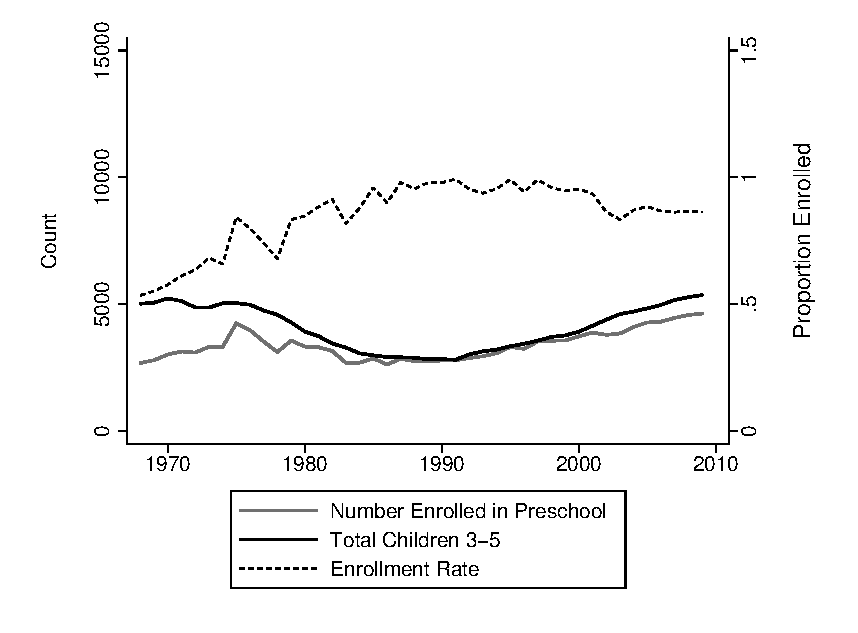
\includegraphics[width=\textwidth]{../../output/image/enrollment_vs_totalChildren_Reggio.eps}
%\end{subfigure}%
%~
%\begin{subfigure}[b]{0.55\textwidth}
%	\caption{Padova}\label{fig:enrollmentRatePadova}
%	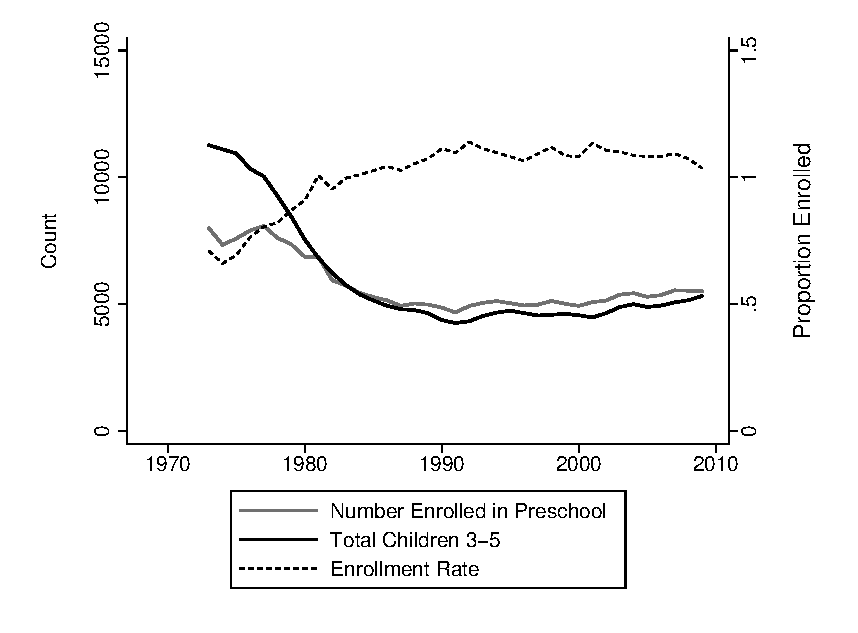
\includegraphics[width=\textwidth]{../../output/image/enrollment_vs_totalChildren_Padova.eps}
%\end{subfigure}%
%\end{center}
%\raggedright \footnotesize Note: These graphs show the trend in enrollment rates in Reggio Emilia and Padova over time. The series measuring preschool enrollment is not restricted to the 3-5 age group, and thus, is allowed to be greater than the series for total children 3-5. The enrollment proportion is occasionally greater than 1 in Padova due to this reason. See Appendix~\ref{app:characteristics-cities} for information on the sources used to construct these graphs.
%\end{figure}
%
%This information provides evidence of the extent to which alternative preschools were available and utilized. Comparing a individuals who attended one preschool program to those who attended another one can result in few outcomes, especially if the alternative preschools offer quality education. In fact, when we compare adults who attended some types of preschool in Padova with adults who did not attend any preschool in Padova, the estimation results show that the preschool attendance in Padova has significantly positive effects on IQ, university graduation, obesity, and voting behaviors for the age-30 cohort (See Appendix \ref{subsection:padova-estimation} for more specific results). This suggests that Padova had quality preschool education system from the 1970s. 

\clearpage

\bibliography{heckman}
\bibliographystyle{chicago}


\end{document}
